% Author: Alfredo Sánchez Alberca (asalber@gmail.com)
\section{Frequency distributions: Tabulation and charts}

\mode<presentation>{
%---------------------------------------------------------------------slide----
\begin{frame}
\frametitle{Frequency distribution: Tabulation and charts}
\tableofcontents[sectionstyle=show/hide,hideothersubsections]
\end{frame}
}


%---------------------------------------------------------------------slide----
\begin{frame} 
\frametitle{Descriptive Statistics}
Descriptive Statistics is the part of Statistics in charge of representing, analysing and summarizing the information
contained in the sample.

After the sampling process, is the next step in every statistical study and usually consists of:
\begin{enumerate}
\item Classify, group and sort the data of the sample.
\item Tabulate and plot data according to their frequencies.
\item Calculate numerical measures that summarize the information contained in the sample (\emph{sample statistics}).
\end{enumerate} 

It has no inferential power $\Rightarrow$ \alert{\emph{Do not generalize to the population!}} 
\end{frame}


\subsection{Frequency distribution}
%---------------------------------------------------------------------slide----
\begin{frame}
\frametitle{Sample classification}
The study of a statistical variable starts measuring the variable in the individuals of the sample and classifying the
values.

There are two ways of classifying data:
\begin{description}
\item[Non-grouping] Sort values from lowest to highest value (if there is an order).
Used with qualitative variables and discrete variables with few distinct values.
\item[Grouping] Group values in intervals (classes) and sort them from lowest to highest intervals. 
Used with continuous variables and discrete variables with many distinct values. 
\end{description}
\end{frame}


%---------------------------------------------------------------------slide----
\begin{frame}
\frametitle{Sample classification}
$X=$Height
\begin{center}
\tikzsetnextfilename{descriptive/sample_classification}
\scalebox{0.6}{% Autor: Alfredo Sánchez Alberca (email:asalber@ceu.es)
% Charts that shows the purpose of Statistics
\begin{tikzpicture}[every label/.style={text=color1}]
\node (sample) at (0,8) {\includegraphics[height=4cm]{img/descriptive/sample.png}}; 
\pause
\node (ordered-sample) at (0,0) {\includegraphics[height=4cm]{img/descriptive/ordered_sample.png}};
\node at (0,4) [fill=color2,single arrow,shape border rotate=270,minimum height=3cm,text=white, minimum width=4cm]{\huge
\ Classify\ \phantom{}};
\end{tikzpicture} }
\end{center}
\end{frame}


%---------------------------------------------------------------------slide----
\begin{frame}
\frametitle{Frequency count}
$X=$Height
\begin{center}
\tikzsetnextfilename{descriptive/frequency_count}
\scalebox{0.6}{% Autor: Alfredo Sánchez Alberca (email:asalber@ceu.es)
% Charts that shows the purpose of Statistics
\begin{tikzpicture}[every label/.style={text=color1}]
\node at (0,8) {\includegraphics[height=4cm]{img/descriptive/ordered_sample.png}}; 
\pause
\node at (0,0) {\includegraphics[height=4cm]{img/descriptive/sample_frequencies.png}};
\node at (0,4) [fill=color1,single arrow,shape border rotate=270,minimum height=3cm,text=white, minimum
width=4cm, align=center]{\huge Frequency\\ \huge count};
\end{tikzpicture} }
\end{center}
\end{frame}


%---------------------------------------------------------------------slide----
\begin{frame}
\frametitle{Sample frequencies}
\begin{definition}[Sample frequencies]
Given a sample of $n$ values of a variable $X$, for every value $x_i$ of the variable
is defined 
\begin{itemize}
\item \highlight{Absolute frequency $n_i$}: Is the number of times that value $x_i$ appears in the sample.
\item \highlight{Relative frequency $f_i$}: Is the proportion of times that value $x_i$ appears in the sample.
\[
f_i = \frac{n_i}{n}
\]
\item \highlight{Cumulative absolute frequency $N_i$}: Is the number of values in the sample less than or equal to
$x_i$.
\[
N_i = n_1 + \cdots + n_i
\]
\item \highlight{Cumulative relative frequency $F_i$}: Is the proportion of values in the sample less than or equal to
$x_i$.
\[
F_i = \frac{N_i}{n}
\]
\end{itemize}
\end{definition}
\end{frame}


%---------------------------------------------------------------------slide----
\begin{frame}
\frametitle{Frequency table}
The set of values of a variable with their respective frequencies is called \highlight{\textbf{frequency distribution}}
of the variable in the sample, and it is usually represented as a \highlight{\textbf{frequency table}}.
\begin{center}
\begin{tabular}{|>{\centering}p{1.8cm}|>{\centering}p{1.8cm}|>{\centering}p{1.8cm}|>{\centering}p{1.8cm}|p{1.8cm}<{\centering}|}
\hline
\highlight{$X$ values} & \highlight{Absolute frequency} & \highlight{Relative frequency} & \highlight{Cumulative
absolute frequency} & \highlight{Cumulative relative frequency} \\
\hline
$x_1$ & $n_1$ & $f_1$ & $N_1$ & $F_1$\\
$\vdots$ & $\vdots$ & $\vdots$ & $\vdots$ & $\vdots$\\
$x_i$ & $n_i$ & $f_i$ & $N_i$ & $F_i$\\
$\vdots$ & $\vdots$ & $\vdots$ & $\vdots$ & $\vdots$\\
$x_k$ & $n_k$ & $f_k$ & $N_k$ & $F_k$\\
\hline
\end{tabular}
\end{center}
\end{frame}


%---------------------------------------------------------------------slide----
\begin{frame}
\frametitle{Frequency table}
\framesubtitle{Example of quantitative variable and non-grouped data}
The number of children in 25 families are:
\begin{center}
1, 2, 4, 2, 2, 2, 3, 2, 1, 1, 0, 2, 2, \\
 0, 2, 2, 1, 2, 2, 3, 1, 2, 2, 1, 2
\end{center}
The frequency table for the number of children in this sample is 
\[
\setlength\arraycolsep{3mm}
\setlength\arrayrulewidth{0.5pt}
\begin{array}{rrrrr}
\hline
x_i & n_i & f_i & N_i & F_i\\
\hline
0 & 2 & 0.08 & 2 & 0.08\\
1 & 6 & 0.24 & 8 & 0.32\\
2 & 14 & 0.56 & 22 & 0.88\\
3 & 2  & 0.08 & 24 & 0.96\\
4 & 1 & 0.04 & 25 & 1 \\
\hline
\sum & 25 & 1 \\
\hline
\end{array}
\]
\end{frame}


%---------------------------------------------------------------------slide----
\begin{frame}
\frametitle{Frequency table}
\framesubtitle{Example of quantitative variable and grouped data}
The heights (in cm) of 30 students are:
\begin{center}
179, 173, 181, 170, 158, 174, 172, 166, 194, 185,\\
162, 187, 198, 177, 178, 165, 154, 188, 166, 171,\\
175, 182, 167, 169, 172, 186, 172, 176, 168, 187.
\end{center}
The frequency table for the height in this sample is
\[
\setlength\arraycolsep{3mm}
\setlength\arrayrulewidth{0.5pt}
\begin{array}{rrrrr}
\hline
\multicolumn{1}{c}{x_i} & \multicolumn{1}{c}{n_i} & \multicolumn{1}{c}{f_i} & \multicolumn{1}{c}{N_i} & \multicolumn{1}{c}{F_i}\\
\hline
(150,160] & 2 & 0.07 & 2 & 0.07\\
(160,170] & 8 & 0.27 & 10 & 0.34\\
(170,180] & 11 & 0.36 & 21 & 0.70\\
(180,190] & 7  & 0.23 & 28 & 0.93\\
(190,200] & 2 & 0.07 & 30 & 1 \\
\hline
\sum & 30 & 1 \\
\hline
\end{array}
\]
\end{frame}


%---------------------------------------------------------------------slide----
\begin{frame}
\frametitle{Classes construction}
Intervals are known as \highlight{\textbf{classes}} and the center of intervals as \highlight{\textbf{class marks}}.

When grouping data into intervals, the following rules must be taken into account: 
\begin{itemize}
\item The number of intervals should not be too big nor too small. 
A usual rule of thumb is to take a number of intervals approximately $\sqrt{n}$ or $\log_2(n)$.
\item The intervals must not overlap and must cover the entire range of values.
It doesn't matter if intervals are left-open and right-closed or vice versa. 
\item The minimum value must fall in the first interval and the maximum value in the last.
\end{itemize}
\end{frame}


%---------------------------------------------------------------------slide----
\begin{frame}
\frametitle{Frequency table}
\framesubtitle{Example with qualitative variable}
The blood type of 30 people are:
\begin{center}
A, B, B, A, AB, 0, 0, A, B, B, A, A, A, A, AB,\\
A, A, A, B, 0, B, B, B, A, A, A, 0, A, AB, 0.
\end{center}
The frequency table of the blood type is 
\[
\setlength\arraycolsep{3mm}
\setlength\arrayrulewidth{0.5pt}
\begin{array}{crr}
\hline
\multicolumn{1}{c}{x_i} & \multicolumn{1}{c}{n_i} & \multicolumn{1}{c}{f_i} \\
\hline
\mbox{0} & 5 & 0.16 \\
\mbox{A} & 14 & 0.47 \\
\mbox{B} & 8 & 0.27 \\
\mbox{AB} & 3 & 0.10 \\
\hline
\sum & 30 & 1 \\
\hline
\end{array}
\]
\begin{center}
\emph{Why there are not cumulative frequencies?}
\end{center} 
\end{frame}


\subsection{Frequency distribution graphs}

%---------------------------------------------------------------------slide----
\begin{frame}
\frametitle{Frequency distribution graphs}
Usually the frequency distribution is also displayed graphically.
 
Depending on the type of variable and if data has been grouped or not, there are different types of charts:
\begin{itemize}
\item Bar chart
\item Histogram
\item Line chart
\item Pie chart
\end{itemize}
\end{frame} 


%---------------------------------------------------------------------slide----
\begin{frame}
\frametitle{Bar chart}
A \highlight{bar chart} consists in a set of bars, one for every value or category of the variable, plotted on a
coordinate system.

Usually the values or categories of the variable are represented on the $x$-axis, and the frequencies on the $y$-axis. 
For each value or category of the variable, a bar is draw to the height of its frequency.
The width of the bar is not important but bars should be clearly separated among them. 

Depending on the type of frequency represented in the $y$-axis we get different types of bar charts.
 
Sometimes a polygon, known as \highlight{\textbf{frequency polygon}}, is plotted joining the top of every bar with
straight lines.
\end{frame}



%---------------------------------------------------------------------slide----
\begin{frame}
\frametitle{Absolute frequency bar chart}
\framesubtitle{Non-grouped data}
\begin{center}
\tikzsetnextfilename{descriptive/abs_freq_bar_chart}
\scalebox{0.6}{\input{img/descriptive/abs_freq_bar_chart}} 
\end{center}
\end{frame}


%---------------------------------------------------------------------slide----
\begin{frame}
\frametitle{Absolute frequency line chart or polygon}
\framesubtitle{Non-grouped data}
\begin{center}
\tikzsetnextfilename{descriptive/abs_freq_bar_chart_polygon}
\scalebox{0.6}{% Created by tikzDevice version 0.8.1 on 2015-11-06 00:42:54
% !TEX encoding = UTF-8 Unicode
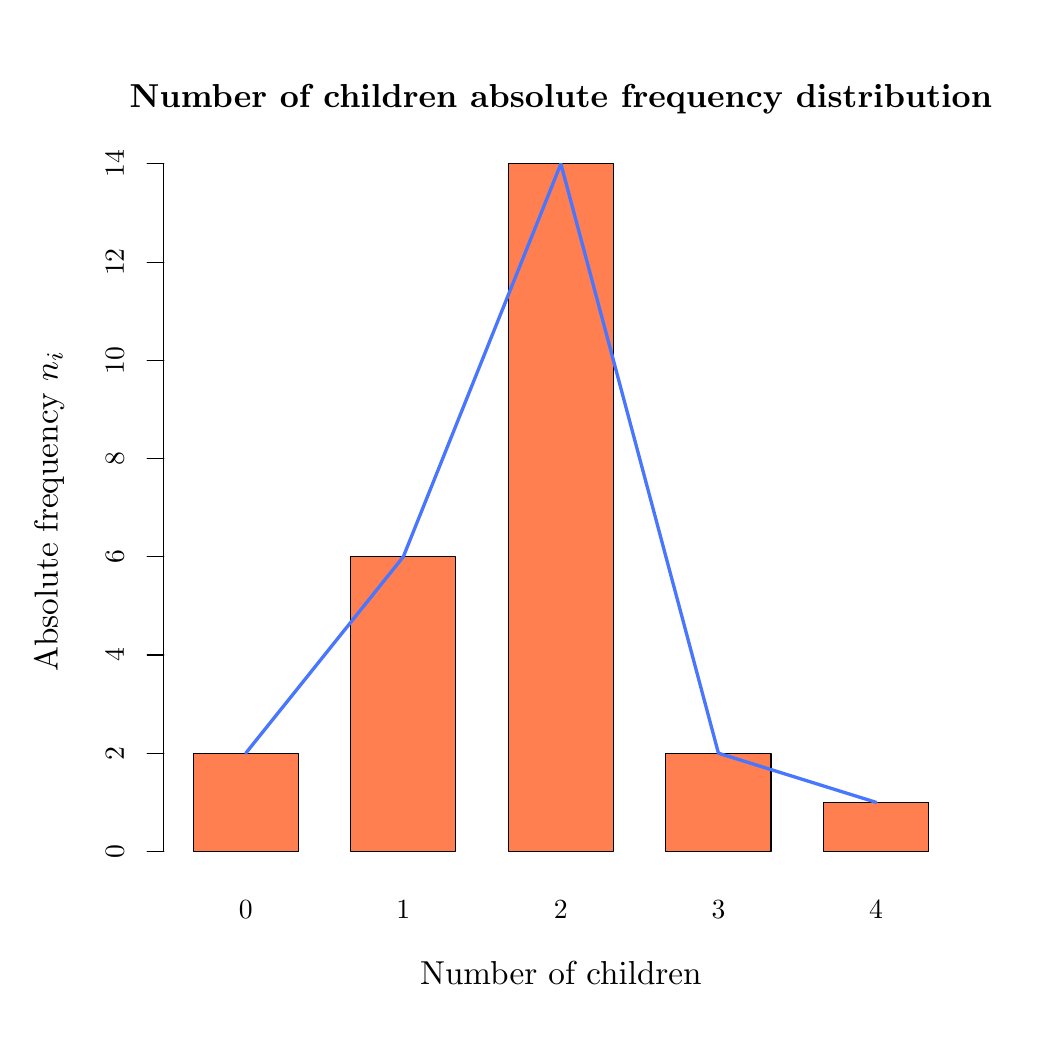
\begin{tikzpicture}[x=1pt,y=1pt]
\definecolor{fillColor}{RGB}{255,255,255}
\path[use as bounding box,fill=fillColor,fill opacity=0.00] (0,0) rectangle (361.35,361.35);
\begin{scope}
\path[clip] (  0.00,  0.00) rectangle (361.35,361.35);
\definecolor{drawColor}{RGB}{0,0,0}
\definecolor{fillColor}{RGB}{255,127,80}

\path[draw=drawColor,line width= 0.4pt,line join=round,line cap=round,fill=fillColor] ( 59.83, 63.68) rectangle ( 97.78, 99.18);

\path[draw=drawColor,line width= 0.4pt,line join=round,line cap=round,fill=fillColor] (116.76, 63.68) rectangle (154.72,170.17);

\path[draw=drawColor,line width= 0.4pt,line join=round,line cap=round,fill=fillColor] (173.70, 63.68) rectangle (211.65,312.15);

\path[draw=drawColor,line width= 0.4pt,line join=round,line cap=round,fill=fillColor] (230.63, 63.68) rectangle (268.59, 99.18);

\path[draw=drawColor,line width= 0.4pt,line join=round,line cap=round,fill=fillColor] (287.57, 63.68) rectangle (325.52, 81.43);
\end{scope}
\begin{scope}
\path[clip] (  0.00,  0.00) rectangle (361.35,361.35);
\definecolor{drawColor}{RGB}{0,0,0}

\node[text=drawColor,anchor=base,inner sep=0pt, outer sep=0pt, scale=  1.00] at ( 78.81, 39.60) {0};

\node[text=drawColor,anchor=base,inner sep=0pt, outer sep=0pt, scale=  1.00] at (135.74, 39.60) {1};

\node[text=drawColor,anchor=base,inner sep=0pt, outer sep=0pt, scale=  1.00] at (192.67, 39.60) {2};

\node[text=drawColor,anchor=base,inner sep=0pt, outer sep=0pt, scale=  1.00] at (249.61, 39.60) {3};

\node[text=drawColor,anchor=base,inner sep=0pt, outer sep=0pt, scale=  1.00] at (306.54, 39.60) {4};
\end{scope}
\begin{scope}
\path[clip] (  0.00,  0.00) rectangle (361.35,361.35);
\definecolor{drawColor}{RGB}{0,0,0}

\node[text=drawColor,anchor=base,inner sep=0pt, outer sep=0pt, scale=  1.20] at (192.68,332.61) {\bfseries Number of children absolute frequency distribution};

\node[text=drawColor,anchor=base,inner sep=0pt, outer sep=0pt, scale=  1.20] at (192.68, 15.60) {Number of children};

\node[text=drawColor,rotate= 90.00,anchor=base,inner sep=0pt, outer sep=0pt, scale=  1.20] at ( 10.80,186.67) {Absolute frequency $n_i$};
\end{scope}
\begin{scope}
\path[clip] (  0.00,  0.00) rectangle (361.35,361.35);
\definecolor{drawColor}{RGB}{0,0,0}

\path[draw=drawColor,line width= 0.4pt,line join=round,line cap=round] ( 49.20, 63.68) -- ( 49.20,312.15);

\path[draw=drawColor,line width= 0.4pt,line join=round,line cap=round] ( 49.20, 63.68) -- ( 43.20, 63.68);

\path[draw=drawColor,line width= 0.4pt,line join=round,line cap=round] ( 49.20, 99.18) -- ( 43.20, 99.18);

\path[draw=drawColor,line width= 0.4pt,line join=round,line cap=round] ( 49.20,134.67) -- ( 43.20,134.67);

\path[draw=drawColor,line width= 0.4pt,line join=round,line cap=round] ( 49.20,170.17) -- ( 43.20,170.17);

\path[draw=drawColor,line width= 0.4pt,line join=round,line cap=round] ( 49.20,205.66) -- ( 43.20,205.66);

\path[draw=drawColor,line width= 0.4pt,line join=round,line cap=round] ( 49.20,241.16) -- ( 43.20,241.16);

\path[draw=drawColor,line width= 0.4pt,line join=round,line cap=round] ( 49.20,276.65) -- ( 43.20,276.65);

\path[draw=drawColor,line width= 0.4pt,line join=round,line cap=round] ( 49.20,312.15) -- ( 43.20,312.15);

\node[text=drawColor,rotate= 90.00,anchor=base,inner sep=0pt, outer sep=0pt, scale=  1.00] at ( 34.80, 63.68) {0};

\node[text=drawColor,rotate= 90.00,anchor=base,inner sep=0pt, outer sep=0pt, scale=  1.00] at ( 34.80, 99.18) {2};

\node[text=drawColor,rotate= 90.00,anchor=base,inner sep=0pt, outer sep=0pt, scale=  1.00] at ( 34.80,134.67) {4};

\node[text=drawColor,rotate= 90.00,anchor=base,inner sep=0pt, outer sep=0pt, scale=  1.00] at ( 34.80,170.17) {6};

\node[text=drawColor,rotate= 90.00,anchor=base,inner sep=0pt, outer sep=0pt, scale=  1.00] at ( 34.80,205.66) {8};

\node[text=drawColor,rotate= 90.00,anchor=base,inner sep=0pt, outer sep=0pt, scale=  1.00] at ( 34.80,241.16) {10};

\node[text=drawColor,rotate= 90.00,anchor=base,inner sep=0pt, outer sep=0pt, scale=  1.00] at ( 34.80,276.65) {12};

\node[text=drawColor,rotate= 90.00,anchor=base,inner sep=0pt, outer sep=0pt, scale=  1.00] at ( 34.80,312.15) {14};
\end{scope}
\begin{scope}
\path[clip] ( 49.20, 61.20) rectangle (336.15,312.15);
\definecolor{drawColor}{RGB}{72,118,255}

\path[draw=drawColor,line width= 1.2pt,line join=round,line cap=round] ( 78.81, 99.18) --
	(135.74,170.17) --
	(192.67,312.15) --
	(249.61, 99.18) --
	(306.54, 81.43);
\end{scope}
\end{tikzpicture}
} 
\end{center}
\end{frame}


%---------------------------------------------------------------------slide----
\begin{frame}
\frametitle{Cumulative absolute frequency bar chart}
\framesubtitle{Non-grouped data}
\begin{center}
\tikzsetnextfilename{descriptive/cum_abs_freq_bar_chart}
\scalebox{0.6}{\input{img/descriptive/cum_abs_freq_bar_chart}} 
\end{center}
\end{frame}


%---------------------------------------------------------------------slide----
\begin{frame}
\frametitle{Cumulative absolute frequency line chart or polygon}
\framesubtitle{Non-grouped data}
\begin{center}
\tikzsetnextfilename{descriptive/cum_abs_freq_bar_chart_polygon}
\scalebox{0.6}{% Created by tikzDevice version 0.8.1 on 2015-11-09 17:45:22
% !TEX encoding = UTF-8 Unicode
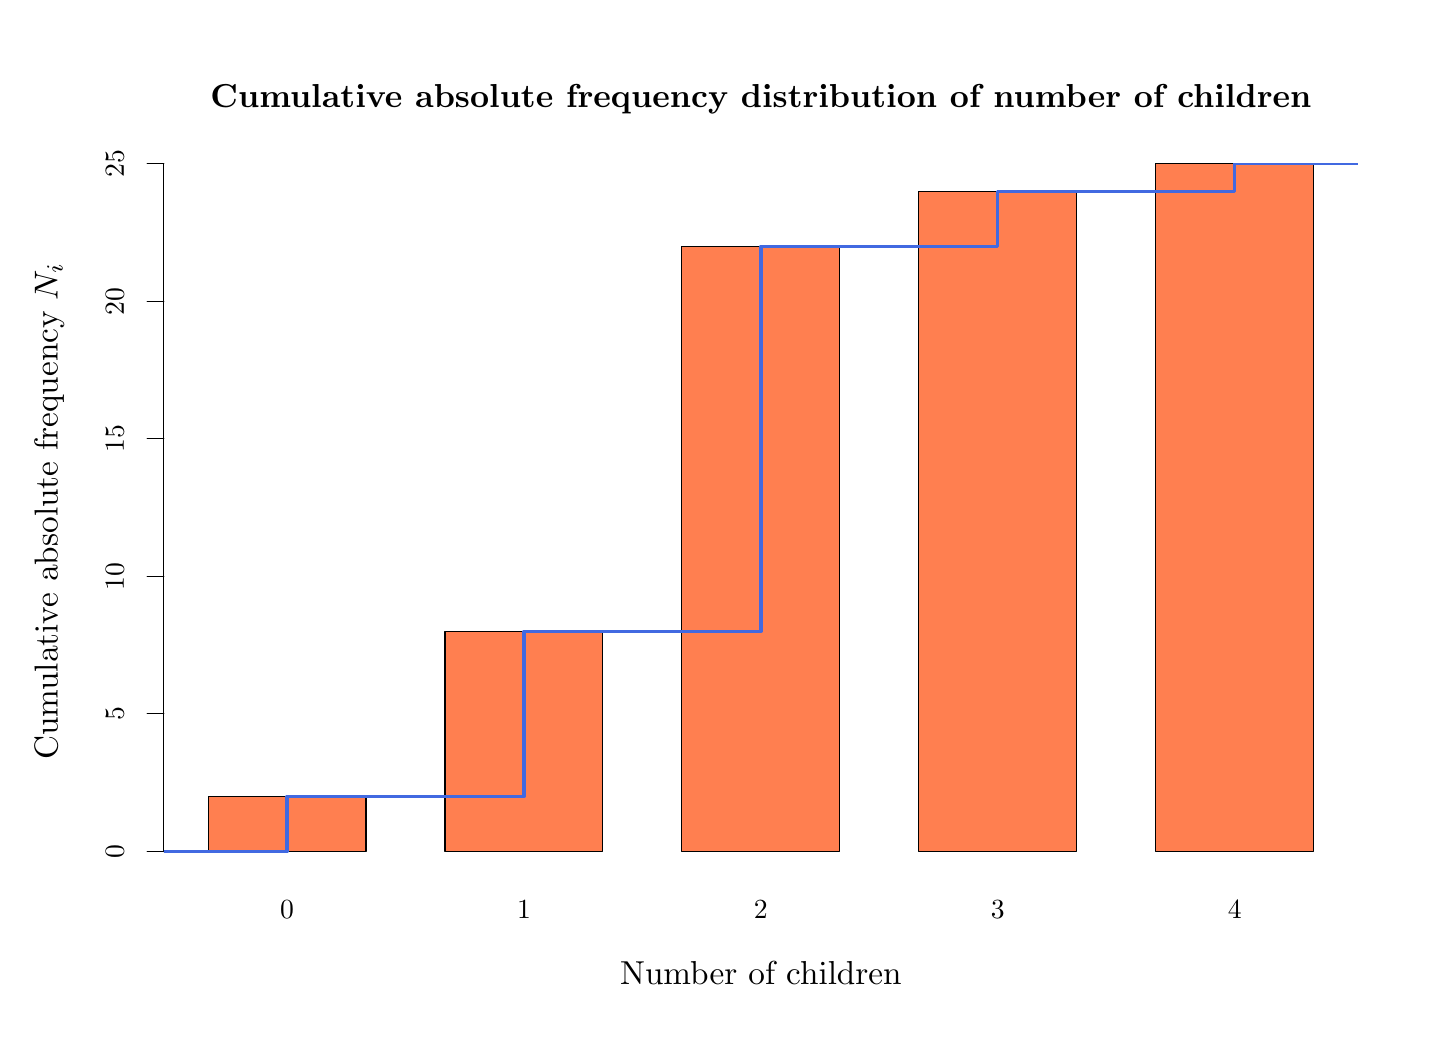
\begin{tikzpicture}[x=1pt,y=1pt]
\definecolor{fillColor}{RGB}{255,255,255}
\path[use as bounding box,fill=fillColor,fill opacity=0.00] (0,0) rectangle (505.89,361.35);
\begin{scope}
\path[clip] (  0.00,  0.00) rectangle (505.89,361.35);
\definecolor{drawColor}{RGB}{0,0,0}
\definecolor{fillColor}{RGB}{255,127,80}

\path[draw=drawColor,line width= 0.4pt,line join=round,line cap=round,fill=fillColor] ( 65.18, 63.68) rectangle (122.26, 83.56);

\path[draw=drawColor,line width= 0.4pt,line join=round,line cap=round,fill=fillColor] (150.79, 63.68) rectangle (207.87,143.19);

\path[draw=drawColor,line width= 0.4pt,line join=round,line cap=round,fill=fillColor] (236.41, 63.68) rectangle (293.48,282.33);

\path[draw=drawColor,line width= 0.4pt,line join=round,line cap=round,fill=fillColor] (322.02, 63.68) rectangle (379.10,302.21);

\path[draw=drawColor,line width= 0.4pt,line join=round,line cap=round,fill=fillColor] (407.63, 63.68) rectangle (464.71,312.15);
\end{scope}
\begin{scope}
\path[clip] (  0.00,  0.00) rectangle (505.89,361.35);
\definecolor{drawColor}{RGB}{0,0,0}

\node[text=drawColor,anchor=base,inner sep=0pt, outer sep=0pt, scale=  1.00] at ( 93.72, 39.60) {0};

\node[text=drawColor,anchor=base,inner sep=0pt, outer sep=0pt, scale=  1.00] at (179.33, 39.60) {1};

\node[text=drawColor,anchor=base,inner sep=0pt, outer sep=0pt, scale=  1.00] at (264.94, 39.60) {2};

\node[text=drawColor,anchor=base,inner sep=0pt, outer sep=0pt, scale=  1.00] at (350.56, 39.60) {3};

\node[text=drawColor,anchor=base,inner sep=0pt, outer sep=0pt, scale=  1.00] at (436.17, 39.60) {4};
\end{scope}
\begin{scope}
\path[clip] (  0.00,  0.00) rectangle (505.89,361.35);
\definecolor{drawColor}{RGB}{0,0,0}

\node[text=drawColor,anchor=base,inner sep=0pt, outer sep=0pt, scale=  1.20] at (264.94,332.61) {\bfseries Cumulative absolute frequency distribution of number of children};

\node[text=drawColor,anchor=base,inner sep=0pt, outer sep=0pt, scale=  1.20] at (264.94, 15.60) {Number of children};

\node[text=drawColor,rotate= 90.00,anchor=base,inner sep=0pt, outer sep=0pt, scale=  1.20] at ( 10.80,186.67) {Cumulative absolute frequency $N_i$};
\end{scope}
\begin{scope}
\path[clip] (  0.00,  0.00) rectangle (505.89,361.35);
\definecolor{drawColor}{RGB}{0,0,0}

\path[draw=drawColor,line width= 0.4pt,line join=round,line cap=round] ( 49.20, 63.68) -- ( 49.20,312.15);

\path[draw=drawColor,line width= 0.4pt,line join=round,line cap=round] ( 49.20, 63.68) -- ( 43.20, 63.68);

\path[draw=drawColor,line width= 0.4pt,line join=round,line cap=round] ( 49.20,113.38) -- ( 43.20,113.38);

\path[draw=drawColor,line width= 0.4pt,line join=round,line cap=round] ( 49.20,163.07) -- ( 43.20,163.07);

\path[draw=drawColor,line width= 0.4pt,line join=round,line cap=round] ( 49.20,212.76) -- ( 43.20,212.76);

\path[draw=drawColor,line width= 0.4pt,line join=round,line cap=round] ( 49.20,262.46) -- ( 43.20,262.46);

\path[draw=drawColor,line width= 0.4pt,line join=round,line cap=round] ( 49.20,312.15) -- ( 43.20,312.15);

\node[text=drawColor,rotate= 90.00,anchor=base,inner sep=0pt, outer sep=0pt, scale=  1.00] at ( 34.80, 63.68) {0};

\node[text=drawColor,rotate= 90.00,anchor=base,inner sep=0pt, outer sep=0pt, scale=  1.00] at ( 34.80,113.38) {5};

\node[text=drawColor,rotate= 90.00,anchor=base,inner sep=0pt, outer sep=0pt, scale=  1.00] at ( 34.80,163.07) {10};

\node[text=drawColor,rotate= 90.00,anchor=base,inner sep=0pt, outer sep=0pt, scale=  1.00] at ( 34.80,212.76) {15};

\node[text=drawColor,rotate= 90.00,anchor=base,inner sep=0pt, outer sep=0pt, scale=  1.00] at ( 34.80,262.46) {20};

\node[text=drawColor,rotate= 90.00,anchor=base,inner sep=0pt, outer sep=0pt, scale=  1.00] at ( 34.80,312.15) {25};
\end{scope}
\begin{scope}
\path[clip] ( 49.20, 61.20) rectangle (480.69,312.15);
\definecolor{drawColor}{RGB}{65,105,225}

\path[draw=drawColor,line width= 1.2pt,line join=round,line cap=round] ( 36.64, 63.68) --
	( 93.72, 63.68) --
	( 93.72, 83.56) --
	(179.33, 83.56) --
	(179.33,143.19) --
	(264.94,143.19) --
	(264.94,282.33) --
	(350.56,282.33) --
	(350.56,302.21) --
	(436.17,302.21) --
	(436.17,312.15) --
	(505.89,312.15);
\end{scope}
\end{tikzpicture}
} 
\end{center} 
\end{frame}


%---------------------------------------------------------------------slide----
\begin{frame}
\frametitle{Histogram}
A \highlight{histogram} is similar to a bar chart but for grouped data.  

Usually the classes or grouping intervals are represented on the $x$-axis, and the frequencies on the $y$-axis. 
For each class, a bar is draw to the height of its frequency.
Contrary to bar charts, the width of bars coincides with the width of classes, and there are no space between two
consecutive bars.

Depending on the type of frequency represented in the $y$-axis we get different types of histograms.
 
Sometimes a polygon, known as \highlight{\textbf{frequency polygon}}, is plotted joining the top of every bar.
\end{frame}


%---------------------------------------------------------------------slide----
\begin{frame}
\frametitle{Absolute frequency histogram}
\framesubtitle{Grouped data}
\begin{center}
\tikzsetnextfilename{descriptive/abs_freq_histogram}
\scalebox{0.6}{% Created by tikzDevice version 0.8.1 on 2015-11-09 19:19:11
% !TEX encoding = UTF-8 Unicode
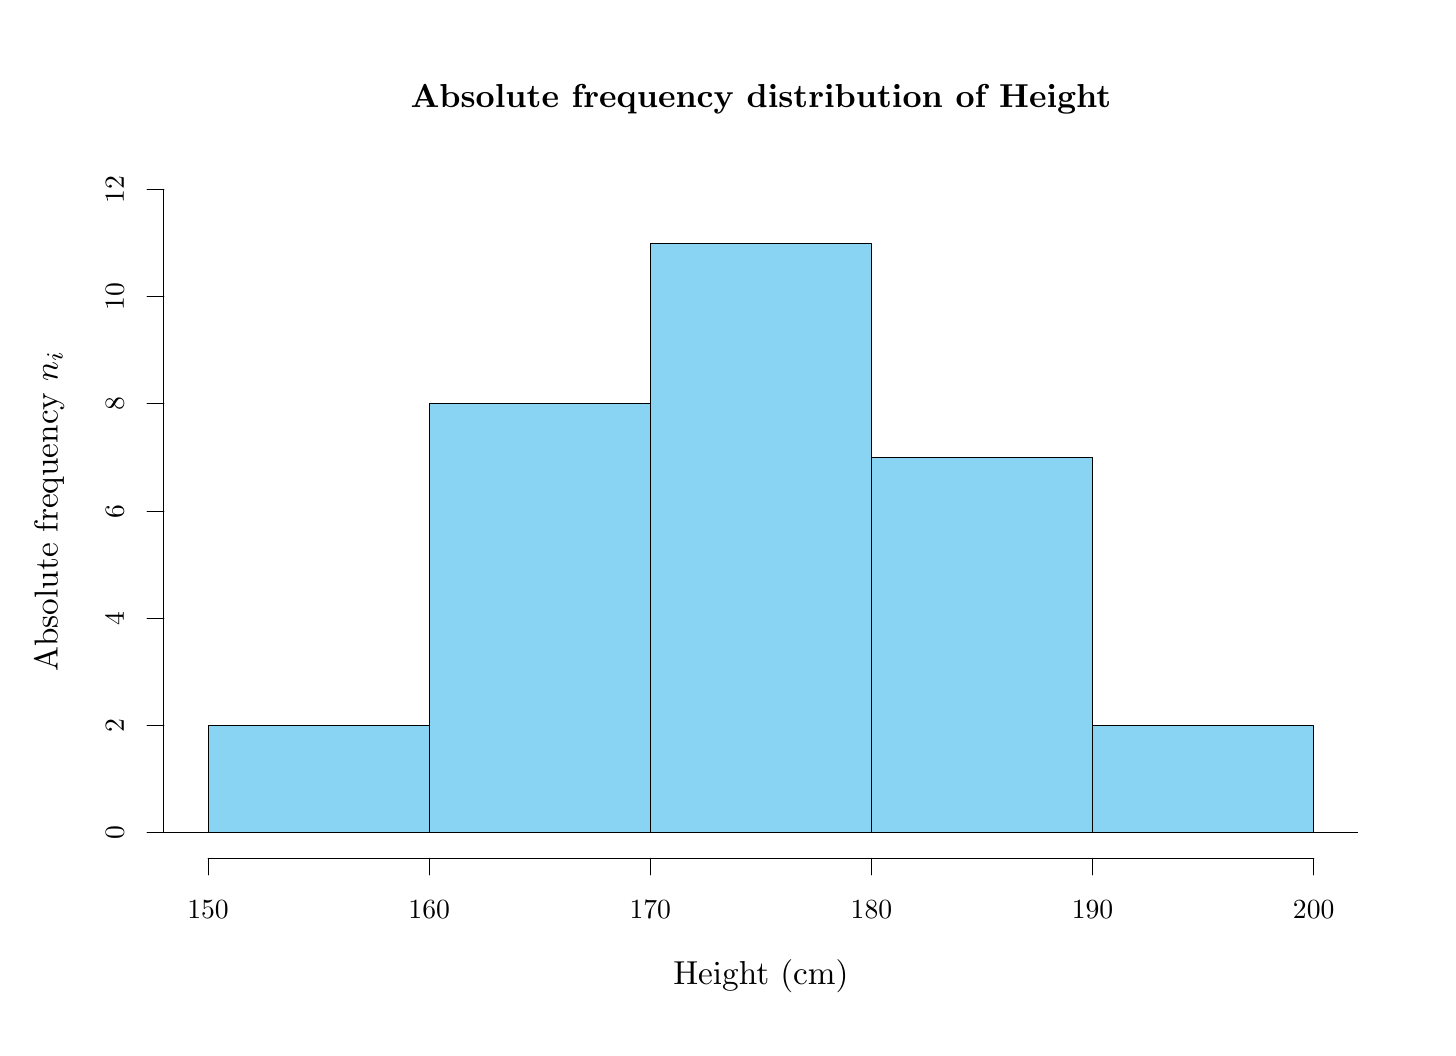
\begin{tikzpicture}[x=1pt,y=1pt]
\definecolor{fillColor}{RGB}{255,255,255}
\path[use as bounding box,fill=fillColor,fill opacity=0.00] (0,0) rectangle (505.89,361.35);
\begin{scope}
\path[clip] (  0.00,  0.00) rectangle (505.89,361.35);
\definecolor{drawColor}{RGB}{0,0,0}

\node[text=drawColor,anchor=base,inner sep=0pt, outer sep=0pt, scale=  1.20] at (264.95,332.61) {\bfseries Absolute frequency distribution of Height};

\node[text=drawColor,anchor=base,inner sep=0pt, outer sep=0pt, scale=  1.20] at (264.95, 15.60) {Height (cm)};

\node[text=drawColor,rotate= 90.00,anchor=base,inner sep=0pt, outer sep=0pt, scale=  1.20] at ( 10.80,186.67) {Absolute frequency $n_i$};
\end{scope}
\begin{scope}
\path[clip] (  0.00,  0.00) rectangle (505.89,361.35);
\definecolor{drawColor}{RGB}{0,0,0}

\path[draw=drawColor,line width= 0.4pt,line join=round,line cap=round] ( 65.18, 61.20) -- (464.71, 61.20);

\path[draw=drawColor,line width= 0.4pt,line join=round,line cap=round] ( 65.18, 61.20) -- ( 65.18, 55.20);

\path[draw=drawColor,line width= 0.4pt,line join=round,line cap=round] (145.09, 61.20) -- (145.09, 55.20);

\path[draw=drawColor,line width= 0.4pt,line join=round,line cap=round] (224.99, 61.20) -- (224.99, 55.20);

\path[draw=drawColor,line width= 0.4pt,line join=round,line cap=round] (304.90, 61.20) -- (304.90, 55.20);

\path[draw=drawColor,line width= 0.4pt,line join=round,line cap=round] (384.80, 61.20) -- (384.80, 55.20);

\path[draw=drawColor,line width= 0.4pt,line join=round,line cap=round] (464.71, 61.20) -- (464.71, 55.20);

\node[text=drawColor,anchor=base,inner sep=0pt, outer sep=0pt, scale=  1.00] at ( 65.18, 39.60) {150};

\node[text=drawColor,anchor=base,inner sep=0pt, outer sep=0pt, scale=  1.00] at (145.09, 39.60) {160};

\node[text=drawColor,anchor=base,inner sep=0pt, outer sep=0pt, scale=  1.00] at (224.99, 39.60) {170};

\node[text=drawColor,anchor=base,inner sep=0pt, outer sep=0pt, scale=  1.00] at (304.90, 39.60) {180};

\node[text=drawColor,anchor=base,inner sep=0pt, outer sep=0pt, scale=  1.00] at (384.80, 39.60) {190};

\node[text=drawColor,anchor=base,inner sep=0pt, outer sep=0pt, scale=  1.00] at (464.71, 39.60) {200};

\path[draw=drawColor,line width= 0.4pt,line join=round,line cap=round] ( 49.20, 70.49) -- ( 49.20,302.86);

\path[draw=drawColor,line width= 0.4pt,line join=round,line cap=round] ( 49.20, 70.49) -- ( 43.20, 70.49);

\path[draw=drawColor,line width= 0.4pt,line join=round,line cap=round] ( 49.20,109.22) -- ( 43.20,109.22);

\path[draw=drawColor,line width= 0.4pt,line join=round,line cap=round] ( 49.20,147.95) -- ( 43.20,147.95);

\path[draw=drawColor,line width= 0.4pt,line join=round,line cap=round] ( 49.20,186.67) -- ( 43.20,186.67);

\path[draw=drawColor,line width= 0.4pt,line join=round,line cap=round] ( 49.20,225.40) -- ( 43.20,225.40);

\path[draw=drawColor,line width= 0.4pt,line join=round,line cap=round] ( 49.20,264.13) -- ( 43.20,264.13);

\path[draw=drawColor,line width= 0.4pt,line join=round,line cap=round] ( 49.20,302.86) -- ( 43.20,302.86);

\node[text=drawColor,rotate= 90.00,anchor=base,inner sep=0pt, outer sep=0pt, scale=  1.00] at ( 34.80, 70.49) {0};

\node[text=drawColor,rotate= 90.00,anchor=base,inner sep=0pt, outer sep=0pt, scale=  1.00] at ( 34.80,109.22) {2};

\node[text=drawColor,rotate= 90.00,anchor=base,inner sep=0pt, outer sep=0pt, scale=  1.00] at ( 34.80,147.95) {4};

\node[text=drawColor,rotate= 90.00,anchor=base,inner sep=0pt, outer sep=0pt, scale=  1.00] at ( 34.80,186.67) {6};

\node[text=drawColor,rotate= 90.00,anchor=base,inner sep=0pt, outer sep=0pt, scale=  1.00] at ( 34.80,225.40) {8};

\node[text=drawColor,rotate= 90.00,anchor=base,inner sep=0pt, outer sep=0pt, scale=  1.00] at ( 34.80,264.13) {10};

\node[text=drawColor,rotate= 90.00,anchor=base,inner sep=0pt, outer sep=0pt, scale=  1.00] at ( 34.80,302.86) {12};
\end{scope}
\begin{scope}
\path[clip] ( 49.20, 61.20) rectangle (480.69,312.15);
\definecolor{drawColor}{RGB}{0,0,0}
\definecolor{fillColor}{RGB}{137,211,243}

\path[draw=drawColor,line width= 0.4pt,line join=round,line cap=round,fill=fillColor] ( 65.18, 70.49) rectangle (145.09,109.22);

\path[draw=drawColor,line width= 0.4pt,line join=round,line cap=round,fill=fillColor] (145.09, 70.49) rectangle (224.99,225.40);

\path[draw=drawColor,line width= 0.4pt,line join=round,line cap=round,fill=fillColor] (224.99, 70.49) rectangle (304.90,283.49);

\path[draw=drawColor,line width= 0.4pt,line join=round,line cap=round,fill=fillColor] (304.90, 70.49) rectangle (384.80,206.04);

\path[draw=drawColor,line width= 0.4pt,line join=round,line cap=round,fill=fillColor] (384.80, 70.49) rectangle (464.71,109.22);
\definecolor{drawColor}{RGB}{238,50,36}


\definecolor{drawColor}{RGB}{0,0,0}

\path[draw=drawColor,line width= 0.4pt,line join=round,line cap=round] ( 49.20, 70.49) -- (480.69, 70.49);
\end{scope}
\end{tikzpicture}
}
\end{center} 
\end{frame}


%---------------------------------------------------------------------slide----
\begin{frame}
\frametitle{Absolute frequency histogram}
\framesubtitle{Grouped data}
\begin{center}
\tikzsetnextfilename{descriptive/abs_freq_histogram_polygon}
\scalebox{0.6}{\input{img/descriptive/abs_freq_histogram_polygon}} 
\end{center} 
\end{frame}

\mode<presentation>{
%---------------------------------------------------------------------slide----
\begin{frame}
\frametitle{Cumulative absolute frequency histogram}
\framesubtitle{Grouped data}
\begin{center}
\tikzsetnextfilename{descriptive/cum_abs_freq_histogram}
\scalebox{0.6}{\input{img/descriptive/cum_abs_freq_histogram}}
\end{center} 
\end{frame}


%---------------------------------------------------------------------slide----
\begin{frame}
\frametitle{Cumulative absolute frequency line chart or ogive}
\framesubtitle{Grouped data}
\begin{center}
\tikzsetnextfilename{descriptive/cum_abs_freq_histogram_polygon}
\scalebox{0.6}{\input{img/descriptive/cum_abs_freq_histogram_polygon}} 
\end{center} 
\end{frame}
}

%---------------------------------------------------------------------slide----
\begin{frame}
\frametitle{Cumulative relative frequency histogram}
\framesubtitle{Grouped data}
\begin{center}
\tikzsetnextfilename{descriptive/cum_rel_freq_histogram}
\scalebox{0.6}{\input{img/descriptive/cum_rel_freq_histogram}}
\end{center} 
\end{frame}


\mode<article>{The cumulative frequency polygon (for absolute or relative frequencies) is known as \textbf{ogive}.}
%---------------------------------------------------------------------slide----
\begin{frame}
\frametitle{Cumulative relative frequency line chart or ogive}
\framesubtitle{Grouped data}
\begin{center}
\tikzsetnextfilename{descriptive/cum_rel_freq_histogram_polygon}
\scalebox{0.6}{\input{img/descriptive/cum_rel_freq_histogram_polygon}} 
\end{center} 
\end{frame}
\mode<article>{Observe that in the ogive we join the top right corner of bars with straight lines, instead of the top
center, cause we don't reach the accumulated frequency of the class until the end of the interval.}
 

%---------------------------------------------------------------------slide----
\begin{frame}
\frametitle{Pie chart}
A \highlight{pie chart} consists in a circle divided in slices, one for every value or category of the variable. 
Each slice is called \highlight{sector} and its angle or area is proportional to the frequency of the corresponding
value or category. 

Pie charts can represent absolute or relative frequencies, but not cumulative frequencies, and are used with nominal
qualitative variables.
For ordinal qualitative or quantitative variables is better to use bar charts or histograms, cause it's easier to
perceive differences in one dimension (length of bars) than in two dimensions (areas of sectors).
\end{frame}


%---------------------------------------------------------------------slide----
\begin{frame}
\frametitle{Pie chart}
\framesubtitle{Nominal variables}
\begin{center}
\tikzsetnextfilename{descriptive/rel_freq_pie_chart}
\scalebox{0.6}{% Created by tikzDevice version 0.8.1 on 2015-11-09 20:32:18
% !TEX encoding = UTF-8 Unicode
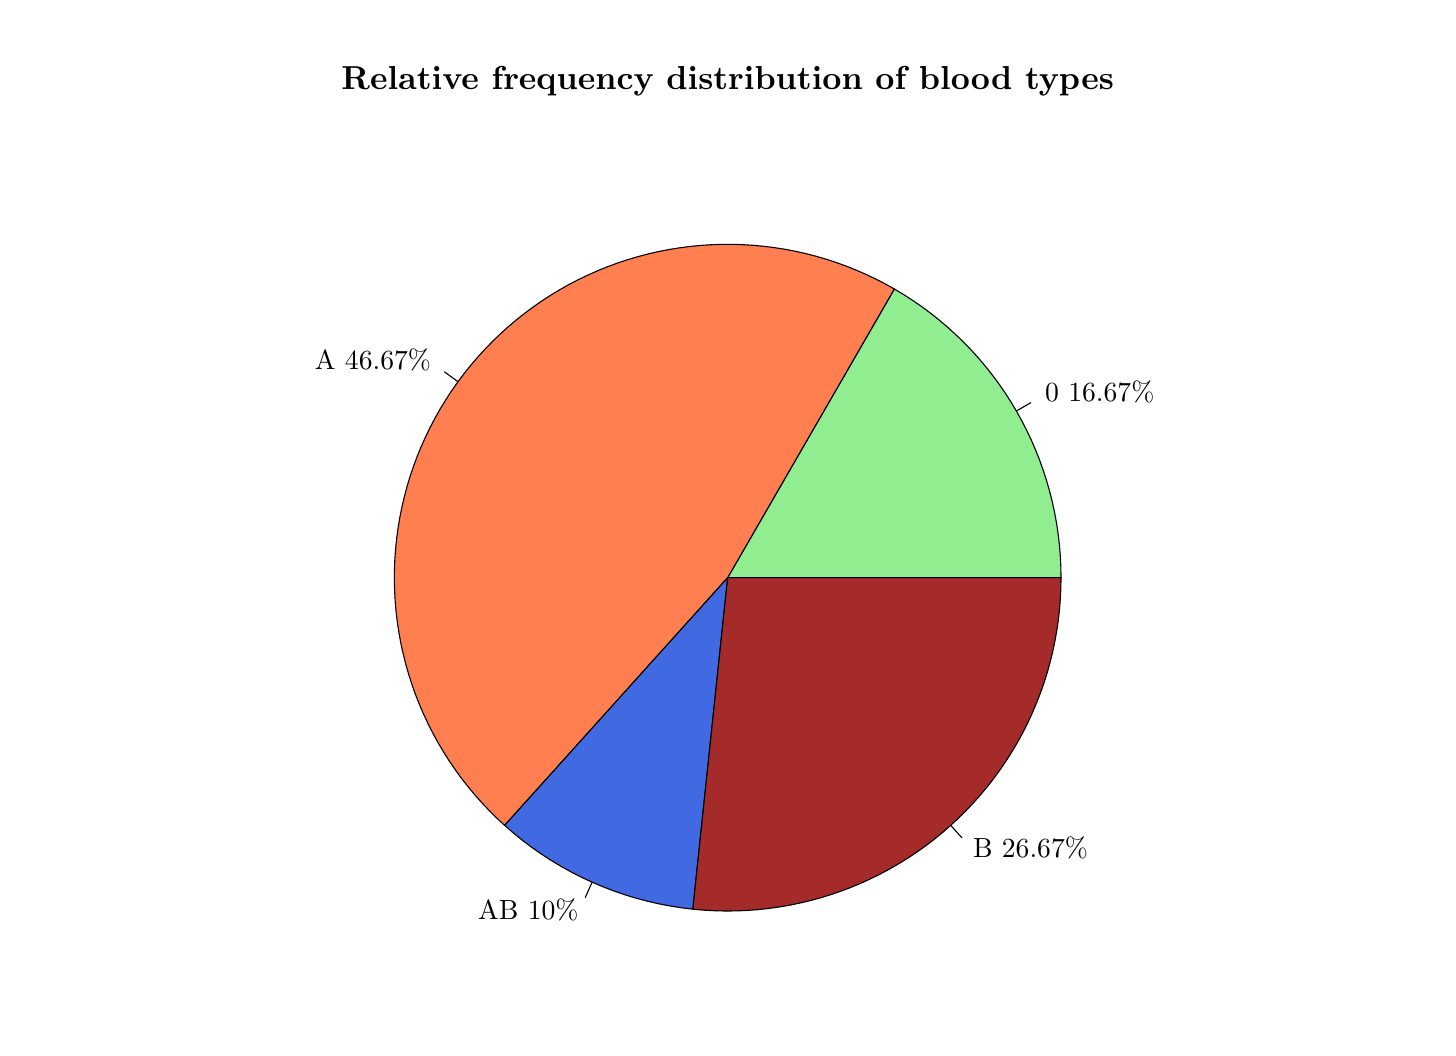
\begin{tikzpicture}[x=1pt,y=1pt]
\definecolor{fillColor}{RGB}{255,255,255}
\path[use as bounding box,fill=fillColor,fill opacity=0.00] (0,0) rectangle (505.89,361.35);
\begin{scope}
\path[clip] (  0.00,  0.00) rectangle (505.89,325.21);
\definecolor{drawColor}{RGB}{0,0,0}
\definecolor{fillColor}{RGB}{144,238,144}

\path[draw=drawColor,line width= 0.4pt,line join=round,line cap=round,fill=fillColor] (373.40,162.61) --
	(373.33,166.55) --
	(373.14,170.49) --
	(372.82,174.41) --
	(372.36,178.33) --
	(371.79,182.23) --
	(371.08,186.11) --
	(370.25,189.96) --
	(369.29,193.78) --
	(368.21,197.57) --
	(367.00,201.32) --
	(365.67,205.04) --
	(364.23,208.70) --
	(362.66,212.32) --
	(360.97,215.88) --
	(359.17,219.39) --
	(357.26,222.83) --
	(355.23,226.21) --
	(353.10,229.53) --
	(350.85,232.77) --
	(348.50,235.93) --
	(346.05,239.02) --
	(343.50,242.03) --
	(340.86,244.95) --
	(338.12,247.78) --
	(335.28,250.52) --
	(332.36,253.17) --
	(329.36,255.72) --
	(326.27,258.17) --
	(323.10,260.51) --
	(319.86,262.76) --
	(316.55,264.89) --
	(313.17,266.92) --
	(252.94,162.61) --
	cycle;

\path[draw=drawColor,line width= 0.4pt,line join=round,line cap=round] (357.26,222.83) --
	(362.47,225.84);
\end{scope}
\begin{scope}
\path[clip] (  0.00,  0.00) rectangle (505.89,361.35);
\definecolor{drawColor}{RGB}{0,0,0}

\node[text=drawColor,anchor=base west,inner sep=0pt, outer sep=0pt, scale=  1.00] at (367.69,226.36) {0 16.67\%};
\end{scope}
\begin{scope}
\path[clip] (  0.00,  0.00) rectangle (505.89,325.21);
\definecolor{drawColor}{RGB}{0,0,0}
\definecolor{fillColor}{RGB}{255,127,80}

\path[draw=drawColor,line width= 0.4pt,line join=round,line cap=round,fill=fillColor] (313.17,266.92) --
	(309.82,268.79) --
	(306.40,270.54) --
	(302.94,272.19) --
	(299.42,273.73) --
	(295.85,275.16) --
	(292.25,276.47) --
	(288.60,277.66) --
	(284.91,278.74) --
	(281.20,279.70) --
	(277.45,280.54) --
	(273.68,281.26) --
	(269.89,281.86) --
	(266.08,282.34) --
	(262.26,282.70) --
	(258.43,282.93) --
	(254.59,283.05) --
	(250.75,283.04) --
	(246.91,282.91) --
	(243.08,282.65) --
	(239.26,282.28) --
	(235.46,281.78) --
	(231.67,281.16) --
	(227.90,280.43) --
	(224.16,279.57) --
	(220.45,278.59) --
	(216.77,277.50) --
	(213.13,276.29) --
	(209.52,274.96) --
	(205.97,273.52) --
	(202.46,271.96) --
	(199.00,270.30) --
	(195.59,268.53) --
	(192.25,266.64) --
	(188.96,264.66) --
	(185.74,262.57) --
	(182.59,260.37) --
	(179.51,258.08) --
	(176.51,255.69) --
	(173.58,253.21) --
	(170.73,250.64) --
	(167.97,247.97) --
	(165.29,245.22) --
	(162.70,242.39) --
	(160.21,239.47) --
	(157.80,236.48) --
	(155.50,233.41) --
	(153.29,230.27) --
	(151.19,227.06) --
	(149.18,223.78) --
	(147.29,220.44) --
	(145.50,217.05) --
	(143.82,213.59) --
	(142.25,210.09) --
	(140.79,206.54) --
	(139.45,202.94) --
	(138.22,199.31) --
	(137.11,195.63) --
	(136.12,191.92) --
	(135.24,188.19) --
	(134.49,184.42) --
	(133.85,180.64) --
	(133.34,176.83) --
	(132.95,173.01) --
	(132.67,169.19) --
	(132.53,165.35) --
	(132.50,161.51) --
	(132.60,157.67) --
	(132.81,153.84) --
	(133.15,150.02) --
	(133.62,146.21) --
	(134.20,142.41) --
	(134.90,138.64) --
	(135.73,134.89) --
	(136.67,131.17) --
	(137.73,127.48) --
	(138.91,123.83) --
	(140.20,120.21) --
	(141.61,116.64) --
	(143.13,113.12) --
	(144.77,109.64) --
	(146.51,106.22) --
	(148.36,102.86) --
	(150.32, 99.56) --
	(152.38, 96.32) --
	(154.54, 93.15) --
	(156.80, 90.05) --
	(159.17, 87.02) --
	(161.62, 84.07) --
	(164.17, 81.20) --
	(166.81, 78.41) --
	(169.54, 75.71) --
	(172.35, 73.10) --
	(252.94,162.61) --
	cycle;

\path[draw=drawColor,line width= 0.4pt,line join=round,line cap=round] (155.50,233.41) --
	(150.63,236.95);
\end{scope}
\begin{scope}
\path[clip] (  0.00,  0.00) rectangle (505.89,361.35);
\definecolor{drawColor}{RGB}{0,0,0}

\node[text=drawColor,anchor=base east,inner sep=0pt, outer sep=0pt, scale=  1.00] at (145.75,237.99) {A 46.67\%};
\end{scope}
\begin{scope}
\path[clip] (  0.00,  0.00) rectangle (505.89,325.21);
\definecolor{drawColor}{RGB}{0,0,0}
\definecolor{fillColor}{RGB}{65,105,225}

\path[draw=drawColor,line width= 0.4pt,line join=round,line cap=round,fill=fillColor] (172.35, 73.10) --
	(175.52, 70.34) --
	(178.79, 67.69) --
	(182.15, 65.16) --
	(185.59, 62.75) --
	(189.12, 60.46) --
	(192.72, 58.29) --
	(196.40, 56.26) --
	(200.14, 54.35) --
	(203.95, 52.57) --
	(207.82, 50.93) --
	(211.75, 49.42) --
	(215.72, 48.05) --
	(219.74, 46.82) --
	(223.81, 45.74) --
	(227.90, 44.79) --
	(232.03, 43.99) --
	(236.18, 43.33) --
	(240.35, 42.82) --
	(252.94,162.61) --
	cycle;

\path[draw=drawColor,line width= 0.4pt,line join=round,line cap=round] (203.95, 52.57) --
	(201.50, 47.07);
\end{scope}
\begin{scope}
\path[clip] (  0.00,  0.00) rectangle (505.89,361.35);
\definecolor{drawColor}{RGB}{0,0,0}

\node[text=drawColor,anchor=base east,inner sep=0pt, outer sep=0pt, scale=  1.00] at (199.05, 39.07) {AB 10\%};
\end{scope}
\begin{scope}
\path[clip] (  0.00,  0.00) rectangle (505.89,325.21);
\definecolor{drawColor}{RGB}{0,0,0}
\definecolor{fillColor}{RGB}{165,42,42}

\path[draw=drawColor,line width= 0.4pt,line join=round,line cap=round,fill=fillColor] (240.35, 42.82) --
	(244.22, 42.47) --
	(248.09, 42.26) --
	(251.97, 42.16) --
	(255.86, 42.19) --
	(259.73, 42.35) --
	(263.60, 42.63) --
	(267.46, 43.04) --
	(271.31, 43.57) --
	(275.13, 44.22) --
	(278.94, 45.00) --
	(282.71, 45.89) --
	(286.46, 46.91) --
	(290.17, 48.05) --
	(293.84, 49.31) --
	(297.47, 50.69) --
	(301.05, 52.18) --
	(304.58, 53.79) --
	(308.06, 55.51) --
	(311.48, 57.34) --
	(314.84, 59.28) --
	(318.14, 61.33) --
	(321.37, 63.48) --
	(324.53, 65.73) --
	(327.61, 68.09) --
	(330.62, 70.55) --
	(333.54, 73.10) --
	(336.38, 75.74) --
	(339.14, 78.47) --
	(341.80, 81.29) --
	(344.38, 84.20) --
	(346.86, 87.18) --
	(349.24, 90.25) --
	(351.52, 93.39) --
	(353.70, 96.60) --
	(355.77, 99.88) --
	(357.74,103.22) --
	(359.60,106.63) --
	(361.35,110.10) --
	(362.98,113.62) --
	(364.50,117.19) --
	(365.91,120.80) --
	(367.20,124.46) --
	(368.37,128.17) --
	(369.42,131.90) --
	(370.34,135.67) --
	(371.15,139.47) --
	(371.84,143.29) --
	(372.40,147.13) --
	(372.83,150.98) --
	(373.14,154.85) --
	(373.33,158.73) --
	(373.40,162.61) --
	(252.94,162.61) --
	cycle;

\path[draw=drawColor,line width= 0.4pt,line join=round,line cap=round] (333.54, 73.10) --
	(337.57, 68.62);
\end{scope}
\begin{scope}
\path[clip] (  0.00,  0.00) rectangle (505.89,361.35);
\definecolor{drawColor}{RGB}{0,0,0}

\node[text=drawColor,anchor=base west,inner sep=0pt, outer sep=0pt, scale=  1.00] at (341.60, 61.65) {B 26.67\%};

\node[text=drawColor,anchor=base,inner sep=0pt, outer sep=0pt, scale=  1.20] at (252.94,339.14) {\bfseries Relative frequency distribution of blood types};
\end{scope}
\end{tikzpicture}
}
\end{center}
\end{frame}


% ---------------------------------------------------------------------slide----
\begin{frame}
\frametitle{Outliers}
One of the main problems in samples are \highlight{\textbf{outliers}}, that are values very different from the rest of
values of the sample.
\begin{center}
\includegraphics[scale=0.5]{img/descriptive/outlier.png}
\end{center}

It's important to find out outliers before doing any analysis, cause \alert{\emph{outliers usually distort the
results}}.

They always appears in the ends of the distribution, and can be find out easily with a box and whiskers chart (as 
be showed later).
\end{frame}


%---------------------------------------------------------------------slide----
\begin{frame}
\frametitle{Outliers management}
With big samples outliers have less importance and can be left in the sample.

With small samples we have several options:

\begin{itemize}
\item Remove the outlier if it's an error. 
\item Replace the outlier by the lower or higher value in the distribution that is not an outlier if it's not an error
and the outlier doesn't fit the theoretical distribution. 
\item Leave the outlier if it's not an error, and change the theoretical model to fit it to outliers.  
\end{itemize}
\end{frame}
 


\section{Sample statistics}

%---------------------------------------------------------------------slide----
\begin{frame}
\frametitle{Sample statistics}
The frequency table and charts summarize and give an overview of the distribution of values of the studied variable in
the sample, but it's difficult to describe some aspects of the distribution from it, as for example, which are the most
representative values of the distribution, how is the spread of data, which data could be considered outliers, how is
the symmetry of the distribution. 

To describe those aspects of the sample distribution more specific numerical measures, called
\highlight{\textbf{sample statistics}}, are used.

According to the aspect of the distribution that they study, there are different types of statistics:
\begin{description}
\item[Measures of locations:] They measure the values where data are concentrated or that divide the distribution into
equal parts. 
\item[Measures of dispersion:] They measure the spread of data.
\item[Measures of shape:] They measure the symmetry and kurtosis of the distribution.  
\end{description}
\end{frame}


\subsection{Location statistics}

%---------------------------------------------------------------------slide----
\begin{frame}
\frametitle{Location statistics}
There are two groups: 

\begin{description}
\item [Central location measures:] They measure the values where data are concentrated, and that usually are in the
centre of the distribution. 
These values are the values that best represents the sample data. 
The most important are:
\begin{itemize}
\item Arithmetic mean
\item Median
\item Mode
\end{itemize}
\item [Non-central location measures:] They divide the sample data into equals parts. 
The most important are:
\begin{itemize}
\item Quartiles.
\item Deciles.
\item Percentiles. 
\end{itemize}
\end{description}
\end{frame}


%---------------------------------------------------------------------slide----
\begin{frame}
\frametitle{Arithmetic mean}
\begin{definition}[Sample arithmetic mean $\bar{x}$]
The \emph{sample arithmetic mean} of a variable $X$ is the sum of observed values in the sample divided by the sample
size
\[
\bar{x} = \frac{\sum x_i}{n}
\]
\end{definition}
From the frequency table can be calculated with the formula
\[
\bar{x} = \frac{\sum x_in_i}{n} = \sum x_i f_i
\]

In most cases the arithmetic mean is the value that best represent the observed values in the sample. 
\begin{center}
\alert{\emph{Watch out! It can not be calculated with qualitative variables.}}
\end{center}
\end{frame}


%---------------------------------------------------------------------slide----
\begin{frame}
\frametitle{Arithmetic mean calculation}
\framesubtitle{Example with non-grouped data}
Using the data of the sample with the number of children of families, the arithmetic mean is
\small
\begin{align*}
\bar{x} &= \frac{1+2+4+2+2+2+3+2+1+1+0+2+2}{25}+\\
&+\frac{0+2+2+1+2+2+3+1+2+2+1+2}{25} = \frac{44}{25} = 1.76 \mbox{ children}.
\end{align*}
\normalsize
or using the frequency table
\small
\[
\setlength\arraycolsep{3mm}
\setlength\arrayrulewidth{0.5pt}
\begin{array}{rrrrr}
\hline
\multicolumn{1}{c}{x_i} & \multicolumn{1}{c}{n_i} & \multicolumn{1}{c}{f_i} & \multicolumn{1}{c}{x_in_i} & \multicolumn{1}{c}{x_if_i}\\
\hline
0 & 2 & 0.08 & 0 & 0\\
1 & 6 & 0.24 & 6 & 0.24\\
2 & 14 & 0.56 & 28 & 1.12\\
3 & 2  & 0.08 & 6 & 0.24\\
4 & 1 & 0.04 & 4 & 0.16 \\
\hline
\sum & 25 & 1 & 44 & 1.76 \\
\hline
\end{array}
\]
\normalsize
\[
\bar{x} = \frac{\sum x_in_i}{n} = \frac{44}{25}= 1.76\mbox{ children} \qquad \bar{x}=\sum{x_if_i} = 1.76 \mbox{
children}.
\]
This is the number of children that best represent the families in the sample.
\end{frame}


%---------------------------------------------------------------------slide----
\begin{frame}
\frametitle{Arithmetic mean calculation}
\framesubtitle{Example with grouped data}
Using the data of the sample of student heights, the arithmetic mean is 
\[
\bar{x} = \frac{179+173+\cdots+187}{30} = 175.07 \mbox{ cm}.
\]
or using the frequency table and taking the class marks as $x_i$,
\[
\setlength\arraycolsep{3mm}
\setlength\arrayrulewidth{0.5pt}
\begin{array}{rrrrrr}
\hline
\multicolumn{1}{c}{X} & \multicolumn{1}{c}{x_i} & \multicolumn{1}{c}{n_i} & \multicolumn{1}{c}{f_i} & \multicolumn{1}{c}{x_in_i} & \multicolumn{1}{c}{x_if_i}\\
\hline
(150,160] & 155 & 2 & 0.07 & 310 & 10.33\\
(160,170] & 165 & 8 & 0.27 & 1320 & 44.00\\
(170,180] & 175 & 11 & 0.36 & 1925 & 64.17\\
(180,190] & 185 & 7 & 0.23 & 1295 & 43.17\\
(190,200] & 195 & 2 & 0.07 & 390 & 13 \\
\hline
\sum &  & 30 & 1 & 5240 & 174.67 \\
\hline
\end{array}
\]
\[
\bar{x} = \frac{\sum x_in_i}{n} = \frac{5240}{30}= 174.67 \mbox{ cm}\qquad \bar{x}=\sum{x_if_i} = 174.67 \mbox{ cm}.
\]

Observe that when the mean is calculated from the table the result differs a little from the real value, cause the
values used in the calculations are the class marks instead of the actual values.
\end{frame}


%---------------------------------------------------------------------slide----
\begin{frame}
\frametitle{Weighted mean}
In some cases the values of the sample have different importance. 
In that case the importance or \emph{weight} of each value of the sample must be taken into account when calculating
the mean. 

\begin{definition}[Sample weighted mean $\bar{x}_w$]
Given a sample of values $x_1,\ldots,x_n$ where every value $x_i$ has a weight $w_i$, the \emph{weighted
mean} of variable $X$ is the sum of the product of each value by its weight, divided by sum of weights
\[
\bar{x}_w = \frac{\sum x_iw_i}{\sum w_i}
\]
\end{definition}

From the frequency table can be calculated with the formula
\[
\bar{x}_w = \frac{\sum x_iw_in_i}{\sum w_i}
\]
\end{frame}


%---------------------------------------------------------------------slide----
\begin{frame}
\frametitle{Weighted mean calculation}
Assume that a student wants to calculate a representative measure o its performance in a course. 
The grade and the credits of every subjects are 
\begin{center}
\footnotesize
\begin{tabular}{lcc}
\hline
Subject & Credits & Grade\\
\hline
Maths & 6 & 5 \\
Economics & 4 & 3 \\
Chemistry & 8 & 6 \\
\hline
\end{tabular}
\end{center}
The arithmetic mean is 
\[
\bar{x} = \frac{\sum x_i}{n} = \frac{5+3+6}{3}= 4.67 \text{ points},
\]
However, this measure does not represent well the performance of the student, as not all the subjects have the same
importance and require the same effort to pass. 
Subjects with more credits require more work and must have more weight in the calculation of the mean. 

In this case is better to use the weighted mean, using the credits as the
weights of grades, as a representative measure of the student effort
\[
\bar{x}_w = \frac{\sum x_iw_i}{\sum w_i} = \frac{5\cdot 6+3\cdot 4+6\cdot 8}{6+4+8}= \frac{90}{18} = 5 \text{ points}.
\]
\end{frame}


%---------------------------------------------------------------------slide----
\begin{frame}
\frametitle{Median}
\begin{definition}[Sample median $Me$]
The \emph{sample median} of a variable $X$ is the value that is in the middle of the ordered sample. 
\end{definition}

The median divides the sample distribution into two equal parts, that is, there are the same number of values above and
below the median. Therefore, it has cumulative frequencies $N_{Me}= n/2$ y  $F_{Me}= 0.5$.

\begin{center}
\alert{\emph{Watch out! It can not be calculated for nominal variables.}}
\end{center}

\end{frame}


%---------------------------------------------------------------------slide----
\begin{frame}
\frametitle{Median calculation}
\framesubtitle{Non-grouped data}
With non-grouped data, there are two possibilities:
\begin{itemize}
\item Odd sample size: The median is the value in the position $\frac{n+1}{2}$.
\item Even sample size: The median is the average of values in positions $\frac{n}{2}$ and $\frac{n}{2}+1$.
\end{itemize}
\begin{center}
\tikzsetnextfilename{descriptive/median}
\scalebox{0.4}{% Autor: Alfredo Sánchez Alberca (email:asalber@ceu.es)
% Charts that shows the purpose of Statistics
\begin{tikzpicture}[every node/.style={anchor=south}]
\node at (-10,11) {\huge $X=$Height};
\node (odd-sample) at (0,8) {\includegraphics[height=4cm]{img/descriptive/odd_sample.png}};
\node at (-10,9) {\huge $n$ odd};
\pause
\node [rectangle, draw=color1, line width=1mm,  minimum width=1.9cm, minimum height=2.8cm] at (-0.9,7.9) {};
\node (median-odd-sample) at (14,8){\includegraphics[height=2.5cm]{img/descriptive/median_odd_sample.png}}; 
\node at (10,8.5) [fill=color1,single arrow,shape border rotate=0,text=white, minimum width=2cm]{\huge
\ Median\ \phantom{}};
\pause
\node(even-sample1) at (0,4) {\includegraphics[height=4cm]{img/descriptive/even_sample1.png}}; 
\node at (-10,5) {\huge $n$ even};
\pause
\node [rectangle, draw=color1, line width=1mm,  minimum width=3cm, minimum height=3cm] at (-0.7,3.9) {};
\node (median-odd-sample) at (14,4){\includegraphics[height=2.5cm]{img/descriptive/median_odd_sample.png}}; 
\node at (10,4.5) [fill=color1,single arrow,shape border rotate=0,text=white, minimum width=2cm]{\huge
\ Median\ \phantom{}};
\pause
\node(even-sample2) at (0,0) {\includegraphics[height=4cm]{img/descriptive/even_sample2.png}}; 
\pause
\node [rectangle, draw=color1, line width=1mm,  minimum width=3.1cm, minimum height=3.3cm] at (-0.6,-0.1) {};
\node (median-odd-sample) at (14,0){\includegraphics[height=3cm]{img/descriptive/median_even_sample2.png}}; 
\node at (10,.5) [fill=color1,single arrow,shape border rotate=0,text=white, minimum width=2cm]{\huge
\ Median\ \phantom{}};
\end{tikzpicture} }
\end{center}
\end{frame}


%---------------------------------------------------------------------slide----
\begin{frame}
\frametitle{Median calculation}
\framesubtitle{Example with non-grouped data}
Using the data of the sample with the number of children of families, the sample size is 25, that is odd, and the median
is the value in the position $\frac{25+1}{2} = 13$ of the sorted sample. 
\[
0,0,1,1,1,1,1,1,2,2,2,2,\fbox{2},2,2,2,2,2,2,2,2,2,3,3,4
\]
and the median is 2 children.

With the frequency table, the median is the lowest value with a cumulative absolute frequency greater than or equal to
$13$, or with a cumulative relative frequency greater than or equal to $0.5$.
\[
\setlength\arraycolsep{3mm}
\setlength\arrayrulewidth{0.5pt}
\begin{array}{rrrrr}
\hline
x_i & n_i & f_i & N_i & F_i\\
\hline
0 & 2 & 0.08 & 2 & 0.08\\
1 & 6 & 0.24 & 8 & 0.32\\
\rowcolor{coral} \color{color1}2 & 14 & 0.56 & 22 & 0.88\\
3 & 2  & 0.08 & 24 & 0.96\\
4 & 1 & 0.04 & 25 & 1 \\
\hline
\sum & 25 & 1 \\
\hline
\end{array}
\]
\end{frame}


%---------------------------------------------------------------------slide----
\begin{frame}
\frametitle{Median calculation for grouped data}

\centering
\tikzsetnextfilename{descriptive/interpolation}
% Author: Alfredo Sánchez Alberca (asalber@ceu.es)

\pgfplotsset{
    standard/.style={
        axis x line=middle,
        axis y line=middle,
        % enlarge x limits=0.15,
        % enlarge y limits=0.15,
        every axis x label/.style={at={(current axis.right of origin)},anchor=north west},
        every axis y label/.style={at={(current axis.above origin)},anchor=north east}
    }
}

\begin{tikzpicture}
\begin{axis}[standard,xlabel={$X$}, ylabel={$F$}, axis equal, xmin=-0.1, xmax=7, ymin=0,
ymax=5, xtick={1,6}, xticklabels={$l_{i-1}$,$l_i$}, ytick={1,4}, yticklabels={$F_{i-1}$,$F_i$}]

\coordinate (A) at (axis cs:6,1);
\coordinate (B) at (axis cs:1,1);
\coordinate (C) at (axis cs:6,4);
\coordinate (D) at (axis cs:4,1);
\coordinate (E) at (axis cs:4,2.8);
\coordinate (F) at (axis cs:-0.1,2.8);
\coordinate (G) at (axis cs:4,-0.1);
\end{axis}

\draw (B) -- (C);

\pause

\draw[fill=color1!20] (A) -- (B) -- (C) -- cycle;
\draw<4->[fill=color2!20] (D) -- (B) -- (E) -- cycle;

\tkzMarkAngle[fill= green!50,size=1cm](A,B,C)
\tkzLabelAngle[pos = 0.7](A,B,C){$\alpha$}
\node[anchor=west] at (7,3) {$\color{color1} \displaystyle \tan(\alpha) = \frac{F_i-F_{i-1}}{l_i-l_{i-1}}$};

\pause

\node[anchor=east] at (F) {$0.5$};
\draw[dashed] (F) -- (E) -- (G);
\node[anchor=north] at (G) {\color{color2}$Me$};

\pause 

\node[anchor=west] at (7,2) {$\color{color2} \displaystyle \tan(\alpha) = \frac{0.5-F_{i-1}}{Me-l_{i-1}}$};


\end{tikzpicture}
 
\onslide<5->{
\[
Me=l_i+\frac{0.5-F_{i-1}}{F_i-F_{i-1}}(l_i-l_{i-1})=l_i+\frac{0.5-F_{i-1}}{f_i}a_i
\]
}
\end{frame}


%---------------------------------------------------------------------slide----
\begin{frame}
\frametitle{Median calculation for grouped data}
\framesubtitle{Example}

\begin{center}
\tikzsetnextfilename{descriptive/interpolation_example_1}
\resizebox{0.8\textwidth}{!}{% Created by tikzDevice version 0.8.1 on 2015-11-09 19:55:17
% !TEX encoding = UTF-8 Unicode
\begin{tikzpicture}[x=1pt,y=1pt]
\definecolor{fillColor}{RGB}{255,255,255}
\path[use as bounding box,fill=fillColor,fill opacity=0.00] (0,0) rectangle (505.89,361.35);

\path[clip] (  0.00,  0.00) rectangle (505.89,361.35);
\definecolor{drawColor}{RGB}{0,0,0}

\node[text=drawColor,anchor=base,inner sep=0pt, outer sep=0pt, scale=  1.20] at (264.95,332.61) {\bfseries Cumulative
relative frequency distribution of Height};

\node[text=drawColor,anchor=base,inner sep=0pt, outer sep=0pt, scale=  1.20] at (264.95, 15.60) {Height (cm)};

\node[text=drawColor,rotate= 90.00,anchor=base,inner sep=0pt, outer sep=0pt, scale=  1.20] at ( 10.80,186.67) {Cumulative relative frequency $F_i$};

\path[clip] (  0.00,  0.00) rectangle (505.89,361.35);
\definecolor{drawColor}{RGB}{0,0,0}

\onslide<3->{\draw[fill=color1!20] (224.99,147.95) -- (304.90,233.15) -- (304.90,147.95) -- cycle;}

\path[draw=drawColor,line width= 0.4pt,line join=round,line cap=round] ( 65.18, 61.20) -- (464.71, 61.20);

\path[draw=drawColor,line width= 0.4pt,line join=round,line cap=round] ( 65.18, 61.20) -- ( 65.18, 55.20);

\path[draw=drawColor,line width= 0.4pt,line join=round,line cap=round] (145.09, 61.20) -- (145.09, 55.20);

\path[draw=drawColor,line width= 0.4pt,line join=round,line cap=round] (224.99, 61.20) -- (224.99, 55.20);

\path[draw=drawColor,line width= 0.4pt,line join=round,line cap=round] (304.90, 61.20) -- (304.90, 55.20);

\path[draw=drawColor,line width= 0.4pt,line join=round,line cap=round] (384.80, 61.20) -- (384.80, 55.20);

\path[draw=drawColor,line width= 0.4pt,line join=round,line cap=round] (464.71, 61.20) -- (464.71, 55.20);

\node[text=drawColor,anchor=base,inner sep=0pt, outer sep=0pt, scale=  1.00] at ( 65.18, 39.60) {150};

\node[text=drawColor,anchor=base,inner sep=0pt, outer sep=0pt, scale=  1.00] at (145.09, 39.60) {160};

\node[text=drawColor,anchor=base,inner sep=0pt, outer sep=0pt, scale=  1.00] at (224.99, 39.60) {170};

\node<2->[text=color2,anchor=base,inner sep=0pt, outer sep=0pt, scale=1.00] at (261, 39.60) {Me};

\node[text=drawColor,anchor=base,inner sep=0pt, outer sep=0pt, scale=  1.00] at (304.90, 39.60) {180};

\node[text=drawColor,anchor=base,inner sep=0pt, outer sep=0pt, scale=  1.00] at (384.80, 39.60) {190};

\node[text=drawColor,anchor=base,inner sep=0pt, outer sep=0pt, scale=  1.00] at (464.71, 39.60) {200};

\path[draw=drawColor,line width= 0.4pt,line join=round,line cap=round] ( 49.20, 70.49) -- ( 49.20,302.86);

\path[draw=drawColor,line width= 0.4pt,line join=round,line cap=round] ( 49.20, 70.49) -- ( 43.20, 70.49);

\path[draw=drawColor,line width= 0.4pt,line join=round,line cap=round] ( 49.20,116.97) -- ( 43.20,116.97);

\path[draw=drawColor,line width= 0.4pt,line join=round,line cap=round] ( 49.20,163.44) -- ( 43.20,163.44);

\path[draw=drawColor,line width= 0.4pt,line join=round,line cap=round] ( 49.20,209.91) -- ( 43.20,209.91);

\path[draw=drawColor,line width= 0.4pt,line join=round,line cap=round] ( 49.20,256.38) -- ( 43.20,256.38);

\path[draw=drawColor,line width= 0.4pt,line join=round,line cap=round] ( 49.20,302.86) -- ( 43.20,302.86);

\node[text=drawColor,rotate= 90.00,anchor=base,inner sep=0pt, outer sep=0pt, scale=  1.00] at ( 34.80, 70.49) {0.0};

\node[text=drawColor,rotate= 90.00,anchor=base,inner sep=0pt, outer sep=0pt, scale=  1.00] at ( 34.80,116.97) {0.2};

\node[text=drawColor,rotate= 90.00,anchor=base,inner sep=0pt, outer sep=0pt, scale=  1.00] at ( 34.80,163.44) {0.4};

\node<2->[text=color2,rotate= 90.00,anchor=base,inner sep=0pt, outer sep=0pt, scale=  1.00] at ( 34.80,186.675)
{0.5};

\node[text=drawColor,rotate= 90.00,anchor=base,inner sep=0pt, outer sep=0pt, scale=  1.00] at ( 34.80,209.91) {0.6};

\node[text=drawColor,rotate= 90.00,anchor=base,inner sep=0pt, outer sep=0pt, scale=  1.00] at ( 34.80,256.38) {0.8};

\node[text=drawColor,rotate= 90.00,anchor=base,inner sep=0pt, outer sep=0pt, scale=  1.00] at ( 34.80,302.86) {1.0};

\path[clip] ( 49.20, 61.20) rectangle (480.69,312.15);

\definecolor{fillColor}{RGB}{255,127,80}

\definecolor{drawColor}{RGB}{65,105,225}

\path[draw=drawColor,line width= 1.2pt,line join=round,line cap=round] ( 65.18, 70.49) --
	(145.09, 85.99) --
	(224.99,147.95) --
	(304.90,233.15) --
	(384.80,287.36) --
	(464.71,302.86);

\onslide<2->{
\definecolor{drawColor}{RGB}{0,0,0}
\path[draw=drawColor,line width= 0.4pt,line join=round,line cap=round] ( 49.20,186.675) -- ( 43.20,186.675);
\path[draw=drawColor,line width= 0.4pt,line join=round,line cap=round, dashed] ( 49.20,186.675) -- ( 261,186.675) --
(261,61.20);
\path[draw=drawColor,line width= 0.4pt,line join=round,line cap=round] (261, 61.20) -- (261, 55.20);
}

\end{tikzpicture}
}
\end{center}
\end{frame}


%---------------------------------------------------------------------slide----
\begin{frame}
\frametitle{Median calculation for grouped data}
\framesubtitle{Example}

\centering
\tikzsetnextfilename{descriptive/interpolation_example_2}
% Author: Alfredo Sánchez Alberca (asalber@ceu.es)

\pgfplotsset{
    standard/.style={
        axis x line=middle,
        axis y line=middle,
        % enlarge x limits=0.15,
        % enlarge y limits=0.15,
        every axis x label/.style={at={(current axis.right of origin)},anchor=north west},
        every axis y label/.style={at={(current axis.above origin)},anchor=north east}
    }
}

\begin{tikzpicture}
\begin{axis}[standard,xlabel={$X$}, ylabel={$F$}, axis equal, xmin=-0.1, xmax=7, ymin=0,
ymax=5, xtick={1,6}, xticklabels={$170$,$180$}, ytick={1,4}, yticklabels={$0.34$,$0.70$}]

\coordinate (A) at (axis cs:6,1);
\coordinate (B) at (axis cs:1,1);
\coordinate (C) at (axis cs:6,4);
\coordinate (D) at (axis cs:4,1);
\coordinate (E) at (axis cs:4,2.8);
\coordinate (F) at (axis cs:-0.1,2.8);
\coordinate (G) at (axis cs:4,-0.1);
\end{axis}

\draw (B) -- (C);

\pause

\draw[fill=color1!20] (A) -- (B) -- (C) -- cycle;
\draw<4->[fill=color2!20] (D) -- (B) -- (E) -- cycle;

\tkzMarkAngle[fill= green!50,size=1cm](A,B,C);
\tkzLabelAngle[pos = 0.7](A,B,C){$\alpha$};
\node[anchor=west] at (7,3) {$\color{color1} \displaystyle \tan(\alpha) = \frac{0.7-0.34}{180-170}$};

\pause

\node[anchor=east] at (F) {$0.5$};
\draw[dashed] (F) -- (E) -- (G);
\node[anchor=north] at (G) {\color{color2}$Me$};

\pause 

\node[anchor=west] at (7,2) {$\color{color2} \displaystyle \tan(\alpha) = \frac{0.5-0.34}{Me-170}$};


\end{tikzpicture}
 
\onslide<5->{
\[
Me= 170+\frac{0.5-0.34}{0.7-0.34}(180-170)=170+\frac{0.16}{0.36}10=174.54 \mbox{ cm}
\]
}
\end{frame}


%---------------------------------------------------------------------slide----
\begin{frame}
\frametitle{Mode}
\begin{definition}[Sample Mode $Mo$]
The \emph{sample mode} of a variable $X$ is the most frequent value in the sample.
\end{definition}

With grouped data the \emph{modal class} is the class with the highest frequency. 

It can be calculated for all types of variables (qualitative and quantitative). 

Some distributions can have more than one mode
\begin{center}
\tikzsetnextfilename{descriptive/mode}
\scalebox{0.4}{% Autor: Alfredo Sánchez Alberca (email:asalber@ceu.es)
% Charts that shows the purpose of Statistics
\begin{tikzpicture}[every node/.style={anchor=south}]
\node(even-sample1) at (0,4) {\includegraphics[height=4cm]{img/descriptive/even_sample2.png}}; 
\pause
\node (median-odd-sample) at (14,4){\includegraphics[height=2.8cm]{img/descriptive/unimodal.png}}; 
\node at (10,4.5) [fill=color1,single arrow,shape border rotate=0,text=white, minimum width=2cm]{\huge
\ Mode\ \phantom{}};
\pause
\node(even-sample2) at (0,0) {\includegraphics[height=4cm]{img/descriptive/odd_sample.png}}; 
\pause
\node (median-odd-sample) at (14,0){\includegraphics[height=2.8cm]{img/descriptive/bimodal.png}}; 
\node at (10,.5) [fill=color1,single arrow,shape border rotate=0,text=white, minimum width=2cm]{\huge
\ Mode\ \phantom{}};
\end{tikzpicture} }
\end{center}
\end{frame}


%---------------------------------------------------------------------slide----
\begin{frame}
\frametitle{Mode calculation}
Using the data of the sample with the number of children of families, the value with the highest frequency is $2$, that
is the mode $Mo = 2$ children.
\[
\setlength\arraycolsep{3mm}
\setlength\arrayrulewidth{0.5pt}
\begin{array}{rr}
\hline
\multicolumn{1}{c}{x_i} & \multicolumn{1}{c}{n_i} \\
\hline
0 & 2 \\
1 & 6 \\
\rowcolor{coral}\color{color1} 2 & 14 \\
3 & 2  \\
4 & 1 \\
\hline
\end{array}
\]

Using the data of the sample of student heights, the class with the highest frequency is $(170,180]$ that is the modal
class $Mo=(170,180]$.
\[
\setlength\arraycolsep{3mm}
\setlength\arrayrulewidth{0.5pt}
\begin{array}{rr}
\hline
\multicolumn{1}{c}{X} & \multicolumn{1}{c}{n_i} \\
\hline
(150,160] & 2 \\
(160,170] & 8 \\
\rowcolor{coral} \color{color1}(170,180] & 11 \\
(180,190] & 7 \\
(190,200] & 2 \\
\hline
\end{array}
\]
\end{frame}


%---------------------------------------------------------------------slide----
\begin{frame}
\frametitle{Which central tendency statistic should I use?}
In general, when all the central tendency statistics can be calculated, is advisable to use them as representative
values in the following order:
\begin{enumerate}
\item Mean. Mean takes more information from the sample than the others, as it takes into account the magnitude
of data.
\item Median. Median takes less information than mean but more than mode, as it takes into account the order
of data.
\item Mode. Mode is the measure that fewer information takes from the sample, as it only takes into account the
absolute frequency of values.
\end{enumerate}

But, \emph{be careful with outliers}, as the mean can be distorted by them.
In that case is better to use the median as the value most representative.

For example, if a sample of number of children of 7 families is
\begin{center}
0, 0, 1, 1, 2, 2, 15

$\bar{x}=3$ children \quad and \quad $Me=1$ children

\emph{Which measure represent better the number of children in the sample?}
\end{center}
\end{frame}


%---------------------------------------------------------------------slide----
\begin{frame}
\frametitle{Non-central location measures}
The non-central location measures or \emph{quantiles} divide the sample distribution in equal parts.

The most used are:
\begin{description}
\item[Quartiles:] Divide the distribution into 4 equal parts. 
There are 3 quartiles: $Q_1$ (25\% accumulated) , $Q_2$ (50\% accumulated), $Q_3$ (75\% accumulated).
\item[Deciles:] Divide the distribution into 10 equal parts.\\
There are 9 deciles: $D_1$ (10\% accumulated) ,\ldots, $D_9$ (90\% accumulated).
\item[Percentiles:] Divide the distribution into en 100 equal parts.\\
There are 99 percentiles: $P_1$ (1\% accumulated),\ldots, $P_{99}$ (99\% accumulated).
\end{description}
\end{frame}


%---------------------------------------------------------------------slide----
\begin{frame}
\frametitle{Quantiles}
\begin{center}
\tikzsetnextfilename{descriptive/quantiles}
\scalebox{0.8}{% Author: Alfredo Sánchez Alberca (email:asalber@ceu.es)
% Plot with the phases of the statistical cycle
\begin{tikzpicture}[every label/.style={text=color1}]
\node at (5,7) {\color{color1}Quartiles};
\draw (0,6) -- (10,6);
\draw[snake=ticks,segment length=2.5cm] (0,6) -- (10,6);
\node at (0,5.5) {Min};
\node at (10,5.5) {Max};
\foreach \i in {1,...,3} {\node at (2.5*\i,5.5) {$Q_\i$};}
\foreach \i in {1,...,4} {\node at (2.5*\i-1.25,6.5) {$25\%$};}
\node at (5.7,5.5) {$=Me$};
\pause
\node at (5,4) {\color{color1}Deciles};
\draw (0,3) -- (10,3);
\draw[snake=ticks,segment length=1cm] (0,3) -- (10,3);
\node at (0,2.5) {Min};
\node at (10,2.5) {Max};
\foreach \i in {1,...,9} {\node at (\i,2.5) {$D_\i$};}
\foreach \i in {1,...,10} {\node at (\i-.5,3.5) {$10\%$};}
\pause
\node at (5,1) {\color{color1}Percentiles};
\draw (0,0) -- (10,0);
\draw[snake=ticks,segment length=0.1cm] (0,0) -- (10.1,0);
\node at (-0.5,-0.6) {Min};
\draw [->] (-0.3,-0.4) -- (-0.1,-0.2);
\node at (10.5,-0.6) {Max};
\draw [->] (10.3,-0.4) -- (10.1,-0.2);
\node at (0.1,-0.6) {$P_1$};
\draw [->] (0.1,-0.4) -- (0.1,-0.2);
\node at (2.5,-0.6) {$P_{25}$};
\draw [->] (2.5,-0.4) -- (2.5,-0.2);
\node at (4,-0.6) {$P_{40}$};
\draw [->] (4,-0.4) -- (4,-0.2);
\node at (5,-0.6) {$P_{50}$};
\draw [->] (5,-0.4) -- (5,-0.2);
\node at (7.5,-0.6) {$P_{75}$};
\draw [->] (7.5,-0.4) -- (7.5,-0.2);
\node at (9.9,-0.6) {$P_{99}$};
\draw [->] (9.9,-0.4) -- (9.9,-0.2);
\node at (0.05,0.6) {$1\%$};
\draw [->] (0.05,0.4) -- (0.05,0.2);
\node at (9.95,0.6) {$1\%$};
\draw [->] (9.95,0.4) -- (9.95,0.2);
\end{tikzpicture}}
\end{center}
\onslide<4->{
Observe that there is a correspondence between quartiles, deciles and percentiles. 
For example, first quartile coincide with percentile 25, and fourth decile coincides with the percentile 40.}
\end{frame}


%---------------------------------------------------------------------slide----
\begin{frame}
\frametitle{Quantiles calculation}
Quantiles are calculated in a similar way to the median. 
The only difference lies in the cumulative relative frequency that correspond to every quantile.  
\begin{center}
\tikzsetnextfilename{descriptive/quantiles_calculation}
\scalebox{0.6}{% Created by tikzDevice version 0.8.1 on 2015-11-09 19:55:17
% !TEX encoding = UTF-8 Unicode
\begin{tikzpicture}[x=1pt,y=1pt]
\definecolor{fillColor}{RGB}{255,255,255}
\path[use as bounding box,fill=fillColor,fill opacity=0.00] (0,0) rectangle (505.89,361.35);
\begin{scope}
\path[clip] (  0.00,  0.00) rectangle (505.89,361.35);
\node[anchor=base,inner sep=0pt, outer sep=0pt, scale=  1.20] at (264.95,332.61) {\bfseries Ogive};
\node[anchor=base,inner sep=0pt, outer sep=0pt, scale=  1.20] at (264.95, 15.60) {$X$};
\node[rotate= 90.00,anchor=base,inner sep=0pt, outer sep=0pt, scale=  1.20] at ( 10.80,186.67) {Cumulative relative
frequency $F_i$};
\end{scope}
\begin{scope}
\path[clip] (0.00,0.00) rectangle (505.89,361.35);
\definecolor{drawColor}{RGB}{65,105,225}
% polygon
\path[draw=drawColor,line width= 1.2pt,line join=round,line cap=round] ( 65.18, 70.49) -- (145.09, 85.99) --
(224.99,147.95) -- (304.90,233.15) -- (384.80,287.36) -- (464.71,302.86);
\path[draw,line width= 0.4pt,line join=round,line cap=round] ( 65.18, 61.20) -- (464.71, 61.20);
\path[draw,line width= 0.4pt,line join=round,line cap=round] ( 65.18, 61.20) -- ( 65.18, 55.20);
\path[draw,line width= 0.4pt,line join=round,line cap=round] (464.71, 61.20) -- (464.71, 55.20);
\node[anchor=base,inner sep=0pt, outer sep=0pt, scale=  1.00] at ( 65.18, 39.60) {Min};
\node[anchor=base,inner sep=0pt, outer sep=0pt, scale=  1.00] at (464.71, 39.60) {Max};
\path[draw,line width= 0.4pt,line join=round,line cap=round] ( 49.20, 70.49) -- ( 49.20,302.86);
\path[draw,line width= 0.4pt,line join=round,line cap=round] ( 49.20, 70.49) -- ( 43.20, 70.49);
\node[rotate= 90.00,anchor=base,inner sep=0pt, outer sep=0pt, scale=  1.00] at ( 34.80, 70.49) {0.0};
\node[rotate= 90.00,anchor=base,inner sep=0pt, outer sep=0pt, scale=  1.00] at ( 34.80,302.86) {1.0};
\path[draw,line width= 0.4pt,line join=round,line cap=round] ( 49.20,302.86) -- ( 43.20,302.86);
\pause
\node[rotate= 90.00,anchor=base,inner sep=0pt, outer sep=0pt, scale=  1.00] at ( 34.80,128.58) {0.25};
\path[draw,line width= 0.4pt,line join=round,line cap=round] (200, 61.20) -- (200, 55.20);
\path[draw,line width= 0.4pt,line join=round,line cap=round] ( 49.20,128.58) -- ( 43.20,128.58);
\path[draw,line width= 0.4pt,line join=round,line cap=round, dashed] ( 49.20,128.58) -- (200,128.58) --
(200,61.20);
\node[anchor=base,inner sep=0pt, outer sep=0pt, scale=  1.00] at (200, 39.60) {$Q_1$};
\pause
\node[rotate= 90.00,anchor=base,inner sep=0pt, outer sep=0pt, scale=  1.00] at ( 34.80,186.68) {0.5};
\path[draw,line width= 0.4pt,line join=round,line cap=round] (261, 61.20) -- (261, 55.20);
\path[draw,line width= 0.4pt,line join=round,line cap=round] ( 49.20,186.68) -- ( 43.20,186.68);
\path[draw,line width= 0.4pt,line join=round,line cap=round, dashed] ( 49.20,186.68) -- (261,186.68) --
(261,61.20);
\node[anchor=base,inner sep=0pt, outer sep=0pt, scale=  1.00] at (261, 39.60) {$Q_2$};
\pause
\node[rotate= 90.00,anchor=base,inner sep=0pt, outer sep=0pt, scale=  1.00] at ( 34.80,244.77) {0.75};
\path[draw,line width= 0.4pt,line join=round,line cap=round] (321, 61.20) -- (321, 55.20);
\path[draw,line width= 0.4pt,line join=round,line cap=round] ( 49.20,244.77) -- ( 43.20,244.77);
\path[draw,line width= 0.4pt,line join=round,line cap=round, dashed] ( 43.20,244.77) -- ( 321,244.77) --
(321,61.20);
\node[anchor=base,inner sep=0pt, outer sep=0pt, scale=  1.00] at (321, 39.60) {$Q_3$};
\pause
\node[rotate= 90.00,anchor=base,inner sep=0pt, outer sep=0pt, scale=  1.00] at ( 34.80,163.44) {0.4};
\path[draw,line width= 0.4pt,line join=round,line cap=round] (239, 61.20) -- (239, 55.20);
\path[draw,line width= 0.4pt,line join=round,line cap=round] ( 49.20,163.44) -- ( 43.20,163.44);
\path[draw,line width= 0.4pt,line join=round,line cap=round, dashed] ( 49.20,163.44) -- (239,163.44) --
(239,61.20);
\node[anchor=base,inner sep=0pt, outer sep=0pt, scale=  1.00] at (239, 39.60) {$D_4$};
\pause
\node[rotate= 90.00,anchor=base,inner sep=0pt, outer sep=0pt, scale=  1.00] at ( 34.80,274.98) {0.88};
\path[draw,line width= 0.4pt,line join=round,line cap=round] (366, 61.20) -- (366, 55.20);
\path[draw,line width= 0.4pt,line join=round,line cap=round] ( 49.20,274.98) -- ( 43.20,274.98);
\path[draw,line width= 0.4pt,line join=round,line cap=round, dashed] ( 49.20,274.98) -- (366,274.98) --
(366,61.20);
\node[anchor=base,inner sep=0pt, outer sep=0pt, scale=  1.00] at (366, 39.60) {$P_{88}$};
\end{scope}
\end{tikzpicture}
}
\end{center}
\end{frame}


%---------------------------------------------------------------------slide----
\begin{frame}
\frametitle{Quantile calculation}
\framesubtitle{Example with non-grouped data}
Using the data of the sample with the number of children of families, the cumulative relative frequencies were
\[
\setlength\arraycolsep{3mm}
\setlength\arrayrulewidth{0.5pt}
\begin{array}{rr}
\hline
\multicolumn{1}{c}{x_i} & \multicolumn{1}{c}{F_i} \\
\hline
0 & 0.08\\
1 & 0.32\\
2 & 0.88\\
3 & 0.96\\
4 & 1\\
\hline
\end{array}
\]

\begin{align*}
F_{Q_1}=0.25 &\Rightarrow C_1 = 1 \text{ children},\\
F_{Q_2}=0.5 &\Rightarrow C_2 = 2 \text{ children},\\
F_{Q_3}=0.75 &\Rightarrow C_3 = 2 \text{ children},\\
F_{D_4}=0.4 &\Rightarrow D_3 = 2 \text{ children},\\
F_{P_{92}}=0.92 &\Rightarrow P_{92} = 3 \text{ children}.\\
\end{align*}
\end{frame}


\subsection{Dispersion statistics}
%---------------------------------------------------------------------slide----
\begin{frame}
\frametitle{Dispersion statistics}
\emph{Dispersion} or \emph{spread} refers to the variability of data. 
So, dispersion statistics measure how the data values are scattered in general, or with respect to a central location
measure. 

For quantitative variables, the most important are:
\begin{itemize}
\item Range
\item Interquartile range
\item Variance
\item Standard deviation
\item Coefficient of variation
\end{itemize}
\end{frame}


%---------------------------------------------------------------------slide----
\begin{frame}
\frametitle{Range and interquartile range}
\begin{definition}[Sample range]
The \emph{sample range} of a variable $X$ is the difference between the the maximum and the minimum value in the sample.
\[\text{Range} = \max_{x_i} -\min_{x_i}\]
\end{definition}

The range measure the largest variation among the sample data. 
However, it's very sensitive to outliers, as they appear at the ends of the distribution, and for that reason is
rarely used. 
\begin{center}
\tikzsetnextfilename{descriptive/range}
\scalebox{0.8}{% Author: Alfredo Sánchez Alberca (email:asalber@ceu.es)
% Plot with the range
\begin{tikzpicture}[every label/.style={text=color1}]
\draw (0,1) -- (10,1);
\draw[snake=ticks,segment length=10cm] (0,1) -- (10.1,1);
\node at (0,0.5) {Min};
\node at (10,0.5) {Max};
\draw [decorate,decoration={brace,amplitude=10pt},yshift=4pt] (0,1.2) -- (10,1.2) node
[black,midway,yshift=0.6cm] {Range};
\end{tikzpicture}}
\end{center}
\end{frame}


%---------------------------------------------------------------------slide----
\begin{frame}
\frametitle{Range and interquartile range}
The following measure avoid the problem of outliers and is much more used.

\begin{definition}[Sample interquartile range]
The \emph{sample interquartile range} of a variable $X$ is the difference between the third and the first
sample quartiles.
\[\text{IQR} = Q_3 -Q_1\]
\end{definition}
\begin{center}
\tikzsetnextfilename{descriptive/interquartile_range}
\scalebox{0.8}{% Author: Alfredo Sánchez Alberca (email:asalber@ceu.es)
% Plot with the interquartile range
\begin{tikzpicture}[every label/.style={text=color1}]
\draw (0,1) -- (10,1);
\draw[snake=ticks,segment length=2.5cm] (0,1) -- (10,1);
\node at (0,0.5) {Min};
\node at (10,0.5) {Max};
\foreach \i in {1,...,3} {\node at (2.5*\i,0.5) {$Q_\i$};}
\foreach \i in {1,...,4} {\node at (2.5*\i-1.25,1.2) {$25\%$};}
\draw [decorate,decoration={brace,amplitude=10pt},yshift=4pt] (2.5,1.2) -- (7.5,1.2) node
[black,midway,yshift=0.6cm] {IQR};
\end{tikzpicture}}
\end{center}

The interquartile range measures the spread of the 50\% central data.
\end{frame}


%---------------------------------------------------------------------slide----
\begin{frame}
\frametitle{Box plot}
The dispersion of a variable in a sample can be graphically represented with a \highlight{\textbf{box plot}}, that
represent five descriptive statistics (minimum, quartiles and maximum) known as the \emph{five-numbers}.
It consist in a box, drawn from the lower to the upper quartile, that represent the interquartile range, and two
segments, known as the lower and the upper \emph{whiskers}.  
Usually the box is split in two with the median. 

This chart is very helpful as it serves to many purposes:  
\begin{itemize}
\item It serves to measure the spread of data as it represent the range and the interquartile range. 
\item It serves to detect outliers, that are the values outside the interval defined by the whiskers.
\item It serves to measure the symmetry of distribution, comparing the length of the boxes and whiskers above and below
the median. 
\end{itemize}
\end{frame}


%---------------------------------------------------------------------slide----
\begin{frame}
\frametitle{Box plot}
\framesubtitle{Example with newborn weights}
\begin{center}
\tikzsetnextfilename{descriptive/boxplot}
\scalebox{0.6}{% Created by tikzDevice version 0.8.1 on 2015-11-15 20:54:59
% !TEX encoding = UTF-8 Unicode
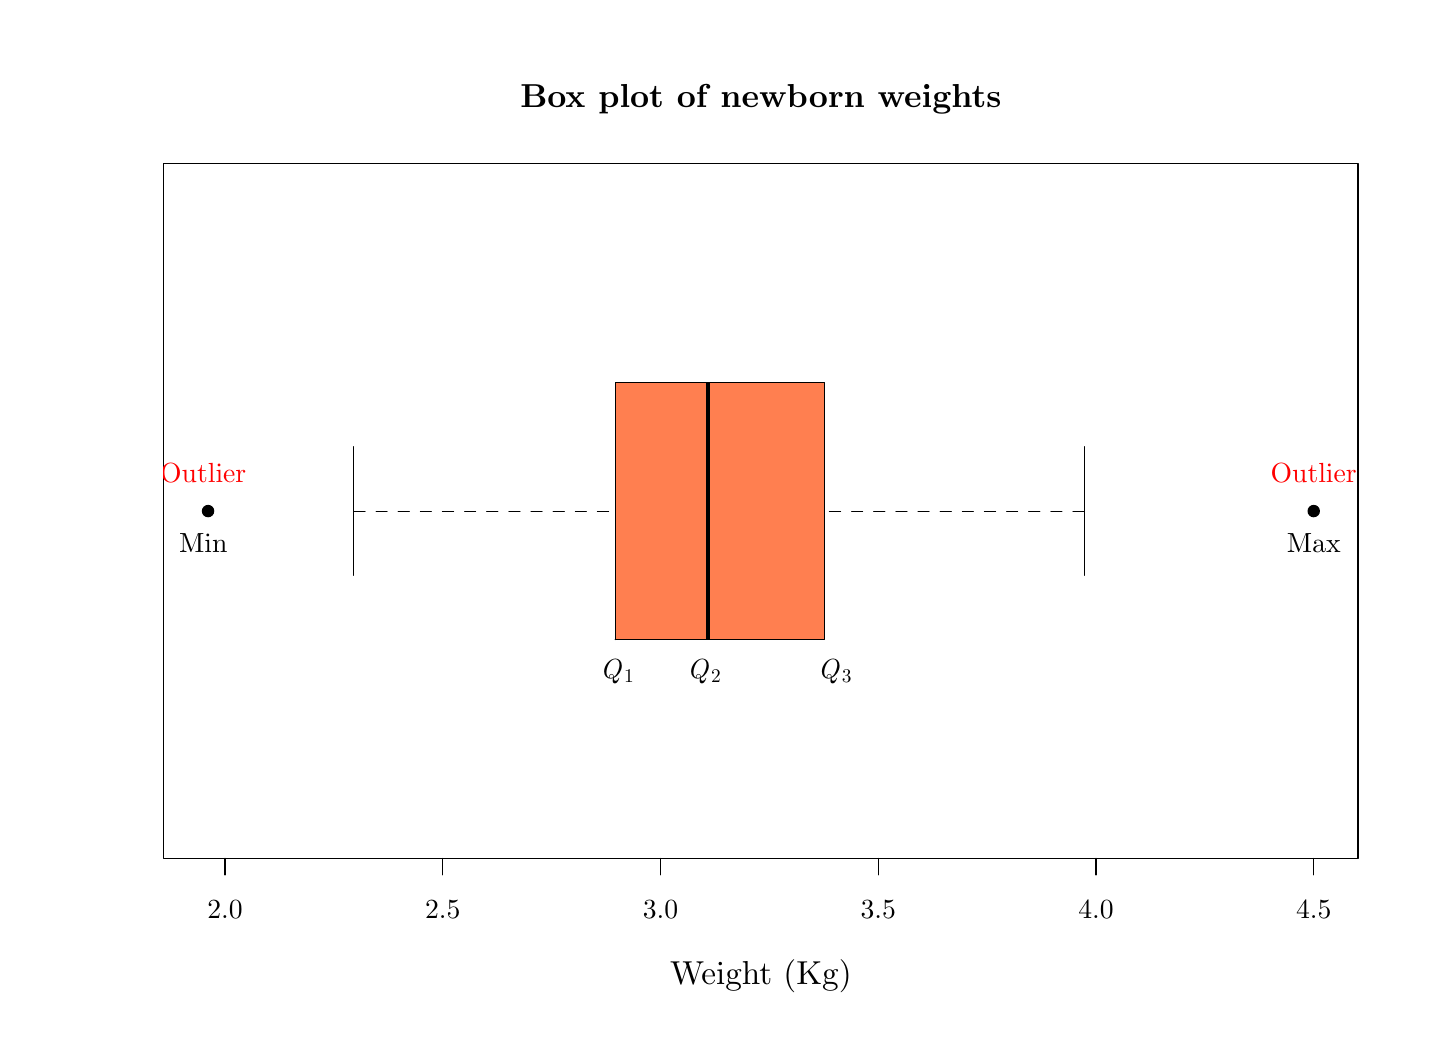
\begin{tikzpicture}[x=1pt,y=1pt]
\definecolor{fillColor}{RGB}{255,255,255}
\path[use as bounding box,fill=fillColor,fill opacity=0.00] (0,0) rectangle (505.89,361.35);
\begin{scope}
\path[clip] ( 49.20, 61.20) rectangle (480.69,312.15);
\definecolor{fillColor}{RGB}{255,127,80}

\path[fill=fillColor] (212.32,140.20) --
	(212.32,233.15) --
	(287.95,233.15) --
	(287.95,140.20) --
	cycle;
\definecolor{drawColor}{RGB}{0,0,0}

\path[draw=drawColor,line width= 1.2pt,line join=round] (245.85,140.20) -- (245.85,233.15);

\path[draw=drawColor,line width= 0.4pt,dash pattern=on 4pt off 4pt ,line join=round,line cap=round] (117.89,186.67) -- (212.32,186.67);

\path[draw=drawColor,line width= 0.4pt,dash pattern=on 4pt off 4pt ,line join=round,line cap=round] (381.73,186.67) -- (287.95,186.67);

\path[draw=drawColor,line width= 0.4pt,line join=round,line cap=round] (117.89,163.44) -- (117.89,209.91);

\path[draw=drawColor,line width= 0.4pt,line join=round,line cap=round] (381.73,163.44) -- (381.73,209.91);

\path[draw=drawColor,line width= 0.4pt,line join=round,line cap=round] (212.32,140.20) --
	(212.32,233.15) --
	(287.95,233.15) --
	(287.95,140.20) --
	(212.32,140.20);
\definecolor{fillColor}{RGB}{0,0,0}

\path[fill=fillColor] ( 65.18,186.67) circle (  2.25);

\path[fill=fillColor] (464.71,186.67) circle (  2.25);
\end{scope}
\begin{scope}
\path[clip] (  0.00,  0.00) rectangle (505.89,361.35);
\definecolor{drawColor}{RGB}{0,0,0}

\path[draw=drawColor,line width= 0.4pt,line join=round,line cap=round] ( 71.31, 61.20) -- (464.71, 61.20);

\path[draw=drawColor,line width= 0.4pt,line join=round,line cap=round] ( 71.31, 61.20) -- ( 71.31, 55.20);

\path[draw=drawColor,line width= 0.4pt,line join=round,line cap=round] (149.99, 61.20) -- (149.99, 55.20);

\path[draw=drawColor,line width= 0.4pt,line join=round,line cap=round] (228.67, 61.20) -- (228.67, 55.20);

\path[draw=drawColor,line width= 0.4pt,line join=round,line cap=round] (307.35, 61.20) -- (307.35, 55.20);

\path[draw=drawColor,line width= 0.4pt,line join=round,line cap=round] (386.03, 61.20) -- (386.03, 55.20);

\path[draw=drawColor,line width= 0.4pt,line join=round,line cap=round] (464.71, 61.20) -- (464.71, 55.20);

\node[text=drawColor,anchor=base,inner sep=0pt, outer sep=0pt, scale=  1.00] at ( 71.31, 39.60) {2.0};

\node[text=drawColor,anchor=base,inner sep=0pt, outer sep=0pt, scale=  1.00] at (149.99, 39.60) {2.5};

\node[text=drawColor,anchor=base,inner sep=0pt, outer sep=0pt, scale=  1.00] at (228.67, 39.60) {3.0};

\node[text=drawColor,anchor=base,inner sep=0pt, outer sep=0pt, scale=  1.00] at (307.35, 39.60) {3.5};

\node[text=drawColor,anchor=base,inner sep=0pt, outer sep=0pt, scale=  1.00] at (386.03, 39.60) {4.0};

\node[text=drawColor,anchor=base,inner sep=0pt, outer sep=0pt, scale=  1.00] at (464.71, 39.60) {4.5};
\end{scope}
\begin{scope}
\path[clip] (  0.00,  0.00) rectangle (505.89,361.35);
\definecolor{drawColor}{RGB}{0,0,0}

\node[text=drawColor,anchor=base,inner sep=0pt, outer sep=0pt, scale=  1.20] at (264.94,332.61) {\bfseries Box plot of newborn weights};

\node[text=drawColor,anchor=base,inner sep=0pt, outer sep=0pt, scale=  1.20] at (264.94, 15.60) {Weight (Kg)};
\end{scope}
\begin{scope}
\path[clip] (  0.00,  0.00) rectangle (505.89,361.35);
\definecolor{drawColor}{RGB}{0,0,0}

\path[draw=drawColor,line width= 0.4pt,line join=round,line cap=round] ( 49.20, 61.20) --
	(480.69, 61.20) --
	(480.69,312.15) --
	( 49.20,312.15) --
	( 49.20, 61.20);
\end{scope}
\begin{scope}
\path[clip] ( 49.20, 61.20) rectangle (480.69,312.15);
\definecolor{drawColor}{RGB}{0,0,0}

\node[text=drawColor,anchor=base west,inner sep=0pt, outer sep=0pt, scale=  1.00] at (206.83,126.11) {\itshape Q};

\node[text=drawColor,anchor=base west,inner sep=0pt, outer sep=0pt, scale=  0.70] at (215.53,124.61) {1};

\node[text=drawColor,anchor=base west,inner sep=0pt, outer sep=0pt, scale=  1.00] at (238.31,126.11) {\itshape Q};

\node[text=drawColor,anchor=base west,inner sep=0pt, outer sep=0pt, scale=  0.70] at (247.00,124.61) {2};

\node[text=drawColor,anchor=base west,inner sep=0pt, outer sep=0pt, scale=  1.00] at (285.51,126.11) {\itshape Q};

\node[text=drawColor,anchor=base west,inner sep=0pt, outer sep=0pt, scale=  0.70] at (294.21,124.61) {3};

\node[text=drawColor,anchor=base,inner sep=0pt, outer sep=0pt, scale=  1.00] at ( 63.44,171.61) {Min};

\node[text=drawColor,anchor=base,inner sep=0pt, outer sep=0pt, scale=  1.00] at (464.71,171.61) {Max};
\definecolor{drawColor}{RGB}{255,0,0}

\node[text=drawColor,anchor=base,inner sep=0pt, outer sep=0pt, scale=  1.00] at ( 63.44,197.17) {Outlier};

\node[text=drawColor,anchor=base,inner sep=0pt, outer sep=0pt, scale=  1.00] at (464.71,197.17) {Outlier};
\end{scope}
\end{tikzpicture}
}
\end{center}
\end{frame}


%---------------------------------------------------------------------slide----
\begin{frame}
\frametitle{Box plot construction}
To create a box plot follow the steps below
\begin{enumerate}
\item Calculate the quartiles. 
\item Draw a box from the lower to the upper quartile. 
\item Split the box with the median or second quartile. 
\item For the whiskers calculate first two values called \emph{fences}
\begin{align*}
f_1&=Q_1-1.5\,\text{IQR}\\
f_2&=Q_3+1.5\,\text{IQR}
\end{align*}
The fences define the interval where data are considered normal.
Any value outside that interval is considered an outlier. \\ 
For the lower whisker draw a segment from the lower quartile to the lower value in the sample grater than or
equal to $f_1$, and for the upper whisker draw a segment from the upper quartile to the highest value in the sample lower than
or equal to $f_2$.
\item Finally, if there are some outlier, draw a dot in every outlier. 
\end{enumerate}
\end{frame}


%---------------------------------------------------------------------slide----
\begin{frame}
\frametitle{Box plot construction}
\framesubtitle{Example of number of children}
\begin{enumerate}
\uncover<2->{\item Calculate the quartiles: $Q_1=1$ children} \uncover<3->{and $Q_2=Q_3=2$ children}
\uncover<4->{\item Draw the box.}
\uncover<5->{\item Calculate the fences $f_1=1-1.5*1=-0.5$ and $f_2=2+1.5*1=3.5$.}
\uncover<6->{\item Draw the whiskers: $w_1=0$ children} \uncover<7->{and $w_2=3$ children.}
\uncover<8->{\item Draw the outliers: 4 children.}
\end{enumerate}
\begin{center}
\tikzsetnextfilename{descriptive/boxplot_children}
\scalebox{0.45}{% Created by tikzDevice version 0.8.1 on 2015-11-15 21:50:56
% !TEX encoding = UTF-8 Unicode
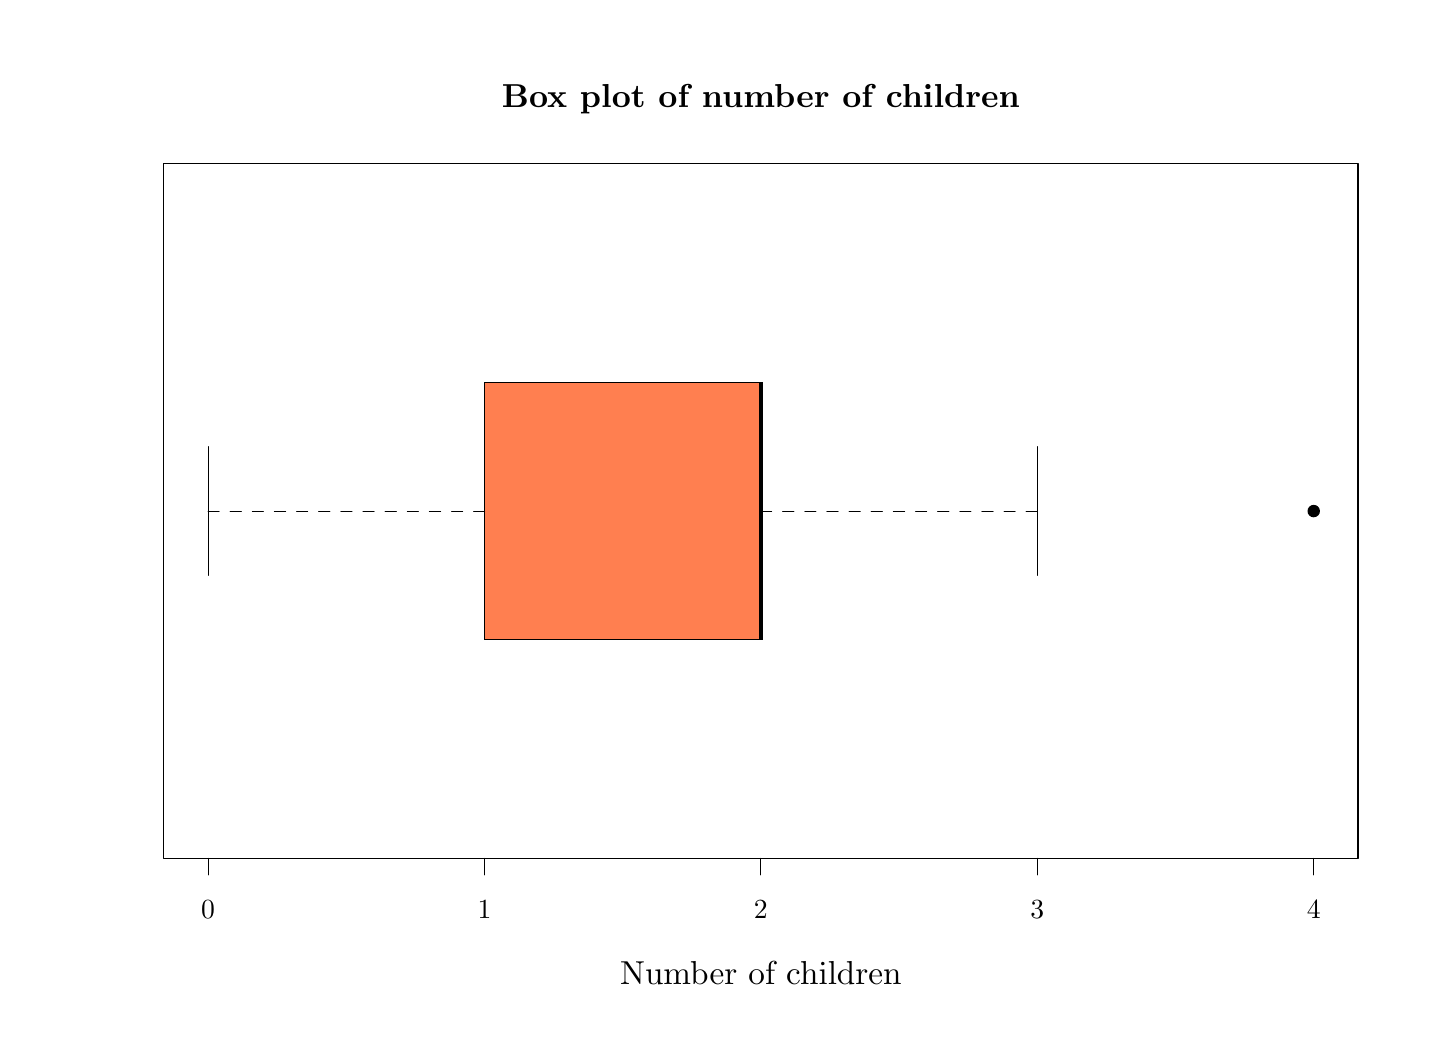
\begin{tikzpicture}[x=1pt,y=1pt]
\definecolor{fillColor}{RGB}{255,255,255}
\path[use as bounding box,fill=fillColor,fill opacity=0.00] (0,0) rectangle (505.89,361.35);
\path[draw,line width= 0.4pt,line join=round,line cap=round] ( 49.20, 61.20) --  (480.69, 61.20) --(480.69,312.15) -- (
49.20,312.15) -- ( 49.20, 61.20); 
\node[anchor=base,inner sep=0pt, outer sep=0pt, scale=  1.20] at (264.94,332.61) {\bfseries Box plot of number of children};
\node[anchor=base,inner sep=0pt, outer sep=0pt, scale=  1.20] at (264.94, 15.60) {Number of children};
\path[draw,line width= 0.4pt,line join=round,line cap=round] ( 65.18, 61.20) -- (464.71, 61.20);
\path[draw,line width= 0.4pt,line join=round,line cap=round] ( 65.18, 61.20) -- ( 65.18, 55.20);
\path[draw,line width= 0.4pt,line join=round,line cap=round] (165.06, 61.20) -- (165.06, 55.20);
\path[draw,line width= 0.4pt,line join=round,line cap=round] (264.94, 61.20) -- (264.94, 55.20);
\path[draw,line width= 0.4pt,line join=round,line cap=round] (364.83, 61.20) -- (364.83, 55.20);
\path[draw,line width= 0.4pt,line join=round,line cap=round] (464.71, 61.20) -- (464.71, 55.20);
\node[anchor=base,inner sep=0pt, outer sep=0pt, scale=  1.00] at ( 65.18, 39.60) {0};
\node[anchor=base,inner sep=0pt, outer sep=0pt, scale=  1.00] at (165.06, 39.60) {1};
\node[anchor=base,inner sep=0pt, outer sep=0pt, scale=  1.00] at (264.94, 39.60) {2};
\node[anchor=base,inner sep=0pt, outer sep=0pt, scale=  1.00] at (364.83, 39.60) {3};
\node[anchor=base,inner sep=0pt, outer sep=0pt, scale=  1.00] at (464.71, 39.60) {4};
\begin{scope}
\path[clip] ( 49.20, 61.20) rectangle (480.69,312.15);
\pause
\definecolor{fillColor}{RGB}{255,127,80}
\path[draw] (165.06,140.20) -- (165.06,233.15);
\pause
\path[draw] (264.94,233.15) --	(264.94,140.20);
\pause
\path[draw, fill=fillColor] (165.06,140.20) -- (165.06,233.15) --	(264.94,233.15) --	(264.94,140.20) --	cycle;
\path[draw,line width= 1.2pt,line join=round] (264.94,140.20) -- (264.94,233.15);
\pause
\pause
\path[draw,line width= 0.4pt,line join=round,line cap=round] ( 65.18,163.44) -- ( 65.18,209.91);
\path[draw,line width= 0.4pt,dash pattern=on 4pt off 4pt ,line join=round,line cap=round] ( 65.18,186.67) -- (165.06,186.67);
\pause
\path[draw,line width= 0.4pt,dash pattern=on 4pt off 4pt ,line join=round,line cap=round] (364.83,186.67) -- (264.94,186.67);
\path[draw,line width= 0.4pt,line join=round,line cap=round] (364.83,163.44) -- (364.83,209.91);
\pause
\path[fill] (464.71,186.67) circle (  2.25);
\end{scope}
\pause
\end{tikzpicture}
}
\end{center}
\end{frame}


%---------------------------------------------------------------------slide----
\begin{frame}
\frametitle{Deviations from the mean}
Another way of measuring spread of data is with respect to a central tendency measure, as for example the mean. 

In that case, it's measured the distance from every value in the sample to the mean, that is called
\highlight{\textbf{deviation from the mean.}}

\begin{center}
\tikzsetnextfilename{descriptive/deviations}
\scalebox{1}{% Author: Alfredo Sánchez Alberca (email:asalber@ceu.es)
% Plot with the interquartile range
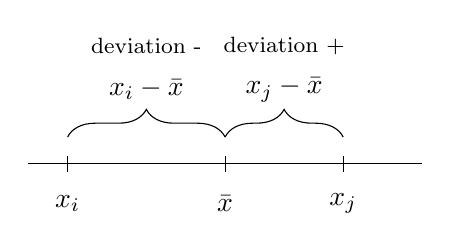
\begin{tikzpicture}[every label/.style={text=color1}]
\draw (0,1) -- (5,1);
\draw (2.5,0.9) -- (2.5,1.1);
\node at (2.5,0.5) {$\bar x$};
\draw (0.5,0.9) -- (0.5,1.1);
\node at (0.5,0.5) {$x_i$}; 
\draw (4,0.9) -- (4,1.1);
\node at (4,0.5) {$x_j$};  
\draw [decorate,decoration={brace,amplitude=10pt},yshift=4pt] (0.5,1.2) -- (2.5,1.2) node
[black,midway,yshift=0.6cm] {$x_i-\bar x$};
\draw [decorate,decoration={brace,amplitude=10pt},yshift=4pt] (2.5,1.2) -- (4,1.2) node
[black,midway,yshift=0.6cm] {$x_j-\bar x$};
\node at (1.5,2.5) {\footnotesize deviation -};
\node at (3.25,2.5) {\footnotesize deviation +};
\end{tikzpicture}}
\end{center}

If deviations are big, the mean is less representative than when they are small.
%\begin{center} 
%\emph{Which mean is more representative?}
%\end{center}
\end{frame}


%---------------------------------------------------------------------slide----
\begin{frame}
\frametitle{Variance and standard deviation}
\begin{definition}[Sample variance $s^2$]
The \emph{sample variance} of a variable $X$ is the average of squared deviations from the mean. 
\[
s^2 = \frac{\sum (x_i-\bar x)^2n_i}{n} = \sum (x_i-\bar x)^2f_i
\]
\end{definition}
It can also be calculated with the formula
\[
s^2 = \frac{\sum x_i^2n_i}{n} -\bar x^2= \sum x_i^2f_i-\bar x^2
\]
The variance has the units of the variable squared, and to ease their interpretation it's common to calculate its square
root.

\begin{definition}[Sample standard deviation $s$]
The \emph{sample standard deviation} of a variable $X$ is the square root of the variance.
\[
s = +\sqrt{s^2}
\]
\end{definition}
\end{frame}


%---------------------------------------------------------------------slide----
\begin{frame}
\frametitle{Variance and standard deviation interpretation}
Both variance and standard deviation measures the spread of data around the mean. 
When the variance or the standard deviation are small, the sample data are concentrated around the mean, and the mean is
a good representative measure. 
In contrast, when variance or the standard deviation are high, the sample data are far from the mean, and the mean
doesn't represent so good. 
\begin{center}
\begin{tabular}{lcl}
\emph{Standard deviation small} & $\Rightarrow$ & \emph{Mean is representative}\\
\emph{Standard deviation big} & $\Rightarrow$ & \emph{Mean is unrepresentative}\\
\end{tabular}
\end{center}

\highlight{\textbf{Example}} The following samples contains the grades of 2 students in 2 subjects 
\begin{center}
\tikzsetnextfilename{descriptive/std_deviation_interpretation}
\scalebox{1}{% Author: Alfredo Sánchez Alberca (email:asalber@ceu.es)
% Plot with the interquartile range
\begin{tikzpicture}
\draw (0,2) -- (5,2);
\draw[color=color1] (2.5,1.9) -- (2.5,2.1);
\node[text=color1] at (2.5,2.3) {$\bar x$};
\node[text=color1] at (2.5,1.7) {$5$};
\draw (0.5,1.9) -- (0.5,2.1);
\node at (0.5,1.7) {$1$}; 
\draw (4.5,1.9) -- (4.5,2.1);
\node at (4.5,1.7) {$9$};  
\node at (-1,2) {Student 1};
\node at (5.5,2) {$s=4$};
\pause
\draw (0,1) -- (5,1);
\draw[color=color1] (2.5,0.9) -- (2.5,1.1);
\node[text=color1] at (2.5,1.3) {$\bar x$};
\draw (2,0.9) -- (2,1.1);
\node at (2,0.7) {$4$}; 
\draw (3,0.9) -- (3,1.1);
\node at (3,0.7) {$6$};  
\node[text=color1] at (2.5,0.7) {$5$};
\node at (-1,1) {Student 2};
\node at (5.5,1) {$s=1$};
\end{tikzpicture}}

\uncover<2->{\emph{Which mean is more representative?}}
\end{center}
\end{frame}


%---------------------------------------------------------------------slide----
\begin{frame}
\frametitle{Variance and standard deviation calculation}
\framesubtitle{Example with non-grouped data}
Using the data of the sample with the number of children of families, and adding a new column to the frequency table
with the squared values, 
\[
\setlength\arraycolsep{3mm}
\setlength\arrayrulewidth{0.5pt}
\begin{array}{rrr}
\hline
\multicolumn{1}{c}{x_i} & \multicolumn{1}{c}{f_i} & \multicolumn{1}{c}{x_i^2f_i} \\
\hline
0 & 0.08 & 0.00 \\
1 & 0.24 & 0.24 \\
2 & 0.56 & 2.24\\
3 & 0.08  & 0.72\\
4 & 0.04 & 0.64 \\
\hline
\sum &  &  3.84\\ 
\hline
\end{array}
\]
\[
s^2 = \sum x_i^2f_i-\bar x^2 = 3.84-1.76^2= 0.7424 \mbox{ children}^2,
\]
and the standard deviation is $s=\sqrt{0.7424} = 0.8616$ children.

Compared to the range, that is 4 children, the standard deviation is not very large, so we can conclude
that the dispersion of the distribution is small and consequently the mean, $\bar x=1.76$ children, represents quite
well the number of children of families of the sample. 
\end{frame}


%---------------------------------------------------------------------slide----
\begin{frame}
\frametitle{Variance and standard deviation calculation}
\framesubtitle{Example with grouped data}
Using the data of the sample with the heights of students and grouping heights in classes, the calculation is the same
but using the class marks. 

\[
\setlength\arraycolsep{3mm}
\setlength\arrayrulewidth{0.5pt}
\begin{array}{rrrr}
\hline
\multicolumn{1}{c}{X} & \multicolumn{1}{c}{x_i} & \multicolumn{1}{c}{n_i} & \multicolumn{1}{c}{x_i^2n_i} \\
\hline
(150,160] & 155 & 2 & 48050\\
(160,170] & 165 & 8 & 217800\\
(170,180] & 175 & 11 & 336875\\
(180,190] & 185 & 7 & 239575\\
(190,200] & 195 & 2 & 76050\\
\hline
\sum &  & 30 & 918350 \\
\hline
\end{array}
\]
\[
s^2 = \frac{\sum x_i^2n_i}{n}-\bar x^2 = \frac{918350}{30}-174.67^2= 102.06 \mbox{ cm}^2,
\]
and the standard deviation is $s=\sqrt{102.06} = 10.1$ cm.

This value is quite small compared to the range of the variable, that goes from 150 to 200 cm, therefore the
distribution of heights has little dispersion and the mean is very representative.
\end{frame}


%---------------------------------------------------------------------slide----
\begin{frame}
\frametitle{Coefficient of variation}
Both, variance and standard deviation, have units and that makes difficult to interpret them, specially when comparing
distributions of variables with different units.

For that reason it's also common to use the following dispersion measure that has no units.  
\begin{definition}[Sample coefficient of variation $cv$]
The \emph{sample coefficient of variation} of a variable $X$ is the quotient between the sample standard deviation and se
absolute value of the sample mean.
\[
cv = \frac{s}{|\bar x|}
\]
\end{definition}
The coefficient of variation measures the relative dispersion of data around the sample mean.  

As it has no units, it's easier to interpret: The higher the it is the higher the relative dispersion with respect to
the mean and less representative is the mean.

The coefficient of variation it's very helpful to compare dispersion in distributions of different variables, even if
variables have different units.
\begin{center}
\alert{\emph{Watch out! It makes no sense when the mean is 0 or close to 0.}}
\end{center}
\end{frame}


%---------------------------------------------------------------------slide----
\begin{frame}
\frametitle{Coefficient of variation}
\framesubtitle{Example}
In the sample of the number of children, where the mean was $\bar x=1.76$ and the standard deviation was $s=0.8616$
children, the coefficient of variation is
\[
cv = \frac{s}{|\bar x|} = \frac{0.8616}{|1.76|} = 0.49.
\]
In the sample of heights, where the mean was $\bar x=174.67$ cm and the standard deviation was $s=10.1$ cm, the
coefficient of variation is
\[
cv = \frac{s}{|\bar x|} = \frac{10.1}{|174.67|} = 0.06.
\]

This means that the relative dispersion in the heights distribution is lower than in the number of children
distribution, and consequently the mean of height is most representative than the mean of number of children.
\end{frame}


\subsection{Shape statistics}
%---------------------------------------------------------------------slide----
\begin{frame}
\frametitle{Shape statistics}
They are measures that describe the shape of the distribution. 

In particular, the most important aspects are:
\begin{description}
\item[Symmetry:] It measures the symmetry of the distribution with respect to the mean. \\
The statistics most used is the \emph{coefficient of skewness}.
\item[Kurtosis:] It measures the length of tails or the peakness of distribution. \\
The statistics most used is the \emph{coefficient of kurtosis}.
\end{description}
\end{frame}


%---------------------------------------------------------------------slide----
\begin{frame}
\frametitle{Coefficient of skewness}
\begin{definition}[Sample coefficient of skewness $g_1$]
The \emph{sample coefficient of skewness} of a variable $X$ is the average of the deviations of values from the sample
mean to cube, divided by the standard deviation to cube. 
\[
g_1 = \frac{\sum (x_i-\bar x)^3 n_i/n}{s^3} = \frac{\sum (x_i-\bar x)^3 f_i}{s^3}
\]
\end{definition}

It measures the symmetry or skewness of the distribution, that is, how many values in the
sample are above or below the mean and how far from it. 
\begin{itemize}
\item $g_1=0$ indicates that there are the same number of values in the sample above and below the mean and
equally deviated from it, and the distribution is symmetrical.
\item $g_1<0$ indicates that there are more values above the mean than below it, but the values below are further from
it, and the distribution is left-skewed (it has longer tail to the left). 
\item $g_1>0$ indicates that there are more values below the mean than above it, but the values above are further from
it, and the distribution is right-skewed (it has longer tail to the right).  
\end{itemize}
\end{frame}


%---------------------------------------------------------------------slide----
\begin{frame}
\frametitle{Coefficient of skewness}
\framesubtitle{Example of symmetrical distribution}
\begin{center}
\tikzsetnextfilename{descriptive/symmetrical_distribution}
\scalebox{0.6}{% Created by tikzDevice version 0.9 on 2015-11-20 12:10:21
% !TEX encoding = UTF-8 Unicode
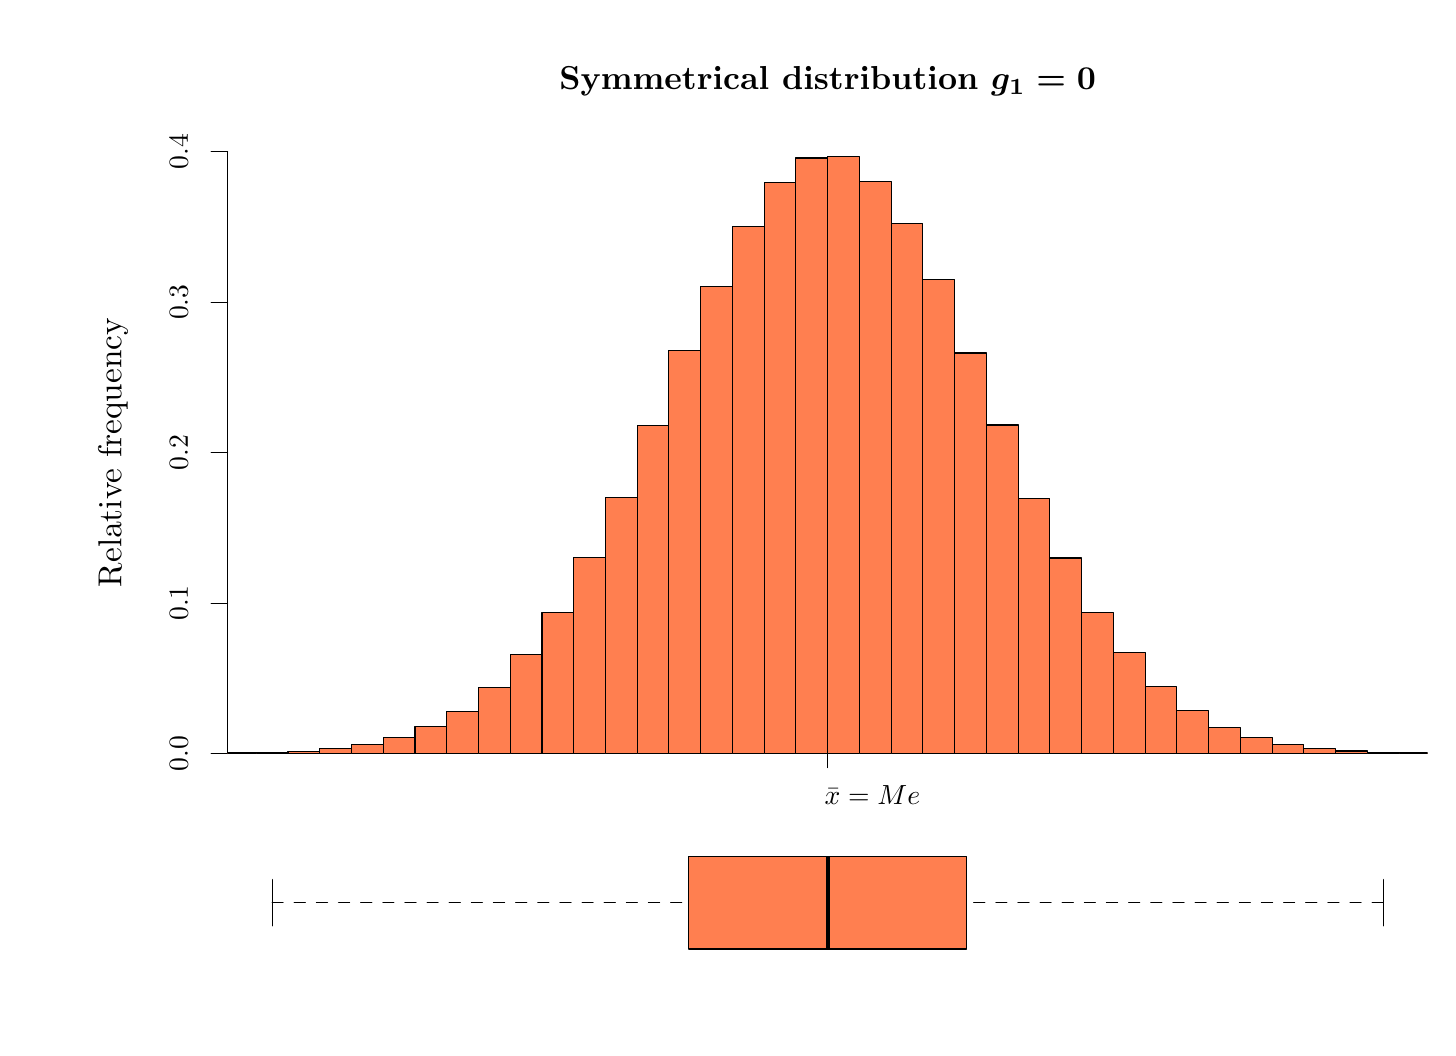
\begin{tikzpicture}[x=1pt,y=1pt]
\definecolor{fillColor}{RGB}{255,255,255}
\path[use as bounding box,fill=fillColor,fill opacity=0.00] (0,0) rectangle (505.89,361.35);
\begin{scope}
\path[clip] (  0.00, 90.34) rectangle (505.89,361.35);
\definecolor{drawColor}{RGB}{0,0,0}

\node[text=drawColor,anchor=base,inner sep=0pt, outer sep=0pt, scale=  1.20, font=\boldmath] at (289.08,339.14)
{\bfseries Symmetrical distribution $g_1=0$};
 
\node[text=drawColor,rotate= 90.00,anchor=base,inner sep=0pt, outer sep=0pt, scale=  1.20] at ( 33.87,207.78) {Relative frequency};
\end{scope}
\begin{scope}
\path[clip] (  0.00,  0.00) rectangle (505.89,361.35);
\definecolor{drawColor}{RGB}{0,0,0}

\path[draw=drawColor,line width= 0.4pt,line join=round,line cap=round] ( 72.27, 99.04) -- ( 72.27,316.52);

\path[draw=drawColor,line width= 0.4pt,line join=round,line cap=round] ( 72.27, 99.04) -- ( 66.27, 99.04);

\path[draw=drawColor,line width= 0.4pt,line join=round,line cap=round] ( 72.27,153.41) -- ( 66.27,153.41);

\path[draw=drawColor,line width= 0.4pt,line join=round,line cap=round] ( 72.27,207.78) -- ( 66.27,207.78);

\path[draw=drawColor,line width= 0.4pt,line join=round,line cap=round] ( 72.27,262.15) -- ( 66.27,262.15);

\path[draw=drawColor,line width= 0.4pt,line join=round,line cap=round] ( 72.27,316.52) -- ( 66.27,316.52);

\node[text=drawColor,rotate= 90.00,anchor=base,inner sep=0pt, outer sep=0pt, scale=  1.00] at ( 57.87, 99.04) {0.0};

\node[text=drawColor,rotate= 90.00,anchor=base,inner sep=0pt, outer sep=0pt, scale=  1.00] at ( 57.87,153.41) {0.1};

\node[text=drawColor,rotate= 90.00,anchor=base,inner sep=0pt, outer sep=0pt, scale=  1.00] at ( 57.87,207.78) {0.2};

\node[text=drawColor,rotate= 90.00,anchor=base,inner sep=0pt, outer sep=0pt, scale=  1.00] at ( 57.87,262.15) {0.3};

\node[text=drawColor,rotate= 90.00,anchor=base,inner sep=0pt, outer sep=0pt, scale=  1.00] at ( 57.87,316.52) {0.4};
\end{scope}
\begin{scope}
\path[clip] ( 72.27, 90.34) rectangle (505.89,325.21);
\definecolor{drawColor}{RGB}{0,0,0}
\definecolor{fillColor}{RGB}{255,127,80}

\path[draw=drawColor,line width= 0.4pt,line join=round,line cap=round,fill=fillColor] ( 13.77, 99.04) rectangle ( 25.24, 99.04);

\path[draw=drawColor,line width= 0.4pt,line join=round,line cap=round,fill=fillColor] ( 25.24, 99.04) rectangle ( 36.71, 99.05);

\path[draw=drawColor,line width= 0.4pt,line join=round,line cap=round,fill=fillColor] ( 36.71, 99.04) rectangle ( 48.18, 99.06);

\path[draw=drawColor,line width= 0.4pt,line join=round,line cap=round,fill=fillColor] ( 48.18, 99.04) rectangle ( 59.65, 99.09);

\path[draw=drawColor,line width= 0.4pt,line join=round,line cap=round,fill=fillColor] ( 59.65, 99.04) rectangle ( 71.12, 99.16);

\path[draw=drawColor,line width= 0.4pt,line join=round,line cap=round,fill=fillColor] ( 71.12, 99.04) rectangle ( 82.59, 99.30);

\path[draw=drawColor,line width= 0.4pt,line join=round,line cap=round,fill=fillColor] ( 82.59, 99.04) rectangle ( 94.07, 99.52);

\path[draw=drawColor,line width= 0.4pt,line join=round,line cap=round,fill=fillColor] ( 94.07, 99.04) rectangle (105.54, 99.95);

\path[draw=drawColor,line width= 0.4pt,line join=round,line cap=round,fill=fillColor] (105.54, 99.04) rectangle (117.01,100.89);

\path[draw=drawColor,line width= 0.4pt,line join=round,line cap=round,fill=fillColor] (117.01, 99.04) rectangle (128.48,102.31);

\path[draw=drawColor,line width= 0.4pt,line join=round,line cap=round,fill=fillColor] (128.48, 99.04) rectangle (139.95,104.82);

\path[draw=drawColor,line width= 0.4pt,line join=round,line cap=round,fill=fillColor] (139.95, 99.04) rectangle (151.42,108.79);

\path[draw=drawColor,line width= 0.4pt,line join=round,line cap=round,fill=fillColor] (151.42, 99.04) rectangle (162.89,114.39);

\path[draw=drawColor,line width= 0.4pt,line join=round,line cap=round,fill=fillColor] (162.89, 99.04) rectangle (174.37,123.01);

\path[draw=drawColor,line width= 0.4pt,line join=round,line cap=round,fill=fillColor] (174.37, 99.04) rectangle (185.84,134.71);

\path[draw=drawColor,line width= 0.4pt,line join=round,line cap=round,fill=fillColor] (185.84, 99.04) rectangle (197.31,150.13);

\path[draw=drawColor,line width= 0.4pt,line join=round,line cap=round,fill=fillColor] (197.31, 99.04) rectangle (208.78,169.74);

\path[draw=drawColor,line width= 0.4pt,line join=round,line cap=round,fill=fillColor] (208.78, 99.04) rectangle (220.25,191.61);

\path[draw=drawColor,line width= 0.4pt,line join=round,line cap=round,fill=fillColor] (220.25, 99.04) rectangle (231.72,217.53);

\path[draw=drawColor,line width= 0.4pt,line join=round,line cap=round,fill=fillColor] (231.72, 99.04) rectangle (243.19,244.61);

\path[draw=drawColor,line width= 0.4pt,line join=round,line cap=round,fill=fillColor] (243.19, 99.04) rectangle (254.67,267.97);

\path[draw=drawColor,line width= 0.4pt,line join=round,line cap=round,fill=fillColor] (254.67, 99.04) rectangle (266.14,289.65);

\path[draw=drawColor,line width= 0.4pt,line join=round,line cap=round,fill=fillColor] (266.14, 99.04) rectangle (277.61,305.28);

\path[draw=drawColor,line width= 0.4pt,line join=round,line cap=round,fill=fillColor] (277.61, 99.04) rectangle (289.08,314.26);

\path[draw=drawColor,line width= 0.4pt,line join=round,line cap=round,fill=fillColor] (289.08, 99.04) rectangle (300.55,314.91);

\path[draw=drawColor,line width= 0.4pt,line join=round,line cap=round,fill=fillColor] (300.55, 99.04) rectangle (312.02,305.72);

\path[draw=drawColor,line width= 0.4pt,line join=round,line cap=round,fill=fillColor] (312.02, 99.04) rectangle (323.49,290.70);

\path[draw=drawColor,line width= 0.4pt,line join=round,line cap=round,fill=fillColor] (323.49, 99.04) rectangle (334.97,270.37);

\path[draw=drawColor,line width= 0.4pt,line join=round,line cap=round,fill=fillColor] (334.97, 99.04) rectangle (346.44,243.80);

\path[draw=drawColor,line width= 0.4pt,line join=round,line cap=round,fill=fillColor] (346.44, 99.04) rectangle (357.91,217.79);

\path[draw=drawColor,line width= 0.4pt,line join=round,line cap=round,fill=fillColor] (357.91, 99.04) rectangle (369.38,191.33);

\path[draw=drawColor,line width= 0.4pt,line join=round,line cap=round,fill=fillColor] (369.38, 99.04) rectangle (380.85,169.70);

\path[draw=drawColor,line width= 0.4pt,line join=round,line cap=round,fill=fillColor] (380.85, 99.04) rectangle (392.32,150.03);

\path[draw=drawColor,line width= 0.4pt,line join=round,line cap=round,fill=fillColor] (392.32, 99.04) rectangle (403.79,135.51);

\path[draw=drawColor,line width= 0.4pt,line join=round,line cap=round,fill=fillColor] (403.79, 99.04) rectangle (415.27,123.17);

\path[draw=drawColor,line width= 0.4pt,line join=round,line cap=round,fill=fillColor] (415.27, 99.04) rectangle (426.74,114.54);

\path[draw=drawColor,line width= 0.4pt,line join=round,line cap=round,fill=fillColor] (426.74, 99.04) rectangle (438.21,108.56);

\path[draw=drawColor,line width= 0.4pt,line join=round,line cap=round,fill=fillColor] (438.21, 99.04) rectangle (449.68,104.81);

\path[draw=drawColor,line width= 0.4pt,line join=round,line cap=round,fill=fillColor] (449.68, 99.04) rectangle (461.15,102.37);

\path[draw=drawColor,line width= 0.4pt,line join=round,line cap=round,fill=fillColor] (461.15, 99.04) rectangle (472.62,100.87);

\path[draw=drawColor,line width= 0.4pt,line join=round,line cap=round,fill=fillColor] (472.62, 99.04) rectangle (484.09, 99.97);

\path[draw=drawColor,line width= 0.4pt,line join=round,line cap=round,fill=fillColor] (484.09, 99.04) rectangle (495.57, 99.57);

\path[draw=drawColor,line width= 0.4pt,line join=round,line cap=round,fill=fillColor] (495.57, 99.04) rectangle (507.04, 99.27);
\end{scope}
\begin{scope}
\path[clip] (  0.00,  0.00) rectangle (505.89,361.35);
\definecolor{drawColor}{RGB}{0,0,0}

\path[draw=drawColor,line width= 0.4pt,line join=round,line cap=round] (289.15, 99.04) -- (289.15, 94);

\node[text=drawColor,anchor=west,inner sep=0pt, outer sep=0pt, scale=  1.00] at (288, 84) {$\bar x=Me$};
\end{scope}
\begin{scope}
\path[clip] ( 72.27,  0.00) rectangle (505.89, 90.34);
\definecolor{fillColor}{RGB}{255,127,80}

\path[fill=fillColor] (238.87, 28.44) --
	(238.87, 61.90) --
	(339.25, 61.90) --
	(339.25, 28.44) --
	cycle;
\definecolor{drawColor}{RGB}{0,0,0}

\path[draw=drawColor,line width= 1.2pt,line join=round] (289.15, 28.44) -- (289.15, 61.90);

\path[draw=drawColor,line width= 0.4pt,dash pattern=on 4pt off 4pt ,line join=round,line cap=round] ( 88.33, 45.17) -- (238.87, 45.17);

\path[draw=drawColor,line width= 0.4pt,dash pattern=on 4pt off 4pt ,line join=round,line cap=round] (489.83, 45.17) -- (339.25, 45.17);

\path[draw=drawColor,line width= 0.4pt,line join=round,line cap=round] ( 88.33, 36.80) -- ( 88.33, 53.53);

\path[draw=drawColor,line width= 0.4pt,line join=round,line cap=round] (489.83, 36.80) -- (489.83, 53.53);

\path[draw=drawColor,line width= 0.4pt,line join=round,line cap=round] (238.87, 28.44) --
	(238.87, 61.90) --
	(339.25, 61.90) --
	(339.25, 28.44) --
	(238.87, 28.44);
\end{scope}
\end{tikzpicture}
}
\end{center}
\end{frame} 


%---------------------------------------------------------------------slide----
\begin{frame}
\frametitle{Coefficient of skewness}
\framesubtitle{Example of left-skewed distribution}
\begin{center}
\tikzsetnextfilename{descriptive/left_skewed_distribution}
\scalebox{0.6}{% Created by tikzDevice version 0.9 on 2015-11-20 12:13:52
% !TEX encoding = UTF-8 Unicode
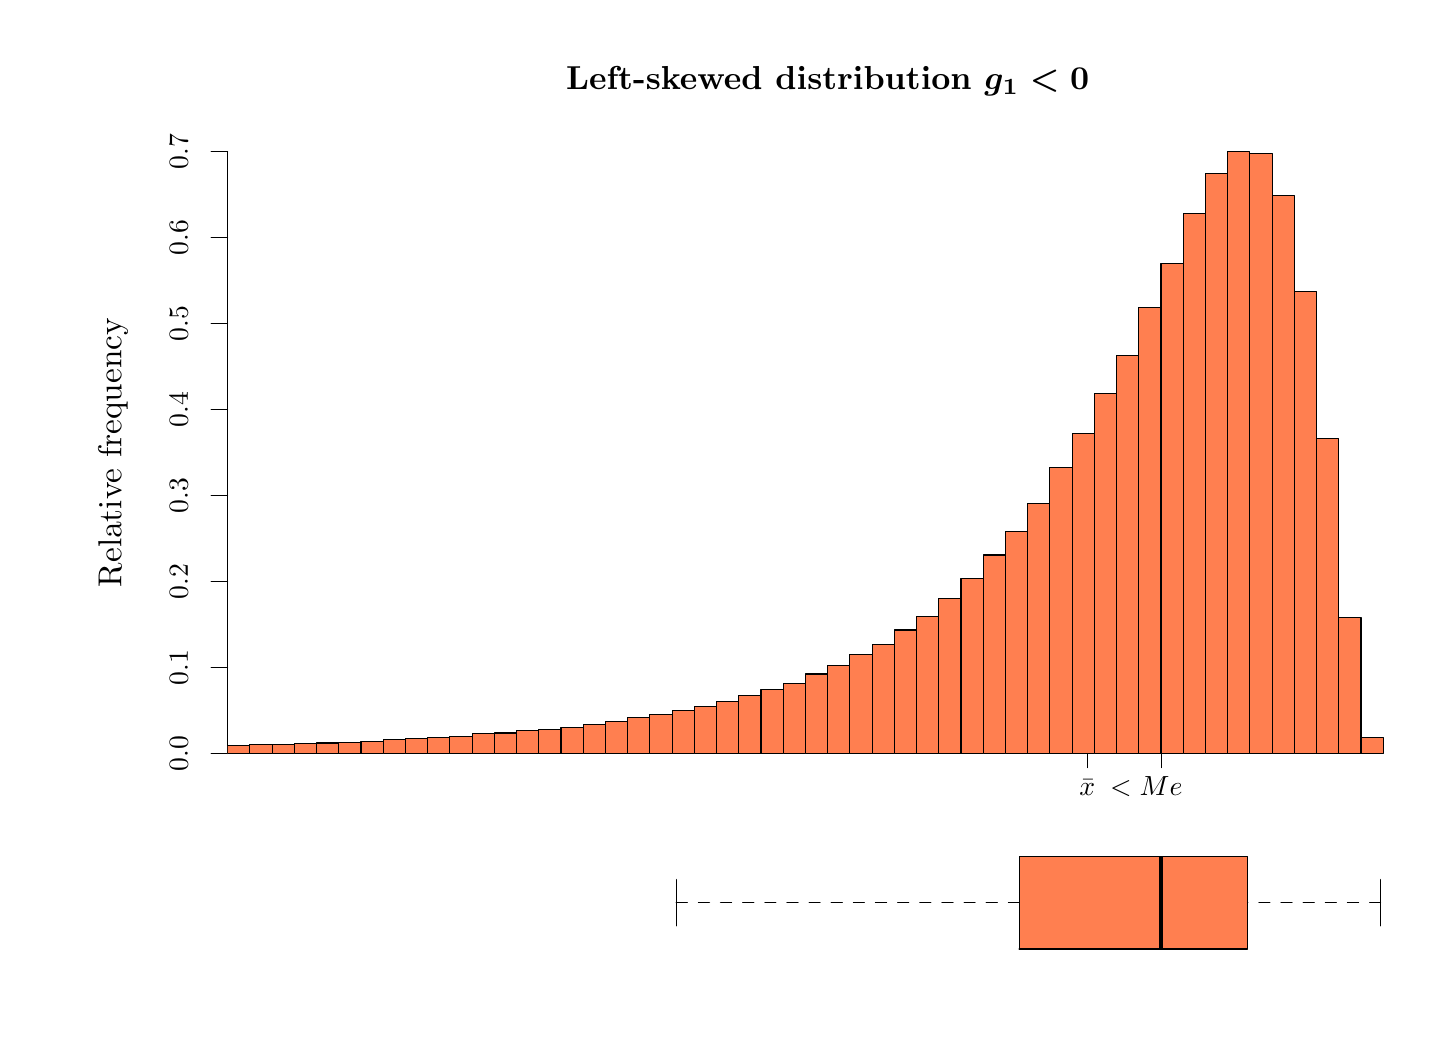
\begin{tikzpicture}[x=1pt,y=1pt]
\definecolor{fillColor}{RGB}{255,255,255}
\path[use as bounding box,fill=fillColor,fill opacity=0.00] (0,0) rectangle (505.89,361.35);
\begin{scope}
\path[clip] (  0.00, 90.34) rectangle (505.89,361.35);
\definecolor{drawColor}{RGB}{0,0,0}

\node[text=drawColor,anchor=base,inner sep=0pt, outer sep=0pt, scale=  1.20, font=\boldmath] at (289.08,339.14)
{\bfseries Left-skewed distribution $g_1<0$};

\node[text=drawColor,anchor=base,inner sep=0pt, outer sep=0pt, scale=  1.20] at (289.08, 44.74) {-x};

\node[text=drawColor,rotate= 90.00,anchor=base,inner sep=0pt, outer sep=0pt, scale=  1.20] at ( 33.87,207.78) {Relative frequency};
\end{scope}
\begin{scope}
\path[clip] (  0.00,  0.00) rectangle (505.89,361.35);
\definecolor{drawColor}{RGB}{0,0,0}

\path[draw=drawColor,line width= 0.4pt,line join=round,line cap=round] ( 72.27, 99.04) -- ( 72.27,316.56);

\path[draw=drawColor,line width= 0.4pt,line join=round,line cap=round] ( 72.27, 99.04) -- ( 66.27, 99.04);

\path[draw=drawColor,line width= 0.4pt,line join=round,line cap=round] ( 72.27,130.11) -- ( 66.27,130.11);

\path[draw=drawColor,line width= 0.4pt,line join=round,line cap=round] ( 72.27,161.19) -- ( 66.27,161.19);

\path[draw=drawColor,line width= 0.4pt,line join=round,line cap=round] ( 72.27,192.26) -- ( 66.27,192.26);

\path[draw=drawColor,line width= 0.4pt,line join=round,line cap=round] ( 72.27,223.33) -- ( 66.27,223.33);

\path[draw=drawColor,line width= 0.4pt,line join=round,line cap=round] ( 72.27,254.41) -- ( 66.27,254.41);

\path[draw=drawColor,line width= 0.4pt,line join=round,line cap=round] ( 72.27,285.48) -- ( 66.27,285.48);

\path[draw=drawColor,line width= 0.4pt,line join=round,line cap=round] ( 72.27,316.56) -- ( 66.27,316.56);

\node[text=drawColor,rotate= 90.00,anchor=base,inner sep=0pt, outer sep=0pt, scale=  1.00] at ( 57.87, 99.04) {0.0};

\node[text=drawColor,rotate= 90.00,anchor=base,inner sep=0pt, outer sep=0pt, scale=  1.00] at ( 57.87,130.11) {0.1};

\node[text=drawColor,rotate= 90.00,anchor=base,inner sep=0pt, outer sep=0pt, scale=  1.00] at ( 57.87,161.19) {0.2};

\node[text=drawColor,rotate= 90.00,anchor=base,inner sep=0pt, outer sep=0pt, scale=  1.00] at ( 57.87,192.26) {0.3};

\node[text=drawColor,rotate= 90.00,anchor=base,inner sep=0pt, outer sep=0pt, scale=  1.00] at ( 57.87,223.33) {0.4};

\node[text=drawColor,rotate= 90.00,anchor=base,inner sep=0pt, outer sep=0pt, scale=  1.00] at ( 57.87,254.41) {0.5};

\node[text=drawColor,rotate= 90.00,anchor=base,inner sep=0pt, outer sep=0pt, scale=  1.00] at ( 57.87,285.48) {0.6};

\node[text=drawColor,rotate= 90.00,anchor=base,inner sep=0pt, outer sep=0pt, scale=  1.00] at ( 57.87,316.56) {0.7};
\end{scope}
\begin{scope}
\path[clip] ( 72.27, 90.34) rectangle (505.89,325.21);
\definecolor{drawColor}{RGB}{0,0,0}
\definecolor{fillColor}{RGB}{255,127,80}

\path[draw=drawColor,line width= 0.4pt,line join=round,line cap=round,fill=fillColor] ( -8.03, 99.04) rectangle (  0.00,100.53);

\path[draw=drawColor,line width= 0.4pt,line join=round,line cap=round,fill=fillColor] (  0.00, 99.04) rectangle (  8.03,100.54);

\path[draw=drawColor,line width= 0.4pt,line join=round,line cap=round,fill=fillColor] (  8.03, 99.04) rectangle ( 16.06,100.72);

\path[draw=drawColor,line width= 0.4pt,line join=round,line cap=round,fill=fillColor] ( 16.06, 99.04) rectangle ( 24.09,100.90);

\path[draw=drawColor,line width= 0.4pt,line join=round,line cap=round,fill=fillColor] ( 24.09, 99.04) rectangle ( 32.12,101.01);

\path[draw=drawColor,line width= 0.4pt,line join=round,line cap=round,fill=fillColor] ( 32.12, 99.04) rectangle ( 40.15,100.99);

\path[draw=drawColor,line width= 0.4pt,line join=round,line cap=round,fill=fillColor] ( 40.15, 99.04) rectangle ( 48.18,101.13);

\path[draw=drawColor,line width= 0.4pt,line join=round,line cap=round,fill=fillColor] ( 48.18, 99.04) rectangle ( 56.21,101.26);

\path[draw=drawColor,line width= 0.4pt,line join=round,line cap=round,fill=fillColor] ( 56.21, 99.04) rectangle ( 64.24,101.40);

\path[draw=drawColor,line width= 0.4pt,line join=round,line cap=round,fill=fillColor] ( 64.24, 99.04) rectangle ( 72.27,101.70);

\path[draw=drawColor,line width= 0.4pt,line join=round,line cap=round,fill=fillColor] ( 72.27, 99.04) rectangle ( 80.30,101.90);

\path[draw=drawColor,line width= 0.4pt,line join=round,line cap=round,fill=fillColor] ( 80.30, 99.04) rectangle ( 88.33,102.22);

\path[draw=drawColor,line width= 0.4pt,line join=round,line cap=round,fill=fillColor] ( 88.33, 99.04) rectangle ( 96.36,102.30);

\path[draw=drawColor,line width= 0.4pt,line join=round,line cap=round,fill=fillColor] ( 96.36, 99.04) rectangle (104.39,102.72);

\path[draw=drawColor,line width= 0.4pt,line join=round,line cap=round,fill=fillColor] (104.39, 99.04) rectangle (112.42,102.87);

\path[draw=drawColor,line width= 0.4pt,line join=round,line cap=round,fill=fillColor] (112.42, 99.04) rectangle (120.45,103.20);

\path[draw=drawColor,line width= 0.4pt,line join=round,line cap=round,fill=fillColor] (120.45, 99.04) rectangle (128.48,103.49);

\path[draw=drawColor,line width= 0.4pt,line join=round,line cap=round,fill=fillColor] (128.48, 99.04) rectangle (136.51,104.07);

\path[draw=drawColor,line width= 0.4pt,line join=round,line cap=round,fill=fillColor] (136.51, 99.04) rectangle (144.54,104.45);

\path[draw=drawColor,line width= 0.4pt,line join=round,line cap=round,fill=fillColor] (144.54, 99.04) rectangle (152.57,104.90);

\path[draw=drawColor,line width= 0.4pt,line join=round,line cap=round,fill=fillColor] (152.57, 99.04) rectangle (160.60,105.22);

\path[draw=drawColor,line width= 0.4pt,line join=round,line cap=round,fill=fillColor] (160.60, 99.04) rectangle (168.63,106.17);

\path[draw=drawColor,line width= 0.4pt,line join=round,line cap=round,fill=fillColor] (168.63, 99.04) rectangle (176.66,106.46);

\path[draw=drawColor,line width= 0.4pt,line join=round,line cap=round,fill=fillColor] (176.66, 99.04) rectangle (184.69,107.43);

\path[draw=drawColor,line width= 0.4pt,line join=round,line cap=round,fill=fillColor] (184.69, 99.04) rectangle (192.72,107.87);

\path[draw=drawColor,line width= 0.4pt,line join=round,line cap=round,fill=fillColor] (192.72, 99.04) rectangle (200.75,108.62);

\path[draw=drawColor,line width= 0.4pt,line join=round,line cap=round,fill=fillColor] (200.75, 99.04) rectangle (208.78,109.66);

\path[draw=drawColor,line width= 0.4pt,line join=round,line cap=round,fill=fillColor] (208.78, 99.04) rectangle (216.81,110.55);

\path[draw=drawColor,line width= 0.4pt,line join=round,line cap=round,fill=fillColor] (216.81, 99.04) rectangle (224.84,112.08);

\path[draw=drawColor,line width= 0.4pt,line join=round,line cap=round,fill=fillColor] (224.84, 99.04) rectangle (232.87,113.03);

\path[draw=drawColor,line width= 0.4pt,line join=round,line cap=round,fill=fillColor] (232.87, 99.04) rectangle (240.90,114.52);

\path[draw=drawColor,line width= 0.4pt,line join=round,line cap=round,fill=fillColor] (240.90, 99.04) rectangle (248.93,115.92);

\path[draw=drawColor,line width= 0.4pt,line join=round,line cap=round,fill=fillColor] (248.93, 99.04) rectangle (256.96,117.91);

\path[draw=drawColor,line width= 0.4pt,line join=round,line cap=round,fill=fillColor] (256.96, 99.04) rectangle (264.99,120.15);

\path[draw=drawColor,line width= 0.4pt,line join=round,line cap=round,fill=fillColor] (264.99, 99.04) rectangle (273.02,122.32);

\path[draw=drawColor,line width= 0.4pt,line join=round,line cap=round,fill=fillColor] (273.02, 99.04) rectangle (281.05,124.52);

\path[draw=drawColor,line width= 0.4pt,line join=round,line cap=round,fill=fillColor] (281.05, 99.04) rectangle (289.08,127.81);

\path[draw=drawColor,line width= 0.4pt,line join=round,line cap=round,fill=fillColor] (289.08, 99.04) rectangle (297.11,131.01);

\path[draw=drawColor,line width= 0.4pt,line join=round,line cap=round,fill=fillColor] (297.11, 99.04) rectangle (305.14,134.88);

\path[draw=drawColor,line width= 0.4pt,line join=round,line cap=round,fill=fillColor] (305.14, 99.04) rectangle (313.17,138.53);

\path[draw=drawColor,line width= 0.4pt,line join=round,line cap=round,fill=fillColor] (313.17, 99.04) rectangle (321.20,143.69);

\path[draw=drawColor,line width= 0.4pt,line join=round,line cap=round,fill=fillColor] (321.20, 99.04) rectangle (329.23,148.65);

\path[draw=drawColor,line width= 0.4pt,line join=round,line cap=round,fill=fillColor] (329.23, 99.04) rectangle (337.26,154.93);

\path[draw=drawColor,line width= 0.4pt,line join=round,line cap=round,fill=fillColor] (337.26, 99.04) rectangle (345.29,162.23);

\path[draw=drawColor,line width= 0.4pt,line join=round,line cap=round,fill=fillColor] (345.29, 99.04) rectangle (353.32,170.80);

\path[draw=drawColor,line width= 0.4pt,line join=round,line cap=round,fill=fillColor] (353.32, 99.04) rectangle (361.35,179.32);

\path[draw=drawColor,line width= 0.4pt,line join=round,line cap=round,fill=fillColor] (361.35, 99.04) rectangle (369.38,189.41);

\path[draw=drawColor,line width= 0.4pt,line join=round,line cap=round,fill=fillColor] (369.38, 99.04) rectangle (377.41,202.38);

\path[draw=drawColor,line width= 0.4pt,line join=round,line cap=round,fill=fillColor] (377.41, 99.04) rectangle (385.44,214.68);

\path[draw=drawColor,line width= 0.4pt,line join=round,line cap=round,fill=fillColor] (385.44, 99.04) rectangle (393.47,229.05);

\path[draw=drawColor,line width= 0.4pt,line join=round,line cap=round,fill=fillColor] (393.47, 99.04) rectangle (401.50,243.00);

\path[draw=drawColor,line width= 0.4pt,line join=round,line cap=round,fill=fillColor] (401.50, 99.04) rectangle (409.53,260.10);

\path[draw=drawColor,line width= 0.4pt,line join=round,line cap=round,fill=fillColor] (409.53, 99.04) rectangle (417.56,276.22);

\path[draw=drawColor,line width= 0.4pt,line join=round,line cap=round,fill=fillColor] (417.56, 99.04) rectangle (425.59,294.26);

\path[draw=drawColor,line width= 0.4pt,line join=round,line cap=round,fill=fillColor] (425.59, 99.04) rectangle (433.62,308.80);

\path[draw=drawColor,line width= 0.4pt,line join=round,line cap=round,fill=fillColor] (433.62, 99.04) rectangle (441.65,316.52);

\path[draw=drawColor,line width= 0.4pt,line join=round,line cap=round,fill=fillColor] (441.65, 99.04) rectangle (449.68,316.02);

\path[draw=drawColor,line width= 0.4pt,line join=round,line cap=round,fill=fillColor] (449.68, 99.04) rectangle (457.71,300.70);

\path[draw=drawColor,line width= 0.4pt,line join=round,line cap=round,fill=fillColor] (457.71, 99.04) rectangle (465.74,266.13);

\path[draw=drawColor,line width= 0.4pt,line join=round,line cap=round,fill=fillColor] (465.74, 99.04) rectangle (473.77,212.96);

\path[draw=drawColor,line width= 0.4pt,line join=round,line cap=round,fill=fillColor] (473.77, 99.04) rectangle (481.80,148.07);

\path[draw=drawColor,line width= 0.4pt,line join=round,line cap=round,fill=fillColor] (481.80, 99.04) rectangle (489.83,104.80);
\end{scope}
\begin{scope}
\path[clip] (  0.00,  0.00) rectangle (505.89,361.35);
\definecolor{drawColor}{RGB}{0,0,0}

\path[draw=drawColor,line width= 0.4pt,line join=round,line cap=round] (382.88, 99.04) -- (382.88, 94);

\path[draw=drawColor,line width= 0.4pt,line join=round,line cap=round] (409.55, 99.34) -- (409.55, 94);

\node[text=drawColor,anchor=base,inner sep=0pt, outer sep=0pt, scale=  1.00] at (382.88, 84) {$\bar x$};
\node[text=drawColor,anchor=base,inner sep=0pt, outer sep=0pt, scale=  1.00] at (395, 84) {$<$};
\node[text=drawColor,anchor=base,inner sep=0pt, outer sep=0pt, scale=  1.00] at (409.55, 84) {$Me$};
\end{scope}
\begin{scope}
\path[clip] ( 72.27,  0.00) rectangle (505.89, 90.34);
\definecolor{fillColor}{RGB}{255,127,80}

\path[fill=fillColor] (358.24, 28.44) --
	(358.24, 61.90) --
	(440.82, 61.90) --
	(440.82, 28.44) --
	cycle;
\definecolor{drawColor}{RGB}{0,0,0}

\path[draw=drawColor,line width= 1.2pt,line join=round] (409.55, 28.44) -- (409.55, 61.90);

\path[draw=drawColor,line width= 0.4pt,dash pattern=on 4pt off 4pt ,line join=round,line cap=round] (234.36, 45.17) -- (358.24, 45.17);

\path[draw=drawColor,line width= 0.4pt,dash pattern=on 4pt off 4pt ,line join=round,line cap=round] (488.89, 45.17) -- (440.82, 45.17);

\path[draw=drawColor,line width= 0.4pt,line join=round,line cap=round] (234.36, 36.80) -- (234.36, 53.53);

\path[draw=drawColor,line width= 0.4pt,line join=round,line cap=round] (488.89, 36.80) -- (488.89, 53.53);

\path[draw=drawColor,line width= 0.4pt,line join=round,line cap=round] (358.24, 28.44) --
	(358.24, 61.90) --
	(440.82, 61.90) --
	(440.82, 28.44) --
	(358.24, 28.44);
\end{scope}
\end{tikzpicture}
}
\end{center}
\end{frame} 


%---------------------------------------------------------------------slide----
\begin{frame}
\frametitle{Coefficient of skewness}
\framesubtitle{Example of right-skewed distribution}
\begin{center}
\tikzsetnextfilename{descriptive/right_skewed_distribution}
\scalebox{0.6}{% Created by tikzDevice version 0.9 on 2015-11-20 12:13:52
% !TEX encoding = UTF-8 Unicode
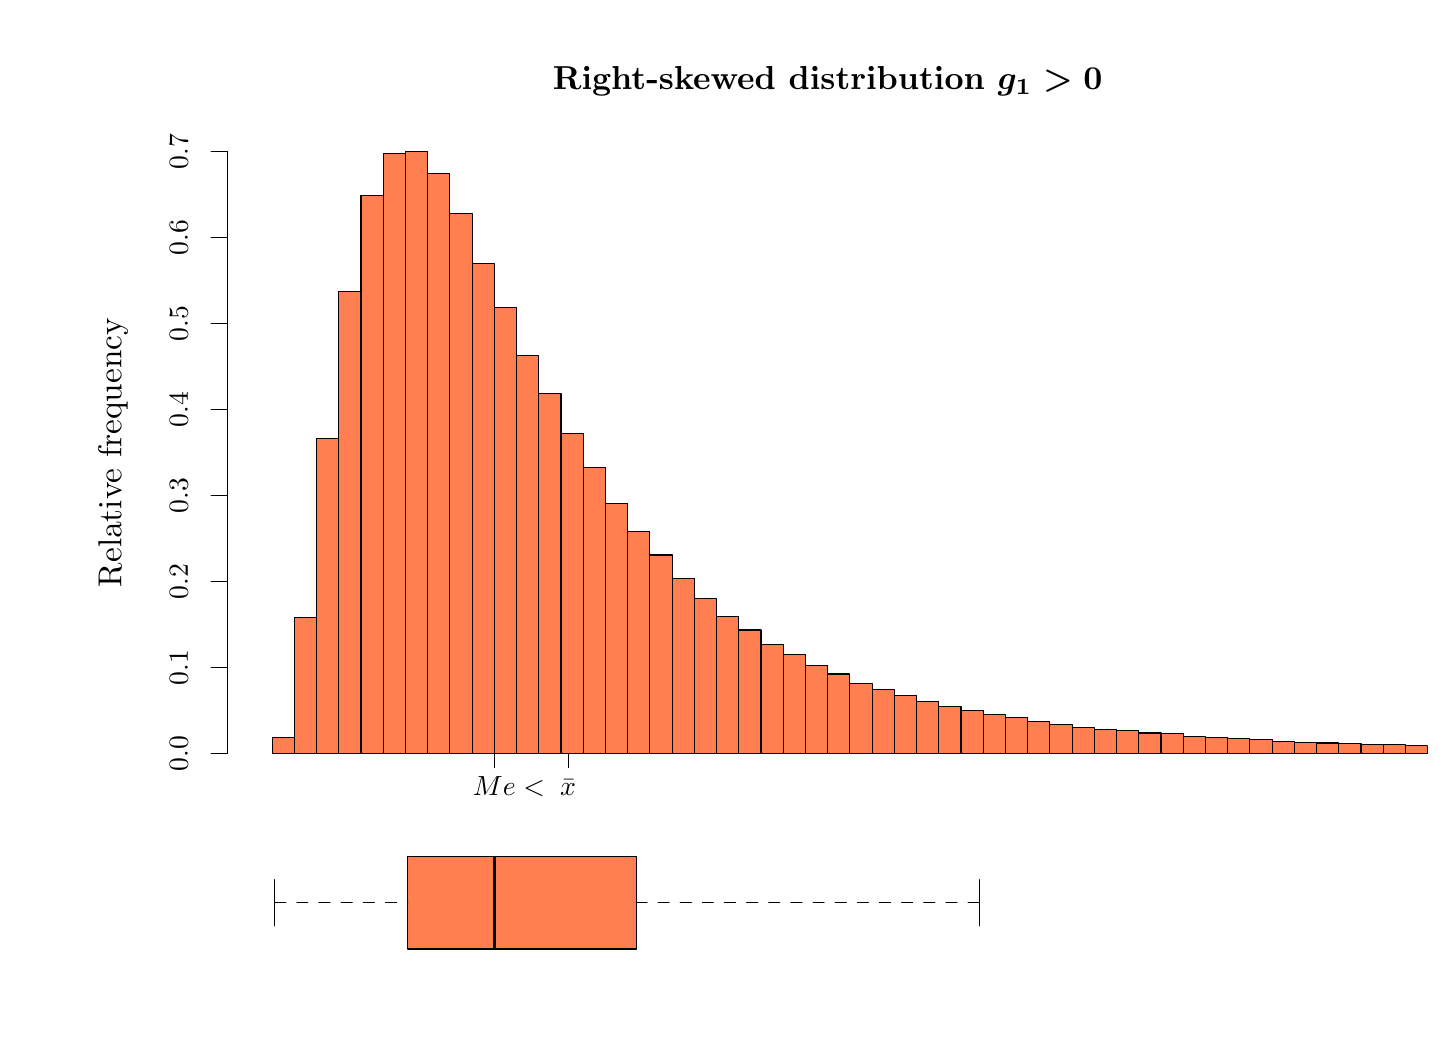
\begin{tikzpicture}[x=1pt,y=1pt]
\definecolor{fillColor}{RGB}{255,255,255}
\path[use as bounding box,fill=fillColor,fill opacity=0.00] (0,0) rectangle (505.89,361.35);
\begin{scope}
\path[clip] (  0.00, 90.34) rectangle (505.89,361.35);
\definecolor{drawColor}{RGB}{0,0,0}

\node[text=drawColor,anchor=base,inner sep=0pt, outer sep=0pt, scale=  1.20, font=\boldmath] at (289.08,339.14)
{\bfseries Right-skewed distribution $g_1>0$};

\node[text=drawColor,anchor=base,inner sep=0pt, outer sep=0pt, scale=  1.20] at (289.08, 44.74) {x};

\node[text=drawColor,rotate= 90.00,anchor=base,inner sep=0pt, outer sep=0pt, scale=  1.20] at ( 33.87,207.78) {Relative frequency};
\end{scope}
\begin{scope}
\path[clip] (  0.00,  0.00) rectangle (505.89,361.35);
\definecolor{drawColor}{RGB}{0,0,0}

\path[draw=drawColor,line width= 0.4pt,line join=round,line cap=round] ( 72.27, 99.04) -- ( 72.27,316.56);

\path[draw=drawColor,line width= 0.4pt,line join=round,line cap=round] ( 72.27, 99.04) -- ( 66.27, 99.04);

\path[draw=drawColor,line width= 0.4pt,line join=round,line cap=round] ( 72.27,130.11) -- ( 66.27,130.11);

\path[draw=drawColor,line width= 0.4pt,line join=round,line cap=round] ( 72.27,161.19) -- ( 66.27,161.19);

\path[draw=drawColor,line width= 0.4pt,line join=round,line cap=round] ( 72.27,192.26) -- ( 66.27,192.26);

\path[draw=drawColor,line width= 0.4pt,line join=round,line cap=round] ( 72.27,223.33) -- ( 66.27,223.33);

\path[draw=drawColor,line width= 0.4pt,line join=round,line cap=round] ( 72.27,254.41) -- ( 66.27,254.41);

\path[draw=drawColor,line width= 0.4pt,line join=round,line cap=round] ( 72.27,285.48) -- ( 66.27,285.48);

\path[draw=drawColor,line width= 0.4pt,line join=round,line cap=round] ( 72.27,316.56) -- ( 66.27,316.56);

\node[text=drawColor,rotate= 90.00,anchor=base,inner sep=0pt, outer sep=0pt, scale=  1.00] at ( 57.87, 99.04) {0.0};

\node[text=drawColor,rotate= 90.00,anchor=base,inner sep=0pt, outer sep=0pt, scale=  1.00] at ( 57.87,130.11) {0.1};

\node[text=drawColor,rotate= 90.00,anchor=base,inner sep=0pt, outer sep=0pt, scale=  1.00] at ( 57.87,161.19) {0.2};

\node[text=drawColor,rotate= 90.00,anchor=base,inner sep=0pt, outer sep=0pt, scale=  1.00] at ( 57.87,192.26) {0.3};

\node[text=drawColor,rotate= 90.00,anchor=base,inner sep=0pt, outer sep=0pt, scale=  1.00] at ( 57.87,223.33) {0.4};

\node[text=drawColor,rotate= 90.00,anchor=base,inner sep=0pt, outer sep=0pt, scale=  1.00] at ( 57.87,254.41) {0.5};

\node[text=drawColor,rotate= 90.00,anchor=base,inner sep=0pt, outer sep=0pt, scale=  1.00] at ( 57.87,285.48) {0.6};

\node[text=drawColor,rotate= 90.00,anchor=base,inner sep=0pt, outer sep=0pt, scale=  1.00] at ( 57.87,316.56) {0.7};
\end{scope}
\begin{scope}
\path[clip] ( 72.27, 90.34) rectangle (505.89,325.21);
\definecolor{drawColor}{RGB}{0,0,0}
\definecolor{fillColor}{RGB}{255,127,80}

\path[draw=drawColor,line width= 0.4pt,line join=round,line cap=round,fill=fillColor] ( 88.33, 99.04) rectangle ( 96.36,104.80);

\path[draw=drawColor,line width= 0.4pt,line join=round,line cap=round,fill=fillColor] ( 96.36, 99.04) rectangle (104.39,148.07);

\path[draw=drawColor,line width= 0.4pt,line join=round,line cap=round,fill=fillColor] (104.39, 99.04) rectangle (112.42,212.96);

\path[draw=drawColor,line width= 0.4pt,line join=round,line cap=round,fill=fillColor] (112.42, 99.04) rectangle (120.45,266.13);

\path[draw=drawColor,line width= 0.4pt,line join=round,line cap=round,fill=fillColor] (120.45, 99.04) rectangle (128.48,300.70);

\path[draw=drawColor,line width= 0.4pt,line join=round,line cap=round,fill=fillColor] (128.48, 99.04) rectangle (136.51,316.02);

\path[draw=drawColor,line width= 0.4pt,line join=round,line cap=round,fill=fillColor] (136.51, 99.04) rectangle (144.54,316.52);

\path[draw=drawColor,line width= 0.4pt,line join=round,line cap=round,fill=fillColor] (144.54, 99.04) rectangle (152.57,308.80);

\path[draw=drawColor,line width= 0.4pt,line join=round,line cap=round,fill=fillColor] (152.57, 99.04) rectangle (160.60,294.26);

\path[draw=drawColor,line width= 0.4pt,line join=round,line cap=round,fill=fillColor] (160.60, 99.04) rectangle (168.63,276.22);

\path[draw=drawColor,line width= 0.4pt,line join=round,line cap=round,fill=fillColor] (168.63, 99.04) rectangle (176.66,260.10);

\path[draw=drawColor,line width= 0.4pt,line join=round,line cap=round,fill=fillColor] (176.66, 99.04) rectangle (184.69,243.00);

\path[draw=drawColor,line width= 0.4pt,line join=round,line cap=round,fill=fillColor] (184.69, 99.04) rectangle (192.72,229.05);

\path[draw=drawColor,line width= 0.4pt,line join=round,line cap=round,fill=fillColor] (192.72, 99.04) rectangle (200.75,214.68);

\path[draw=drawColor,line width= 0.4pt,line join=round,line cap=round,fill=fillColor] (200.75, 99.04) rectangle (208.78,202.38);

\path[draw=drawColor,line width= 0.4pt,line join=round,line cap=round,fill=fillColor] (208.78, 99.04) rectangle (216.81,189.41);

\path[draw=drawColor,line width= 0.4pt,line join=round,line cap=round,fill=fillColor] (216.81, 99.04) rectangle (224.84,179.32);

\path[draw=drawColor,line width= 0.4pt,line join=round,line cap=round,fill=fillColor] (224.84, 99.04) rectangle (232.87,170.80);

\path[draw=drawColor,line width= 0.4pt,line join=round,line cap=round,fill=fillColor] (232.87, 99.04) rectangle (240.90,162.23);

\path[draw=drawColor,line width= 0.4pt,line join=round,line cap=round,fill=fillColor] (240.90, 99.04) rectangle (248.93,154.93);

\path[draw=drawColor,line width= 0.4pt,line join=round,line cap=round,fill=fillColor] (248.93, 99.04) rectangle (256.96,148.65);

\path[draw=drawColor,line width= 0.4pt,line join=round,line cap=round,fill=fillColor] (256.96, 99.04) rectangle (264.99,143.69);

\path[draw=drawColor,line width= 0.4pt,line join=round,line cap=round,fill=fillColor] (264.99, 99.04) rectangle (273.02,138.53);

\path[draw=drawColor,line width= 0.4pt,line join=round,line cap=round,fill=fillColor] (273.02, 99.04) rectangle (281.05,134.88);

\path[draw=drawColor,line width= 0.4pt,line join=round,line cap=round,fill=fillColor] (281.05, 99.04) rectangle (289.08,131.01);

\path[draw=drawColor,line width= 0.4pt,line join=round,line cap=round,fill=fillColor] (289.08, 99.04) rectangle (297.11,127.81);

\path[draw=drawColor,line width= 0.4pt,line join=round,line cap=round,fill=fillColor] (297.11, 99.04) rectangle (305.14,124.52);

\path[draw=drawColor,line width= 0.4pt,line join=round,line cap=round,fill=fillColor] (305.14, 99.04) rectangle (313.17,122.32);

\path[draw=drawColor,line width= 0.4pt,line join=round,line cap=round,fill=fillColor] (313.17, 99.04) rectangle (321.20,120.15);

\path[draw=drawColor,line width= 0.4pt,line join=round,line cap=round,fill=fillColor] (321.20, 99.04) rectangle (329.23,117.91);

\path[draw=drawColor,line width= 0.4pt,line join=round,line cap=round,fill=fillColor] (329.23, 99.04) rectangle (337.26,115.92);

\path[draw=drawColor,line width= 0.4pt,line join=round,line cap=round,fill=fillColor] (337.26, 99.04) rectangle (345.29,114.52);

\path[draw=drawColor,line width= 0.4pt,line join=round,line cap=round,fill=fillColor] (345.29, 99.04) rectangle (353.32,113.03);

\path[draw=drawColor,line width= 0.4pt,line join=round,line cap=round,fill=fillColor] (353.32, 99.04) rectangle (361.35,112.08);

\path[draw=drawColor,line width= 0.4pt,line join=round,line cap=round,fill=fillColor] (361.35, 99.04) rectangle (369.38,110.55);

\path[draw=drawColor,line width= 0.4pt,line join=round,line cap=round,fill=fillColor] (369.38, 99.04) rectangle (377.41,109.66);

\path[draw=drawColor,line width= 0.4pt,line join=round,line cap=round,fill=fillColor] (377.41, 99.04) rectangle (385.44,108.62);

\path[draw=drawColor,line width= 0.4pt,line join=round,line cap=round,fill=fillColor] (385.44, 99.04) rectangle (393.47,107.87);

\path[draw=drawColor,line width= 0.4pt,line join=round,line cap=round,fill=fillColor] (393.47, 99.04) rectangle (401.50,107.43);

\path[draw=drawColor,line width= 0.4pt,line join=round,line cap=round,fill=fillColor] (401.50, 99.04) rectangle (409.53,106.46);

\path[draw=drawColor,line width= 0.4pt,line join=round,line cap=round,fill=fillColor] (409.53, 99.04) rectangle (417.56,106.17);

\path[draw=drawColor,line width= 0.4pt,line join=round,line cap=round,fill=fillColor] (417.56, 99.04) rectangle (425.59,105.22);

\path[draw=drawColor,line width= 0.4pt,line join=round,line cap=round,fill=fillColor] (425.59, 99.04) rectangle (433.62,104.90);

\path[draw=drawColor,line width= 0.4pt,line join=round,line cap=round,fill=fillColor] (433.62, 99.04) rectangle (441.65,104.45);

\path[draw=drawColor,line width= 0.4pt,line join=round,line cap=round,fill=fillColor] (441.65, 99.04) rectangle (449.68,104.07);

\path[draw=drawColor,line width= 0.4pt,line join=round,line cap=round,fill=fillColor] (449.68, 99.04) rectangle (457.71,103.49);

\path[draw=drawColor,line width= 0.4pt,line join=round,line cap=round,fill=fillColor] (457.71, 99.04) rectangle (465.74,103.20);

\path[draw=drawColor,line width= 0.4pt,line join=round,line cap=round,fill=fillColor] (465.74, 99.04) rectangle (473.77,102.87);

\path[draw=drawColor,line width= 0.4pt,line join=round,line cap=round,fill=fillColor] (473.77, 99.04) rectangle (481.80,102.72);

\path[draw=drawColor,line width= 0.4pt,line join=round,line cap=round,fill=fillColor] (481.80, 99.04) rectangle (489.83,102.30);

\path[draw=drawColor,line width= 0.4pt,line join=round,line cap=round,fill=fillColor] (489.83, 99.04) rectangle (497.86,102.22);

\path[draw=drawColor,line width= 0.4pt,line join=round,line cap=round,fill=fillColor] (497.86, 99.04) rectangle (505.89,101.90);

\path[draw=drawColor,line width= 0.4pt,line join=round,line cap=round,fill=fillColor] (505.89, 99.04) rectangle (513.92,101.70);
\end{scope}
\begin{scope}
\path[clip] (  0.00,  0.00) rectangle (505.89,361.35);
\definecolor{drawColor}{RGB}{0,0,0}
\path[draw=drawColor,line width= 0.4pt,line join=round,line cap=round] (168.61, 99.04) -- (168.61, 94);
\path[draw=drawColor,line width= 0.4pt,line join=round,line cap=round] (195.28, 99.04) -- (195.28, 94);
\node[text=drawColor,anchor=base,inner sep=0pt, outer sep=0pt, scale=  1.00] at (168.61, 84) {$Me$};
\node[text=drawColor,anchor=base,inner sep=0pt, outer sep=0pt, scale=  1.00] at (183, 84) {$<$};
\node[text=drawColor,anchor=base,inner sep=0pt, outer sep=0pt, scale=  1.00] at (195.28, 84) {$\bar x$};
\end{scope}
\begin{scope}
\path[clip] ( 72.27,  0.00) rectangle (505.89, 90.34);
\definecolor{fillColor}{RGB}{255,127,80}

\path[fill=fillColor] (137.34, 28.44) --
	(137.34, 61.90) --
	(219.92, 61.90) --
	(219.92, 28.44) --
	cycle;
\definecolor{drawColor}{RGB}{0,0,0}

\path[draw=drawColor,line width= 1.2pt,line join=round] (168.61, 28.44) -- (168.61, 61.90);

\path[draw=drawColor,line width= 0.4pt,dash pattern=on 4pt off 4pt ,line join=round,line cap=round] ( 89.27, 45.17) -- (137.34, 45.17);

\path[draw=drawColor,line width= 0.4pt,dash pattern=on 4pt off 4pt ,line join=round,line cap=round] (343.80, 45.17) -- (219.92, 45.17);

\path[draw=drawColor,line width= 0.4pt,line join=round,line cap=round] ( 89.27, 36.80) -- ( 89.27, 53.53);

\path[draw=drawColor,line width= 0.4pt,line join=round,line cap=round] (343.80, 36.80) -- (343.80, 53.53);

\path[draw=drawColor,line width= 0.4pt,line join=round,line cap=round] (137.34, 28.44) --
	(137.34, 61.90) --
	(219.92, 61.90) --
	(219.92, 28.44) --
	(137.34, 28.44);
\end{scope}
\end{tikzpicture}
}
\end{center}
\end{frame}


%---------------------------------------------------------------------slide----
\begin{frame}
\frametitle{Coefficient of skewness calculation}
\framesubtitle{Example with grouped data}
Using the frequency table of the sample with the heights of students and adding a new column with the deviations to
the mean $\bar x = 174.67$ cm to cube, we get
\[
\setlength\arraycolsep{3mm}
\setlength\arrayrulewidth{0.5pt}
\begin{array}{rrrrr}
\hline
\multicolumn{1}{c}{X} & \multicolumn{1}{c}{x_i} & \multicolumn{1}{c}{n_i} & \multicolumn{1}{c}{x_i-\bar x} & \multicolumn{1}{c}{(x_i-\bar x)^3 n_i} \\
\hline
(150,160] & 155 & 2 & -19.67 & -15221.00\\
(160,170] & 165 & 8 & -9.67 & -7233.85\\
(170,180] & 175 & 11 & 0.33 & 0.40\\
(180,190] & 185 & 7 & 10.33 & 7716.12\\
(190,200] & 195 & 2 & 20.33 & 16805.14\\
\hline
\sum &  & 30 & & 2066.81 \\
\hline
\end{array}
\]
\[
g_1 = \frac{\sum (x_i-\bar x)^3n_i/n}{s^3} = \frac{2066.81/30}{10.1^3} = 0.07.
\]
As it is close to 0, that means that the distribution of heights is fairly symmetrical. 
\end{frame}


%---------------------------------------------------------------------slide----
\begin{frame}
\frametitle{Coefficient of kurtosis}
\begin{definition}[Sample coefficient of kurtosis $g_2$]
The \emph{sample coefficient of kurtosis} of a variable $X$ is the average of the deviations of values from the sample
mean to the fourth power, divided by the standard deviation to the fourth power and minus 3. 
\[g_2 = \frac{\sum (x_i-\bar x)^4 n_i/n}{s^4}-3 = \frac{\sum (x_i-\bar x)^4 f_i}{s^4}-3\]
\end{definition}

The coefficient of kurtosis measures the the length of tails or the peakness of distribution with respect to normal
(bell-shaped) distribution of reference.
\begin{itemize}
\item $g_2=0$ indicates that the distribution has the same tails and peakedness than a normal distribution
(\emph{mesokurtic}).
\item $g_2<0$ indicates that the distribution has longer tails and lower peakedness than a normal distribution
(\emph{platykurtic}).
\item $g_2>0$ indicates that the distribution has shorter tails and higher peakedness than a normal distribution 
(\emph{leptokurtic}).
\end{itemize}
\end{frame}


%---------------------------------------------------------------------slide----
\begin{frame}
\frametitle{Coefficient of kurtosis}
\framesubtitle{Example of mesokurtic distribution}
\begin{center}
\tikzsetnextfilename{descriptive/mesokurtic_distribution}
\scalebox{0.6}{% Created by tikzDevice version 0.8.1 on 2015-11-20 15:35:03
% !TEX encoding = UTF-8 Unicode
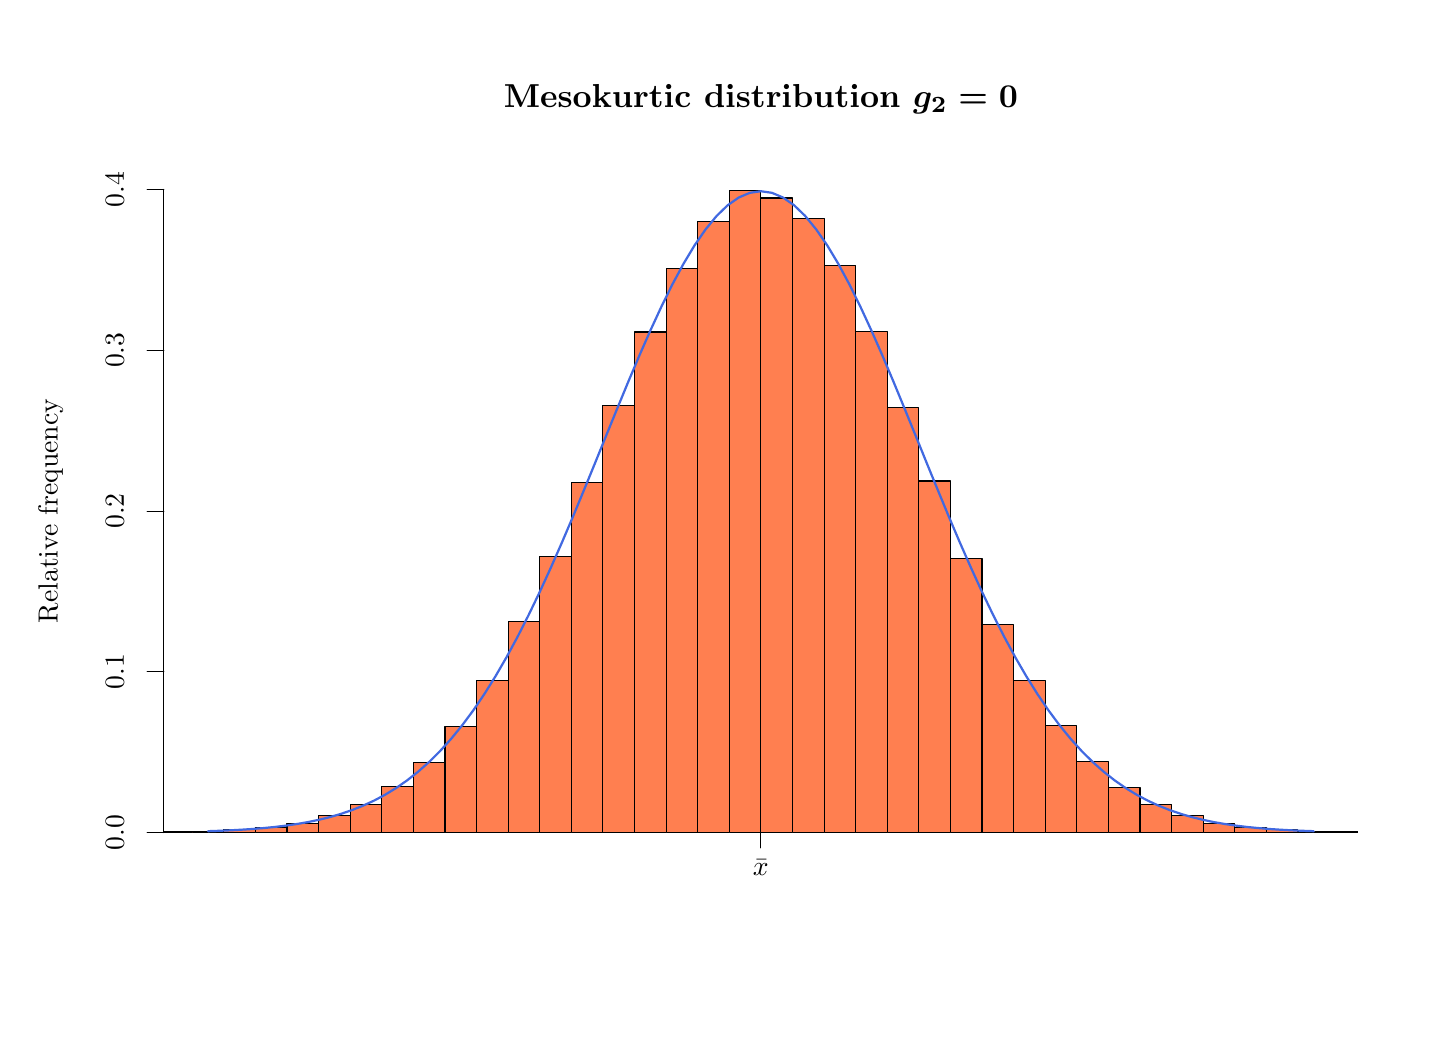
\begin{tikzpicture}[x=1pt,y=1pt]
\definecolor{fillColor}{RGB}{255,255,255}
\path[use as bounding box,fill=fillColor,fill opacity=0.00] (0,0) rectangle (505.89,361.35);
\begin{scope}
\path[clip] (  0.00,  0.00) rectangle (505.89,361.35);
\definecolor{drawColor}{RGB}{0,0,0}

\node[text=drawColor,anchor=base,inner sep=0pt, outer sep=0pt, scale=  1.20, font=\boldmath] at (264.94,332.61)
{\bfseries Mesokurtic distribution $g_2=0$};

\node[text=drawColor,rotate= 90.00,anchor=base,inner sep=0pt, outer sep=0pt, scale=  1.00] at ( 10.80,186.67) {Relative frequency};
\end{scope}
\begin{scope}
\path[clip] ( 49.20, 61.20) rectangle (480.69,312.15);
\definecolor{drawColor}{RGB}{0,0,0}
\definecolor{fillColor}{RGB}{255,127,80}

\path[draw=drawColor,line width= 0.4pt,line join=round,line cap=round,fill=fillColor] ( -9.02, 70.49) rectangle (  2.40, 70.50);

\path[draw=drawColor,line width= 0.4pt,line join=round,line cap=round,fill=fillColor] (  2.40, 70.49) rectangle ( 13.81, 70.50);

\path[draw=drawColor,line width= 0.4pt,line join=round,line cap=round,fill=fillColor] ( 13.81, 70.49) rectangle ( 25.23, 70.51);

\path[draw=drawColor,line width= 0.4pt,line join=round,line cap=round,fill=fillColor] ( 25.23, 70.49) rectangle ( 36.64, 70.54);

\path[draw=drawColor,line width= 0.4pt,line join=round,line cap=round,fill=fillColor] ( 36.64, 70.49) rectangle ( 48.06, 70.59);

\path[draw=drawColor,line width= 0.4pt,line join=round,line cap=round,fill=fillColor] ( 48.06, 70.49) rectangle ( 59.47, 70.76);

\path[draw=drawColor,line width= 0.4pt,line join=round,line cap=round,fill=fillColor] ( 59.47, 70.49) rectangle ( 70.89, 71.04);

\path[draw=drawColor,line width= 0.4pt,line join=round,line cap=round,fill=fillColor] ( 70.89, 70.49) rectangle ( 82.30, 71.48);

\path[draw=drawColor,line width= 0.4pt,line join=round,line cap=round,fill=fillColor] ( 82.30, 70.49) rectangle ( 93.72, 72.39);

\path[draw=drawColor,line width= 0.4pt,line join=round,line cap=round,fill=fillColor] ( 93.72, 70.49) rectangle (105.13, 73.87);

\path[draw=drawColor,line width= 0.4pt,line join=round,line cap=round,fill=fillColor] (105.13, 70.49) rectangle (116.55, 76.63);

\path[draw=drawColor,line width= 0.4pt,line join=round,line cap=round,fill=fillColor] (116.55, 70.49) rectangle (127.96, 80.62);

\path[draw=drawColor,line width= 0.4pt,line join=round,line cap=round,fill=fillColor] (127.96, 70.49) rectangle (139.38, 87.11);

\path[draw=drawColor,line width= 0.4pt,line join=round,line cap=round,fill=fillColor] (139.38, 70.49) rectangle (150.79, 95.88);

\path[draw=drawColor,line width= 0.4pt,line join=round,line cap=round,fill=fillColor] (150.79, 70.49) rectangle (162.21,108.91);

\path[draw=drawColor,line width= 0.4pt,line join=round,line cap=round,fill=fillColor] (162.21, 70.49) rectangle (173.62,125.60);

\path[draw=drawColor,line width= 0.4pt,line join=round,line cap=round,fill=fillColor] (173.62, 70.49) rectangle (185.04,146.75);

\path[draw=drawColor,line width= 0.4pt,line join=round,line cap=round,fill=fillColor] (185.04, 70.49) rectangle (196.45,170.20);

\path[draw=drawColor,line width= 0.4pt,line join=round,line cap=round,fill=fillColor] (196.45, 70.49) rectangle (207.87,197.01);

\path[draw=drawColor,line width= 0.4pt,line join=round,line cap=round,fill=fillColor] (207.87, 70.49) rectangle (219.28,224.77);

\path[draw=drawColor,line width= 0.4pt,line join=round,line cap=round,fill=fillColor] (219.28, 70.49) rectangle (230.70,251.37);

\path[draw=drawColor,line width= 0.4pt,line join=round,line cap=round,fill=fillColor] (230.70, 70.49) rectangle (242.11,274.44);

\path[draw=drawColor,line width= 0.4pt,line join=round,line cap=round,fill=fillColor] (242.11, 70.49) rectangle (253.53,291.16);

\path[draw=drawColor,line width= 0.4pt,line join=round,line cap=round,fill=fillColor] (253.53, 70.49) rectangle (264.94,302.52);

\path[draw=drawColor,line width= 0.4pt,line join=round,line cap=round,fill=fillColor] (264.94, 70.49) rectangle (276.36,299.78);

\path[draw=drawColor,line width= 0.4pt,line join=round,line cap=round,fill=fillColor] (276.36, 70.49) rectangle (287.78,292.37);

\path[draw=drawColor,line width= 0.4pt,line join=round,line cap=round,fill=fillColor] (287.78, 70.49) rectangle (299.19,275.50);

\path[draw=drawColor,line width= 0.4pt,line join=round,line cap=round,fill=fillColor] (299.19, 70.49) rectangle (310.61,251.48);

\path[draw=drawColor,line width= 0.4pt,line join=round,line cap=round,fill=fillColor] (310.61, 70.49) rectangle (322.02,224.09);

\path[draw=drawColor,line width= 0.4pt,line join=round,line cap=round,fill=fillColor] (322.02, 70.49) rectangle (333.44,197.54);

\path[draw=drawColor,line width= 0.4pt,line join=round,line cap=round,fill=fillColor] (333.44, 70.49) rectangle (344.85,169.59);

\path[draw=drawColor,line width= 0.4pt,line join=round,line cap=round,fill=fillColor] (344.85, 70.49) rectangle (356.27,145.54);

\path[draw=drawColor,line width= 0.4pt,line join=round,line cap=round,fill=fillColor] (356.27, 70.49) rectangle (367.68,125.35);

\path[draw=drawColor,line width= 0.4pt,line join=round,line cap=round,fill=fillColor] (367.68, 70.49) rectangle (379.10,109.13);

\path[draw=drawColor,line width= 0.4pt,line join=round,line cap=round,fill=fillColor] (379.10, 70.49) rectangle (390.51, 96.33);

\path[draw=drawColor,line width= 0.4pt,line join=round,line cap=round,fill=fillColor] (390.51, 70.49) rectangle (401.93, 86.82);

\path[draw=drawColor,line width= 0.4pt,line join=round,line cap=round,fill=fillColor] (401.93, 70.49) rectangle (413.34, 80.76);

\path[draw=drawColor,line width= 0.4pt,line join=round,line cap=round,fill=fillColor] (413.34, 70.49) rectangle (424.76, 76.70);

\path[draw=drawColor,line width= 0.4pt,line join=round,line cap=round,fill=fillColor] (424.76, 70.49) rectangle (436.17, 73.85);

\path[draw=drawColor,line width= 0.4pt,line join=round,line cap=round,fill=fillColor] (436.17, 70.49) rectangle (447.59, 72.34);

\path[draw=drawColor,line width= 0.4pt,line join=round,line cap=round,fill=fillColor] (447.59, 70.49) rectangle (459.00, 71.51);

\path[draw=drawColor,line width= 0.4pt,line join=round,line cap=round,fill=fillColor] (459.00, 70.49) rectangle (470.42, 70.99);

\path[draw=drawColor,line width= 0.4pt,line join=round,line cap=round,fill=fillColor] (470.42, 70.49) rectangle (481.83, 70.76);

\path[draw=drawColor,line width= 0.4pt,line join=round,line cap=round,fill=fillColor] (481.83, 70.49) rectangle (493.25, 70.62);

\path[draw=drawColor,line width= 0.4pt,line join=round,line cap=round,fill=fillColor] (493.25, 70.49) rectangle (504.66, 70.53);

\path[draw=drawColor,line width= 0.4pt,line join=round,line cap=round,fill=fillColor] (504.66, 70.49) rectangle (516.08, 70.52);
\end{scope}
\begin{scope}
\path[clip] (  0.00,  0.00) rectangle (505.89,361.35);
\definecolor{drawColor}{RGB}{0,0,0}

\path[draw=drawColor,line width= 0.4pt,line join=round,line cap=round] (264.92, 70.49) -- (264.92, 65);

\node[text=drawColor,anchor=base,inner sep=0pt, outer sep=0pt, scale=  1.00] at (264.92, 55) {$\bar x$};

\path[draw=drawColor,line width= 0.4pt,line join=round,line cap=round] ( 49.20, 70.49) -- ( 49.20,302.86);

\path[draw=drawColor,line width= 0.4pt,line join=round,line cap=round] ( 49.20, 70.49) -- ( 43.20, 70.49);

\path[draw=drawColor,line width= 0.4pt,line join=round,line cap=round] ( 49.20,128.58) -- ( 43.20,128.58);

\path[draw=drawColor,line width= 0.4pt,line join=round,line cap=round] ( 49.20,186.67) -- ( 43.20,186.67);

\path[draw=drawColor,line width= 0.4pt,line join=round,line cap=round] ( 49.20,244.77) -- ( 43.20,244.77);

\path[draw=drawColor,line width= 0.4pt,line join=round,line cap=round] ( 49.20,302.86) -- ( 43.20,302.86);

\node[text=drawColor,rotate= 90.00,anchor=base,inner sep=0pt, outer sep=0pt, scale=  1.00] at ( 34.80, 70.49) {0.0};

\node[text=drawColor,rotate= 90.00,anchor=base,inner sep=0pt, outer sep=0pt, scale=  1.00] at ( 34.80,128.58) {0.1};

\node[text=drawColor,rotate= 90.00,anchor=base,inner sep=0pt, outer sep=0pt, scale=  1.00] at ( 34.80,186.67) {0.2};

\node[text=drawColor,rotate= 90.00,anchor=base,inner sep=0pt, outer sep=0pt, scale=  1.00] at ( 34.80,244.77) {0.3};

\node[text=drawColor,rotate= 90.00,anchor=base,inner sep=0pt, outer sep=0pt, scale=  1.00] at ( 34.80,302.86) {0.4};
\end{scope}
\begin{scope}
\path[clip] ( 49.20, 61.20) rectangle (480.69,312.15);
\definecolor{drawColor}{RGB}{65,105,225}

\path[draw=drawColor,line width= 0.8pt,line join=round,line cap=round] ( 65.18, 71.00) --
	( 69.18, 71.14) --
	( 73.17, 71.31) --
	( 77.17, 71.53) --
	( 81.16, 71.79) --
	( 85.16, 72.12) --
	( 89.15, 72.51) --
	( 93.15, 72.99) --
	( 97.14, 73.57) --
	(101.14, 74.26) --
	(105.13, 75.09) --
	(109.13, 76.07) --
	(113.12, 77.23) --
	(117.12, 78.59) --
	(121.11, 80.18) --
	(125.11, 82.02) --
	(129.11, 84.14) --
	(133.10, 86.57) --
	(137.10, 89.35) --
	(141.09, 92.50) --
	(145.09, 96.04) --
	(149.08,100.02) --
	(153.08,104.44) --
	(157.07,109.34) --
	(161.07,114.73) --
	(165.06,120.61) --
	(169.06,127.01) --
	(173.05,133.90) --
	(177.05,141.29) --
	(181.04,149.16) --
	(185.04,157.47) --
	(189.03,166.19) --
	(193.03,175.27) --
	(197.03,184.65) --
	(201.02,194.27) --
	(205.02,204.03) --
	(209.01,213.87) --
	(213.01,223.67) --
	(217.00,233.35) --
	(221.00,242.79) --
	(224.99,251.88) --
	(228.99,260.53) --
	(232.98,268.61) --
	(236.98,276.03) --
	(240.97,282.68) --
	(244.97,288.47) --
	(248.96,293.33) --
	(252.96,297.19) --
	(256.95,299.98) --
	(260.95,301.67) --
	(264.94,302.24) --
	(268.94,301.67) --
	(272.94,299.98) --
	(276.93,297.19) --
	(280.93,293.33) --
	(284.92,288.47) --
	(288.92,282.68) --
	(292.91,276.03) --
	(296.91,268.61) --
	(300.90,260.53) --
	(304.90,251.88) --
	(308.89,242.79) --
	(312.89,233.35) --
	(316.88,223.67) --
	(320.88,213.87) --
	(324.87,204.03) --
	(328.87,194.27) --
	(332.86,184.65) --
	(336.86,175.27) --
	(340.86,166.19) --
	(344.85,157.47) --
	(348.85,149.16) --
	(352.84,141.29) --
	(356.84,133.90) --
	(360.83,127.01) --
	(364.83,120.61) --
	(368.82,114.73) --
	(372.82,109.34) --
	(376.81,104.44) --
	(380.81,100.02) --
	(384.80, 96.04) --
	(388.80, 92.50) --
	(392.79, 89.35) --
	(396.79, 86.57) --
	(400.78, 84.14) --
	(404.78, 82.02) --
	(408.77, 80.18) --
	(412.77, 78.59) --
	(416.77, 77.23) --
	(420.76, 76.07) --
	(424.76, 75.09) --
	(428.75, 74.26) --
	(432.75, 73.57) --
	(436.74, 72.99) --
	(440.74, 72.51) --
	(444.73, 72.12) --
	(448.73, 71.79) --
	(452.72, 71.53) --
	(456.72, 71.31) --
	(460.71, 71.14) --
	(464.71, 71.00);
\end{scope}
\end{tikzpicture}
}
\end{center}
\end{frame}


%---------------------------------------------------------------------slide----
\begin{frame}
\frametitle{Coefficient of kurtosis}
\framesubtitle{Example of platykurtic distribution}
\begin{center}
\tikzsetnextfilename{descriptive/platykurtic_distribution}
\scalebox{0.6}{% Created by tikzDevice version 0.8.1 on 2015-11-21 14:38:50
% !TEX encoding = UTF-8 Unicode
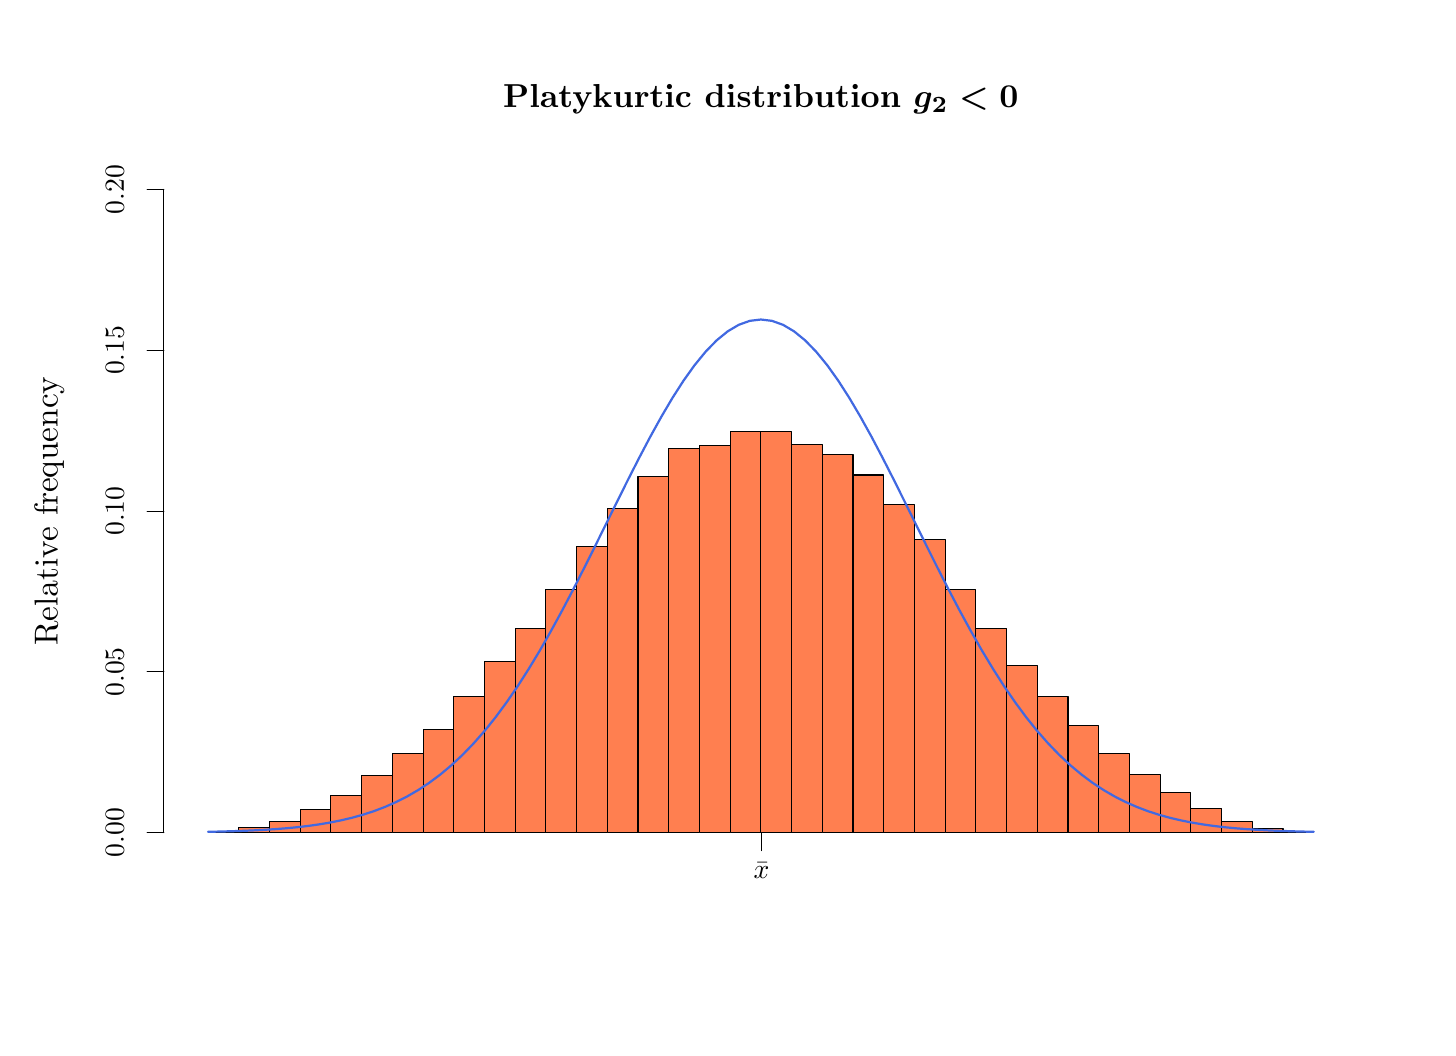
\begin{tikzpicture}[x=1pt,y=1pt]
\definecolor{fillColor}{RGB}{255,255,255}
\path[use as bounding box,fill=fillColor,fill opacity=0.00] (0,0) rectangle (505.89,361.35);
\begin{scope}
\path[clip] (  0.00,  0.00) rectangle (505.89,361.35);
\definecolor{drawColor}{RGB}{0,0,0}

\node[text=drawColor,anchor=base,inner sep=0pt, outer sep=0pt, scale=  1.20, font=\boldmath] at (264.94,332.61)
{\bfseries Platykurtic distribution $g_2<0$};

\node[text=drawColor,rotate= 90.00,anchor=base,inner sep=0pt, outer sep=0pt, scale=  1.20] at ( 10.80,186.67)
{Relative frequency};
\end{scope}
\begin{scope}
\path[clip] ( 49.20, 61.20) rectangle (480.69,312.15);
\definecolor{drawColor}{RGB}{0,0,0}
\definecolor{fillColor}{RGB}{255,127,80}

\path[draw=drawColor,line width= 0.4pt,line join=round,line cap=round,fill=fillColor] ( 65.18, 70.49) rectangle ( 76.28, 70.66);

\path[draw=drawColor,line width= 0.4pt,line join=round,line cap=round,fill=fillColor] ( 76.28, 70.49) rectangle ( 87.38, 72.27);

\path[draw=drawColor,line width= 0.4pt,line join=round,line cap=round,fill=fillColor] ( 87.38, 70.49) rectangle ( 98.48, 74.36);

\path[draw=drawColor,line width= 0.4pt,line join=round,line cap=round,fill=fillColor] ( 98.48, 70.49) rectangle (109.57, 78.85);

\path[draw=drawColor,line width= 0.4pt,line join=round,line cap=round,fill=fillColor] (109.57, 70.49) rectangle (120.67, 84.04);

\path[draw=drawColor,line width= 0.4pt,line join=round,line cap=round,fill=fillColor] (120.67, 70.49) rectangle (131.77, 91.10);

\path[draw=drawColor,line width= 0.4pt,line join=round,line cap=round,fill=fillColor] (131.77, 70.49) rectangle (142.87, 98.97);

\path[draw=drawColor,line width= 0.4pt,line join=round,line cap=round,fill=fillColor] (142.87, 70.49) rectangle (153.97,107.87);

\path[draw=drawColor,line width= 0.4pt,line join=round,line cap=round,fill=fillColor] (153.97, 70.49) rectangle (165.06,119.51);

\path[draw=drawColor,line width= 0.4pt,line join=round,line cap=round,fill=fillColor] (165.06, 70.49) rectangle (176.16,132.20);

\path[draw=drawColor,line width= 0.4pt,line join=round,line cap=round,fill=fillColor] (176.16, 70.49) rectangle (187.26,144.35);

\path[draw=drawColor,line width= 0.4pt,line join=round,line cap=round,fill=fillColor] (187.26, 70.49) rectangle (198.36,158.29);

\path[draw=drawColor,line width= 0.4pt,line join=round,line cap=round,fill=fillColor] (198.36, 70.49) rectangle (209.46,173.78);

\path[draw=drawColor,line width= 0.4pt,line join=round,line cap=round,fill=fillColor] (209.46, 70.49) rectangle (220.55,187.44);

\path[draw=drawColor,line width= 0.4pt,line join=round,line cap=round,fill=fillColor] (220.55, 70.49) rectangle (231.65,199.20);

\path[draw=drawColor,line width= 0.4pt,line join=round,line cap=round,fill=fillColor] (231.65, 70.49) rectangle (242.75,209.17);

\path[draw=drawColor,line width= 0.4pt,line join=round,line cap=round,fill=fillColor] (242.75, 70.49) rectangle (253.85,210.52);

\path[draw=drawColor,line width= 0.4pt,line join=round,line cap=round,fill=fillColor] (253.85, 70.49) rectangle (264.94,215.44);

\path[draw=drawColor,line width= 0.4pt,line join=round,line cap=round,fill=fillColor] (264.94, 70.49) rectangle (276.04,215.27);

\path[draw=drawColor,line width= 0.4pt,line join=round,line cap=round,fill=fillColor] (276.04, 70.49) rectangle (287.14,210.88);

\path[draw=drawColor,line width= 0.4pt,line join=round,line cap=round,fill=fillColor] (287.14, 70.49) rectangle (298.24,207.17);

\path[draw=drawColor,line width= 0.4pt,line join=round,line cap=round,fill=fillColor] (298.24, 70.49) rectangle (309.34,199.69);

\path[draw=drawColor,line width= 0.4pt,line join=round,line cap=round,fill=fillColor] (309.34, 70.49) rectangle (320.43,189.01);

\path[draw=drawColor,line width= 0.4pt,line join=round,line cap=round,fill=fillColor] (320.43, 70.49) rectangle (331.53,176.45);

\path[draw=drawColor,line width= 0.4pt,line join=round,line cap=round,fill=fillColor] (331.53, 70.49) rectangle (342.63,158.49);

\path[draw=drawColor,line width= 0.4pt,line join=round,line cap=round,fill=fillColor] (342.63, 70.49) rectangle (353.73,144.25);

\path[draw=drawColor,line width= 0.4pt,line join=round,line cap=round,fill=fillColor] (353.73, 70.49) rectangle (364.83,130.90);

\path[draw=drawColor,line width= 0.4pt,line join=round,line cap=round,fill=fillColor] (364.83, 70.49) rectangle (375.92,119.81);

\path[draw=drawColor,line width= 0.4pt,line join=round,line cap=round,fill=fillColor] (375.92, 70.49) rectangle (387.02,109.10);

\path[draw=drawColor,line width= 0.4pt,line join=round,line cap=round,fill=fillColor] (387.02, 70.49) rectangle (398.12, 99.14);

\path[draw=drawColor,line width= 0.4pt,line join=round,line cap=round,fill=fillColor] (398.12, 70.49) rectangle (409.22, 91.48);

\path[draw=drawColor,line width= 0.4pt,line join=round,line cap=round,fill=fillColor] (409.22, 70.49) rectangle (420.32, 85.12);

\path[draw=drawColor,line width= 0.4pt,line join=round,line cap=round,fill=fillColor] (420.32, 70.49) rectangle (431.41, 79.24);

\path[draw=drawColor,line width= 0.4pt,line join=round,line cap=round,fill=fillColor] (431.41, 70.49) rectangle (442.51, 74.57);

\path[draw=drawColor,line width= 0.4pt,line join=round,line cap=round,fill=fillColor] (442.51, 70.49) rectangle (453.61, 72.07);

\path[draw=drawColor,line width= 0.4pt,line join=round,line cap=round,fill=fillColor] (453.61, 70.49) rectangle (464.71, 70.75);
\end{scope}
\begin{scope}
\path[clip] (  0.00,  0.00) rectangle (505.89,361.35);
\definecolor{drawColor}{RGB}{0,0,0}

\path[draw=drawColor,line width= 0.4pt,line join=round,line cap=round] (265.20, 70.49) -- (265.20, 64);

\node[text=drawColor,anchor=base,inner sep=0pt, outer sep=0pt, scale=  1.00] at (265.20, 54) {$\bar x$};

\path[draw=drawColor,line width= 0.4pt,line join=round,line cap=round] ( 49.20, 70.49) -- ( 49.20,302.86);

\path[draw=drawColor,line width= 0.4pt,line join=round,line cap=round] ( 49.20, 70.49) -- ( 43.20, 70.49);

\path[draw=drawColor,line width= 0.4pt,line join=round,line cap=round] ( 49.20,128.58) -- ( 43.20,128.58);

\path[draw=drawColor,line width= 0.4pt,line join=round,line cap=round] ( 49.20,186.67) -- ( 43.20,186.67);

\path[draw=drawColor,line width= 0.4pt,line join=round,line cap=round] ( 49.20,244.77) -- ( 43.20,244.77);

\path[draw=drawColor,line width= 0.4pt,line join=round,line cap=round] ( 49.20,302.86) -- ( 43.20,302.86);

\node[text=drawColor,rotate= 90.00,anchor=base,inner sep=0pt, outer sep=0pt, scale=  1.00] at ( 34.80, 70.49) {0.00};

\node[text=drawColor,rotate= 90.00,anchor=base,inner sep=0pt, outer sep=0pt, scale=  1.00] at ( 34.80,128.58) {0.05};

\node[text=drawColor,rotate= 90.00,anchor=base,inner sep=0pt, outer sep=0pt, scale=  1.00] at ( 34.80,186.67) {0.10};

\node[text=drawColor,rotate= 90.00,anchor=base,inner sep=0pt, outer sep=0pt, scale=  1.00] at ( 34.80,244.77) {0.15};

\node[text=drawColor,rotate= 90.00,anchor=base,inner sep=0pt, outer sep=0pt, scale=  1.00] at ( 34.80,302.86) {0.20};
\end{scope}
\begin{scope}
\path[clip] ( 49.20, 61.20) rectangle (480.69,312.15);
\definecolor{drawColor}{RGB}{65,105,225}

\path[draw=drawColor,line width= 0.8pt,line join=round,line cap=round] ( 65.18, 70.78) --
	( 69.18, 70.86) --
	( 73.17, 70.97) --
	( 77.17, 71.10) --
	( 81.16, 71.26) --
	( 85.16, 71.47) --
	( 89.15, 71.72) --
	( 93.15, 72.03) --
	( 97.14, 72.41) --
	(101.14, 72.87) --
	(105.13, 73.43) --
	(109.13, 74.09) --
	(113.12, 74.89) --
	(117.12, 75.83) --
	(121.11, 76.94) --
	(125.11, 78.24) --
	(129.11, 79.76) --
	(133.10, 81.52) --
	(137.10, 83.54) --
	(141.09, 85.85) --
	(145.09, 88.48) --
	(149.08, 91.45) --
	(153.08, 94.79) --
	(157.07, 98.51) --
	(161.07,102.64) --
	(165.06,107.18) --
	(169.06,112.15) --
	(173.05,117.55) --
	(177.05,123.37) --
	(181.04,129.61) --
	(185.04,136.23) --
	(189.03,143.23) --
	(193.03,150.55) --
	(197.03,158.15) --
	(201.02,165.98) --
	(205.02,173.97) --
	(209.01,182.04) --
	(213.01,190.13) --
	(217.00,198.14) --
	(221.00,205.98) --
	(224.99,213.56) --
	(228.99,220.78) --
	(232.98,227.55) --
	(236.98,233.78) --
	(240.97,239.37) --
	(244.97,244.26) --
	(248.96,248.36) --
	(252.96,251.62) --
	(256.95,253.98) --
	(260.95,255.41) --
	(264.94,255.89) --
	(268.94,255.41) --
	(272.94,253.98) --
	(276.93,251.62) --
	(280.93,248.36) --
	(284.92,244.26) --
	(288.92,239.37) --
	(292.91,233.78) --
	(296.91,227.55) --
	(300.90,220.78) --
	(304.90,213.56) --
	(308.89,205.98) --
	(312.89,198.14) --
	(316.88,190.13) --
	(320.88,182.04) --
	(324.87,173.97) --
	(328.87,165.98) --
	(332.86,158.15) --
	(336.86,150.55) --
	(340.86,143.23) --
	(344.85,136.23) --
	(348.85,129.61) --
	(352.84,123.37) --
	(356.84,117.55) --
	(360.83,112.15) --
	(364.83,107.18) --
	(368.82,102.64) --
	(372.82, 98.51) --
	(376.81, 94.79) --
	(380.81, 91.45) --
	(384.80, 88.48) --
	(388.80, 85.85) --
	(392.79, 83.54) --
	(396.79, 81.52) --
	(400.78, 79.76) --
	(404.78, 78.24) --
	(408.77, 76.94) --
	(412.77, 75.83) --
	(416.77, 74.89) --
	(420.76, 74.09) --
	(424.76, 73.43) --
	(428.75, 72.87) --
	(432.75, 72.41) --
	(436.74, 72.03) --
	(440.74, 71.72) --
	(444.73, 71.47) --
	(448.73, 71.26) --
	(452.72, 71.10) --
	(456.72, 70.97) --
	(460.71, 70.86) --
	(464.71, 70.78);
\end{scope}
\end{tikzpicture}
}
\end{center}
\end{frame}


%---------------------------------------------------------------------slide----
\begin{frame}
\frametitle{Coefficient of kurtosis}
\framesubtitle{Example of leptokurtic distribution}
\begin{center}
\tikzsetnextfilename{descriptive/leptokurtic_distribution}
\scalebox{0.6}{% Created by tikzDevice version 0.8.1 on 2015-11-21 10:22:04
% !TEX encoding = UTF-8 Unicode
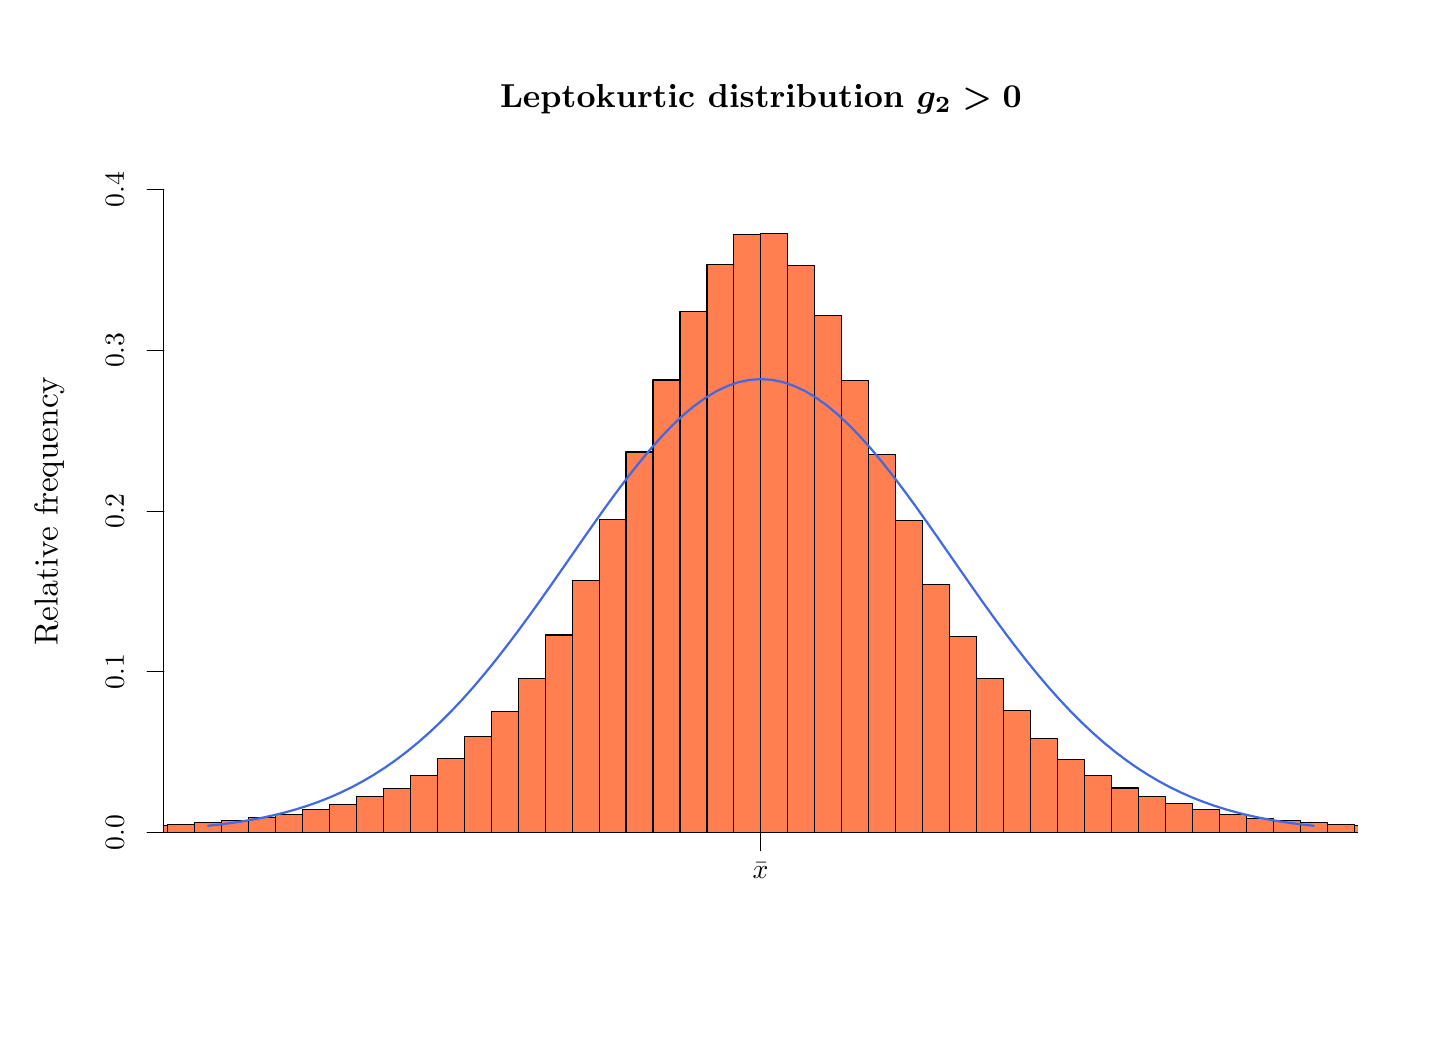
\begin{tikzpicture}[x=1pt,y=1pt]
\definecolor{fillColor}{RGB}{255,255,255}
\path[use as bounding box,fill=fillColor,fill opacity=0.00] (0,0) rectangle (505.89,361.35);
\begin{scope}
\path[clip] (  0.00,  0.00) rectangle (505.89,361.35);
\definecolor{drawColor}{RGB}{0,0,0}

\node[text=drawColor,anchor=base,inner sep=0pt, outer sep=0pt, scale=  1.20, font=\boldmath] at (264.94,332.61)
{\bfseries Leptokurtic distribution $g_2>0$};

\node[text=drawColor,rotate= 90.00,anchor=base,inner sep=0pt, outer sep=0pt, scale=  1.20] at ( 10.80,186.67)
{Relative frequency};
\end{scope}
\begin{scope}
\path[clip] ( 49.20, 61.20) rectangle (480.69,312.15);
\definecolor{drawColor}{RGB}{0,0,0}
\definecolor{fillColor}{RGB}{255,127,80}

\path[draw=drawColor,line width= 0.4pt,line join=round,line cap=round,fill=fillColor] ( -7.90, 70.49) rectangle (  1.84, 71.43);

\path[draw=drawColor,line width= 0.4pt,line join=round,line cap=round,fill=fillColor] (  1.84, 70.49) rectangle ( 11.59, 71.73);

\path[draw=drawColor,line width= 0.4pt,line join=round,line cap=round,fill=fillColor] ( 11.59, 70.49) rectangle ( 21.33, 71.97);

\path[draw=drawColor,line width= 0.4pt,line join=round,line cap=round,fill=fillColor] ( 21.33, 70.49) rectangle ( 31.08, 72.32);

\path[draw=drawColor,line width= 0.4pt,line join=round,line cap=round,fill=fillColor] ( 31.08, 70.49) rectangle ( 40.82, 72.61);

\path[draw=drawColor,line width= 0.4pt,line join=round,line cap=round,fill=fillColor] ( 40.82, 70.49) rectangle ( 50.56, 72.95);

\path[draw=drawColor,line width= 0.4pt,line join=round,line cap=round,fill=fillColor] ( 50.56, 70.49) rectangle ( 60.31, 73.34);

\path[draw=drawColor,line width= 0.4pt,line join=round,line cap=round,fill=fillColor] ( 60.31, 70.49) rectangle ( 70.05, 74.05);

\path[draw=drawColor,line width= 0.4pt,line join=round,line cap=round,fill=fillColor] ( 70.05, 70.49) rectangle ( 79.80, 74.81);

\path[draw=drawColor,line width= 0.4pt,line join=round,line cap=round,fill=fillColor] ( 79.80, 70.49) rectangle ( 89.54, 75.86);

\path[draw=drawColor,line width= 0.4pt,line join=round,line cap=round,fill=fillColor] ( 89.54, 70.49) rectangle ( 99.29, 77.18);

\path[draw=drawColor,line width= 0.4pt,line join=round,line cap=round,fill=fillColor] ( 99.29, 70.49) rectangle (109.03, 78.74);

\path[draw=drawColor,line width= 0.4pt,line join=round,line cap=round,fill=fillColor] (109.03, 70.49) rectangle (118.78, 80.76);

\path[draw=drawColor,line width= 0.4pt,line join=round,line cap=round,fill=fillColor] (118.78, 70.49) rectangle (128.52, 83.39);

\path[draw=drawColor,line width= 0.4pt,line join=round,line cap=round,fill=fillColor] (128.52, 70.49) rectangle (138.27, 86.54);

\path[draw=drawColor,line width= 0.4pt,line join=round,line cap=round,fill=fillColor] (138.27, 70.49) rectangle (148.01, 91.02);

\path[draw=drawColor,line width= 0.4pt,line join=round,line cap=round,fill=fillColor] (148.01, 70.49) rectangle (157.75, 97.14);

\path[draw=drawColor,line width= 0.4pt,line join=round,line cap=round,fill=fillColor] (157.75, 70.49) rectangle (167.50,105.09);

\path[draw=drawColor,line width= 0.4pt,line join=round,line cap=round,fill=fillColor] (167.50, 70.49) rectangle (177.24,114.25);

\path[draw=drawColor,line width= 0.4pt,line join=round,line cap=round,fill=fillColor] (177.24, 70.49) rectangle (186.99,126.25);

\path[draw=drawColor,line width= 0.4pt,line join=round,line cap=round,fill=fillColor] (186.99, 70.49) rectangle (196.73,141.90);

\path[draw=drawColor,line width= 0.4pt,line join=round,line cap=round,fill=fillColor] (196.73, 70.49) rectangle (206.48,161.66);

\path[draw=drawColor,line width= 0.4pt,line join=round,line cap=round,fill=fillColor] (206.48, 70.49) rectangle (216.22,183.76);

\path[draw=drawColor,line width= 0.4pt,line join=round,line cap=round,fill=fillColor] (216.22, 70.49) rectangle (225.97,208.02);

\path[draw=drawColor,line width= 0.4pt,line join=round,line cap=round,fill=fillColor] (225.97, 70.49) rectangle (235.71,234.04);

\path[draw=drawColor,line width= 0.4pt,line join=round,line cap=round,fill=fillColor] (235.71, 70.49) rectangle (245.46,258.92);

\path[draw=drawColor,line width= 0.4pt,line join=round,line cap=round,fill=fillColor] (245.46, 70.49) rectangle (255.20,275.69);

\path[draw=drawColor,line width= 0.4pt,line join=round,line cap=round,fill=fillColor] (255.20, 70.49) rectangle (264.94,286.56);

\path[draw=drawColor,line width= 0.4pt,line join=round,line cap=round,fill=fillColor] (264.94, 70.49) rectangle (274.69,286.83);

\path[draw=drawColor,line width= 0.4pt,line join=round,line cap=round,fill=fillColor] (274.69, 70.49) rectangle (284.43,275.51);

\path[draw=drawColor,line width= 0.4pt,line join=round,line cap=round,fill=fillColor] (284.43, 70.49) rectangle (294.18,257.22);

\path[draw=drawColor,line width= 0.4pt,line join=round,line cap=round,fill=fillColor] (294.18, 70.49) rectangle (303.92,233.82);

\path[draw=drawColor,line width= 0.4pt,line join=round,line cap=round,fill=fillColor] (303.92, 70.49) rectangle (313.67,207.22);

\path[draw=drawColor,line width= 0.4pt,line join=round,line cap=round,fill=fillColor] (313.67, 70.49) rectangle (323.41,183.13);

\path[draw=drawColor,line width= 0.4pt,line join=round,line cap=round,fill=fillColor] (323.41, 70.49) rectangle (333.16,160.21);

\path[draw=drawColor,line width= 0.4pt,line join=round,line cap=round,fill=fillColor] (333.16, 70.49) rectangle (342.90,141.38);

\path[draw=drawColor,line width= 0.4pt,line join=round,line cap=round,fill=fillColor] (342.90, 70.49) rectangle (352.65,126.27);

\path[draw=drawColor,line width= 0.4pt,line join=round,line cap=round,fill=fillColor] (352.65, 70.49) rectangle (362.39,114.52);

\path[draw=drawColor,line width= 0.4pt,line join=round,line cap=round,fill=fillColor] (362.39, 70.49) rectangle (372.14,104.42);

\path[draw=drawColor,line width= 0.4pt,line join=round,line cap=round,fill=fillColor] (372.14, 70.49) rectangle (381.88, 96.87);

\path[draw=drawColor,line width= 0.4pt,line join=round,line cap=round,fill=fillColor] (381.88, 70.49) rectangle (391.62, 90.97);

\path[draw=drawColor,line width= 0.4pt,line join=round,line cap=round,fill=fillColor] (391.62, 70.49) rectangle (401.37, 86.61);

\path[draw=drawColor,line width= 0.4pt,line join=round,line cap=round,fill=fillColor] (401.37, 70.49) rectangle (411.11, 83.56);

\path[draw=drawColor,line width= 0.4pt,line join=round,line cap=round,fill=fillColor] (411.11, 70.49) rectangle (420.86, 80.92);

\path[draw=drawColor,line width= 0.4pt,line join=round,line cap=round,fill=fillColor] (420.86, 70.49) rectangle (430.60, 78.90);

\path[draw=drawColor,line width= 0.4pt,line join=round,line cap=round,fill=fillColor] (430.60, 70.49) rectangle (440.35, 77.13);

\path[draw=drawColor,line width= 0.4pt,line join=round,line cap=round,fill=fillColor] (440.35, 70.49) rectangle (450.09, 75.58);

\path[draw=drawColor,line width= 0.4pt,line join=round,line cap=round,fill=fillColor] (450.09, 70.49) rectangle (459.84, 74.90);

\path[draw=drawColor,line width= 0.4pt,line join=round,line cap=round,fill=fillColor] (459.84, 70.49) rectangle (469.58, 73.98);

\path[draw=drawColor,line width= 0.4pt,line join=round,line cap=round,fill=fillColor] (469.58, 70.49) rectangle (479.33, 73.42);

\path[draw=drawColor,line width= 0.4pt,line join=round,line cap=round,fill=fillColor] (479.33, 70.49) rectangle (489.07, 72.92);

\path[draw=drawColor,line width= 0.4pt,line join=round,line cap=round,fill=fillColor] (489.07, 70.49) rectangle (498.81, 72.51);

\path[draw=drawColor,line width= 0.4pt,line join=round,line cap=round,fill=fillColor] (498.81, 70.49) rectangle (508.56, 72.10);
\end{scope}
\begin{scope}
\path[clip] (  0.00,  0.00) rectangle (505.89,361.35);
\definecolor{drawColor}{RGB}{0,0,0}

\path[draw=drawColor,line width= 0.4pt,line join=round,line cap=round] (264.79, 70.49) -- (264.79, 64);

\node[text=drawColor,anchor=base,inner sep=0pt, outer sep=0pt, scale=  1.00] at (264.79, 54) {$\bar x$};

\path[draw=drawColor,line width= 0.4pt,line join=round,line cap=round] ( 49.20, 70.49) -- ( 49.20,302.86);

\path[draw=drawColor,line width= 0.4pt,line join=round,line cap=round] ( 49.20, 70.49) -- ( 43.20, 70.49);

\path[draw=drawColor,line width= 0.4pt,line join=round,line cap=round] ( 49.20,128.58) -- ( 43.20,128.58);

\path[draw=drawColor,line width= 0.4pt,line join=round,line cap=round] ( 49.20,186.67) -- ( 43.20,186.67);

\path[draw=drawColor,line width= 0.4pt,line join=round,line cap=round] ( 49.20,244.77) -- ( 43.20,244.77);

\path[draw=drawColor,line width= 0.4pt,line join=round,line cap=round] ( 49.20,302.86) -- ( 43.20,302.86);

\node[text=drawColor,rotate= 90.00,anchor=base,inner sep=0pt, outer sep=0pt, scale=  1.00] at ( 34.80, 70.49) {0.0};

\node[text=drawColor,rotate= 90.00,anchor=base,inner sep=0pt, outer sep=0pt, scale=  1.00] at ( 34.80,128.58) {0.1};

\node[text=drawColor,rotate= 90.00,anchor=base,inner sep=0pt, outer sep=0pt, scale=  1.00] at ( 34.80,186.67) {0.2};

\node[text=drawColor,rotate= 90.00,anchor=base,inner sep=0pt, outer sep=0pt, scale=  1.00] at ( 34.80,244.77) {0.3};

\node[text=drawColor,rotate= 90.00,anchor=base,inner sep=0pt, outer sep=0pt, scale=  1.00] at ( 34.80,302.86) {0.4};
\end{scope}
\begin{scope}
\path[clip] ( 49.20, 61.20) rectangle (480.69,312.15);
\definecolor{drawColor}{RGB}{65,105,225}

\path[draw=drawColor,line width= 0.8pt,line join=round,line cap=round] ( 65.18, 72.95) --
	( 69.18, 73.39) --
	( 73.17, 73.90) --
	( 77.17, 74.49) --
	( 81.16, 75.17) --
	( 85.16, 75.94) --
	( 89.15, 76.82) --
	( 93.15, 77.82) --
	( 97.14, 78.94) --
	(101.14, 80.21) --
	(105.13, 81.62) --
	(109.13, 83.20) --
	(113.12, 84.96) --
	(117.12, 86.90) --
	(121.11, 89.04) --
	(125.11, 91.40) --
	(129.11, 93.97) --
	(133.10, 96.77) --
	(137.10, 99.80) --
	(141.09,103.07) --
	(145.09,106.59) --
	(149.08,110.35) --
	(153.08,114.36) --
	(157.07,118.61) --
	(161.07,123.09) --
	(165.06,127.80) --
	(169.06,132.72) --
	(173.05,137.84) --
	(177.05,143.13) --
	(181.04,148.58) --
	(185.04,154.15) --
	(189.03,159.81) --
	(193.03,165.55) --
	(197.03,171.31) --
	(201.02,177.06) --
	(205.02,182.76) --
	(209.01,188.37) --
	(213.01,193.84) --
	(217.00,199.13) --
	(221.00,204.20) --
	(224.99,209.01) --
	(228.99,213.50) --
	(232.98,217.65) --
	(236.98,221.41) --
	(240.97,224.74) --
	(244.97,227.62) --
	(248.96,230.02) --
	(252.96,231.90) --
	(256.95,233.27) --
	(260.95,234.09) --
	(264.94,234.36) --
	(268.94,234.09) --
	(272.94,233.27) --
	(276.93,231.90) --
	(280.93,230.02) --
	(284.92,227.62) --
	(288.92,224.74) --
	(292.91,221.41) --
	(296.91,217.65) --
	(300.90,213.50) --
	(304.90,209.01) --
	(308.89,204.20) --
	(312.89,199.13) --
	(316.88,193.84) --
	(320.88,188.37) --
	(324.87,182.76) --
	(328.87,177.06) --
	(332.86,171.31) --
	(336.86,165.55) --
	(340.86,159.81) --
	(344.85,154.15) --
	(348.85,148.58) --
	(352.84,143.13) --
	(356.84,137.84) --
	(360.83,132.72) --
	(364.83,127.80) --
	(368.82,123.09) --
	(372.82,118.61) --
	(376.81,114.36) --
	(380.81,110.35) --
	(384.80,106.59) --
	(388.80,103.07) --
	(392.79, 99.80) --
	(396.79, 96.77) --
	(400.78, 93.97) --
	(404.78, 91.40) --
	(408.77, 89.04) --
	(412.77, 86.90) --
	(416.77, 84.96) --
	(420.76, 83.20) --
	(424.76, 81.62) --
	(428.75, 80.21) --
	(432.75, 78.94) --
	(436.74, 77.82) --
	(440.74, 76.82) --
	(444.73, 75.94) --
	(448.73, 75.17) --
	(452.72, 74.49) --
	(456.72, 73.90) --
	(460.71, 73.39) --
	(464.71, 72.95);
\end{scope}
\end{tikzpicture}
}
\end{center} 
\end{frame}


%---------------------------------------------------------------------slide----
\begin{frame}
\frametitle{Coefficient of kurtosis}
\framesubtitle{Example with grouped data}
Using the frequency table of the sample with the heights of students and adding a new column with the deviations to
the mean $\bar x = 174.67$ cm to the fourth power, we get
\[
\setlength\arraycolsep{3mm}
\setlength\arrayrulewidth{0.5pt}
\begin{array}{rrrrr}
\hline
\multicolumn{1}{c}{X} & \multicolumn{1}{c}{x_i} & \multicolumn{1}{c}{n_i} & \multicolumn{1}{c}{x_i-\bar x} & \multicolumn{1}{c}{(x_i-\bar x)^4 n_i} \\
\hline
(150,160] & 155 & 2 & -19.67 & 299396.99\\
(160,170] & 165 & 8 & -9.67 & 69951.31\\
(170,180] & 175 & 11 & 0.33 & 0.13\\
(180,190] & 185 & 7 & 10.33 & 79707.53\\
(190,200] & 195 & 2 & 20.33 & 341648.49\\
\hline
\sum &  & 30 & & 790704.45 \\
\hline
\end{array}
\]
\[
g_2 = \frac{\sum (x_i-\bar x)^4n_i/n}{s^4} - 3 = \frac{790704.45/30}{10.1^4}-3 = -0.47.
\]
As it is a negative value but not too far from 0, that means that the distribution of heights is a little
bit platykurtic.
\end{frame}


%---------------------------------------------------------------------slide----
\begin{frame}
\frametitle{Interpretation }
As we will see in the chapters of inferential statistics, many of the statistical test can only be applied to normal
(bell-shaped) populations. 

Normal distributions are symmetrical and mesokurtic, and therefore, they have both the coefficients of symmetry and
kurtosis 0. So, a way of checking if a sample comes from a normal population is looking how far are the coefficients of
skewness and kurtosis from 0. 
 
In general, the normality of population is rejected when $g_1$ or $g_2$ are outside the interval $[-2,2]$.

In that case, is common to apply a transformation to the variable to correct non-normality. 
\end{frame}


\subsection{Variable transformations}

%---------------------------------------------------------------------slide----
\begin{frame}
\frametitle{Variable transformations}
\small
In many cases, the raw sample data are transformed to correct non-normality of distribution or just to get a more
appropriate scale.

For example, if we are working with heights in metres and a sample contains the following values:
\begin{center}
$1.75$ m, $1.65$ m, $1.80$ m,
\end{center}
it's possible to avoid decimals multiplying by 100, that is, changing from metres to centimetres:
\begin{center}
175 cm, 165 cm, 180 cm,
\end{center}
And it's also possible to reduce the magnitude of data subtracting the minimum value in the sample, in this case 165 cm:
\begin{center}
10 cm, 0 cm, 15 cm,
\end{center}
It's obvious that these data are easier to work with than the original ones.
In essences, what it's been done is to apply the following transformation o data:
\[Y= 100X-165\]
\end{frame}


%---------------------------------------------------------------------slide----
\begin{frame}
\frametitle{Linear transformations}
One of the most common transformations is a \emph{linear transformation}:
\[
Y=a+bX.
\]

For a linear transformation the mean and the standard deviation of the transformed variable are
\begin{align*}
\bar y &= a+ b\bar x,\\
s_{y} &= |b|s_{x}
\end{align*}

Additionally, the coefficient of kurtosis doesn't change and the coefficient of skewness changes only the sign if $b$ is
negative.
\end{frame}


%---------------------------------------------------------------------slide----
\begin{frame}
\frametitle{Standardization and standard scores}
One of the most common linear transformations is the \emph{standardization}.
\begin{definition}[Standardized variable and standard scores]
The \emph{standardized variable} of a variable $X$ is the variable that result of subtracting the mean from $X$ and
dividing by the standard deviation 
\[
Z=\frac{X-\bar x}{s_{x}}.
\]
For each value $x_i$ of the sample, the \emph{standard score} is the value that results of applying the standardization
transformation
\[
z_i=\frac{x_i-\bar x}{s_{x}}.
\]
\end{definition}

The standard score is the number of standard deviations a value is above or below the mean, and it's useful to avoid
the dependency of the variable from its measurement units.

The standardized variable always have mean 0 and standard deviation 1.  
\[
\bar z = 0 \qquad s_{z} = 1
\]
\end{frame}


%---------------------------------------------------------------------slide----
\begin{frame}
\frametitle{Standardization and standard scores}
\framesubtitle{Example}
The grades of 5 students in 2 subjects are
\[
\begin{array}{rccccccccc}
\mbox{Student:} & 1 & 2 & 3 & 4 & 5\\ \cline{1-6}
X: & 2 & 5 & 4 & \alert{8} & 6 & \qquad & \bar x = 5 & \quad s_x = 2\\
Y: & 1 & 9 & \alert{8} & 5 & 2 & \qquad & \bar y = 5 & \quad s_y = 3.16\\
\end{array}
\]
\begin{center}
\emph{Did the fourth student get the same performance in subject $X$ than the third student in subject $Y$?}
\end{center}
It might seem that both students had the same performance in every subject because they have the same
degree, but in order to get the performance of every student relative to the group of students, the dispersion
of grades in every subject must be considered.
For that reason is better to use the standard score as a measure of relative performance. 
\[
\begin{array}{cccccc}
X: & -1.5 & 0 & -0.5 & \alert{1.5} & 0.5 \\
Y: & -1.26 & 1.26 & \alert{0.95} & 0 & -0.95\\
\end{array}
\]
That is, the student with an 8 in $X$ is $1.5$ times the standard deviation below the mean of $X$, while the student
with an 8 in $Y$ is only $0.95$ times the standard deviation below the mean of $Y$. 
Therefore, the first student had a higher performance in $X$ than the second in $Y$.
\end{frame}


%---------------------------------------------------------------------slide----
\begin{frame}
\frametitle{Standardization and standard scores}
\framesubtitle{Example}
Following with the previous example and considering both subjects,
\begin{center}
\emph{which is the best student?}
\end{center}
If we only consider the sum of grades
\[
\begin{array}{rccccc}
\mbox{Student:} & 1 & 2 & 3 & 4 & 5\\ \hline
X: & 2 & 5 & 4 & 8 & 6 \\
Y: & 1 & 9 & 8 & 5 & 2 \\ \hline
\sum & 3 & \alert{14} & 12 & 13 & 8
\end{array}
\]
the best student is the second one. 

But if the relative performance is considered, taking the standard scores 
\[
\begin{array}{rccccc}
\mbox{Student:} & 1 & 2 & 3 & 4 & 5\\ \hline
X: & -1.5 & 0 & -0.5 & 1.5 & 0.5 \\
Y: & -1.26 & 1.26 & 0.95 & 0 & -0.95\\ \hline
\sum & -2.76 & 1.26 & 0.45 & \alert{1.5} & -0.45
\end{array}
\]
the best student is the fourth one. 
\end{frame}


%---------------------------------------------------------------------slide----
\begin{frame}
\frametitle{Non-linear transformations}
Non-linear transformations are also common to correct non-normality of distributions.

The square transformation $Y=X^2$ compresses small values and expand large values.
So, it's used to correct left-skewed distributions.

\begin{center}
\tikzsetnextfilename{descriptive/square_transformation}
\scalebox{0.4}{% Created by tikzDevice version 0.8.1 on 2015-11-21 19:12:36
% !TEX encoding = UTF-8 Unicode
\begin{tikzpicture}[x=1pt,y=1pt]
\begin{scope}[local bounding box=right,xscale=-1]
\path[clip] (  0.00,  0.00) rectangle (361.35,361.35);
\definecolor{drawColor}{RGB}{0,0,0}
\definecolor{fillColor}{RGB}{255,127,80}

\path[draw=drawColor,line width= 0.4pt,line join=round,line cap=round,fill=fillColor] ( 13.38, 13.38) rectangle ( 22.75, 33.39);

\path[draw=drawColor,line width= 0.4pt,line join=round,line cap=round,fill=fillColor] ( 22.75, 13.38) rectangle ( 32.12,147.95);

\path[draw=drawColor,line width= 0.4pt,line join=round,line cap=round,fill=fillColor] ( 32.12, 13.38) rectangle ( 41.49,272.26);

\path[draw=drawColor,line width= 0.4pt,line join=round,line cap=round,fill=fillColor] ( 41.49, 13.38) rectangle ( 50.86,333.61);

\path[draw=drawColor,line width= 0.4pt,line join=round,line cap=round,fill=fillColor] ( 50.86, 13.38) rectangle ( 60.22,347.97);

\path[draw=drawColor,line width= 0.4pt,line join=round,line cap=round,fill=fillColor] ( 60.22, 13.38) rectangle ( 69.59,330.96);

\path[draw=drawColor,line width= 0.4pt,line join=round,line cap=round,fill=fillColor] ( 69.59, 13.38) rectangle ( 78.96,297.52);

\path[draw=drawColor,line width= 0.4pt,line join=round,line cap=round,fill=fillColor] ( 78.96, 13.38) rectangle ( 88.33,262.02);

\path[draw=drawColor,line width= 0.4pt,line join=round,line cap=round,fill=fillColor] ( 88.33, 13.38) rectangle ( 97.70,224.79);

\path[draw=drawColor,line width= 0.4pt,line join=round,line cap=round,fill=fillColor] ( 97.70, 13.38) rectangle (107.07,194.77);

\path[draw=drawColor,line width= 0.4pt,line join=round,line cap=round,fill=fillColor] (107.07, 13.38) rectangle (116.43,167.49);

\path[draw=drawColor,line width= 0.4pt,line join=round,line cap=round,fill=fillColor] (116.43, 13.38) rectangle (125.80,143.13);

\path[draw=drawColor,line width= 0.4pt,line join=round,line cap=round,fill=fillColor] (125.80, 13.38) rectangle (135.17,123.83);

\path[draw=drawColor,line width= 0.4pt,line join=round,line cap=round,fill=fillColor] (135.17, 13.38) rectangle (144.54,106.27);

\path[draw=drawColor,line width= 0.4pt,line join=round,line cap=round,fill=fillColor] (144.54, 13.38) rectangle (153.91, 92.51);

\path[draw=drawColor,line width= 0.4pt,line join=round,line cap=round,fill=fillColor] (153.91, 13.38) rectangle (163.28, 80.87);

\path[draw=drawColor,line width= 0.4pt,line join=round,line cap=round,fill=fillColor] (163.28, 13.38) rectangle (172.64, 70.81);

\path[draw=drawColor,line width= 0.4pt,line join=round,line cap=round,fill=fillColor] (172.64, 13.38) rectangle (182.01, 63.16);

\path[draw=drawColor,line width= 0.4pt,line join=round,line cap=round,fill=fillColor] (182.01, 13.38) rectangle (191.38, 55.12);

\path[draw=drawColor,line width= 0.4pt,line join=round,line cap=round,fill=fillColor] (191.38, 13.38) rectangle (200.75, 49.22);

\path[draw=drawColor,line width= 0.4pt,line join=round,line cap=round,fill=fillColor] (200.75, 13.38) rectangle (210.12, 45.41);

\path[draw=drawColor,line width= 0.4pt,line join=round,line cap=round,fill=fillColor] (210.12, 13.38) rectangle (219.49, 40.63);

\path[draw=drawColor,line width= 0.4pt,line join=round,line cap=round,fill=fillColor] (219.49, 13.38) rectangle (228.85, 37.65);

\path[draw=drawColor,line width= 0.4pt,line join=round,line cap=round,fill=fillColor] (228.85, 13.38) rectangle (238.22, 33.70);

\path[draw=drawColor,line width= 0.4pt,line join=round,line cap=round,fill=fillColor] (238.22, 13.38) rectangle (247.59, 31.31);

\path[draw=drawColor,line width= 0.4pt,line join=round,line cap=round,fill=fillColor] (247.59, 13.38) rectangle (256.96, 29.38);

\path[draw=drawColor,line width= 0.4pt,line join=round,line cap=round,fill=fillColor] (256.96, 13.38) rectangle (266.33, 27.29);

\path[draw=drawColor,line width= 0.4pt,line join=round,line cap=round,fill=fillColor] (266.33, 13.38) rectangle (275.70, 25.70);

\path[draw=drawColor,line width= 0.4pt,line join=round,line cap=round,fill=fillColor] (275.70, 13.38) rectangle (285.06, 24.31);

\path[draw=drawColor,line width= 0.4pt,line join=round,line cap=round,fill=fillColor] (285.06, 13.38) rectangle (294.43, 22.93);

\path[draw=drawColor,line width= 0.4pt,line join=round,line cap=round,fill=fillColor] (294.43, 13.38) rectangle (303.80, 22.37);

\path[draw=drawColor,line width= 0.4pt,line join=round,line cap=round,fill=fillColor] (303.80, 13.38) rectangle (313.17, 21.26);

\path[draw=drawColor,line width= 0.4pt,line join=round,line cap=round,fill=fillColor] (313.17, 13.38) rectangle (322.54, 20.07);

\path[draw=drawColor,line width= 0.4pt,line join=round,line cap=round,fill=fillColor] (322.54, 13.38) rectangle (331.91, 19.63);

\path[draw=drawColor,line width= 0.4pt,line join=round,line cap=round,fill=fillColor] (331.91, 13.38) rectangle (341.27, 19.31);

\path[draw=drawColor,line width= 0.4pt,line join=round,line cap=round,fill=fillColor] (341.27, 13.38) rectangle (350.64, 18.45);

\path[draw=drawColor,line width= 0.4pt,line join=round,line cap=round,fill=fillColor] (350.64, 13.38) rectangle (360.01, 17.82);

\path[draw=drawColor,line width= 0.4pt,line join=round,line cap=round,fill=fillColor] (360.01, 13.38) rectangle (369.38, 17.41);
\end{scope}

\node at (right.east) [xshift=2cm, fill=color1,single arrow,shape border rotate=0,text=white, minimum width=2cm]{\huge\
$Y=X^2$\ \phantom{}};

\begin{scope}[xshift=3cm]
\path[clip] (  0.00,  0.00) rectangle (361.35,361.35);
\definecolor{drawColor}{RGB}{0,0,0}
\definecolor{fillColor}{RGB}{255,127,80}

\path[draw=drawColor,line width= 0.4pt,line join=round,line cap=round,fill=fillColor] ( -3.77, 13.38) rectangle (  5.79, 13.68);

\path[draw=drawColor,line width= 0.4pt,line join=round,line cap=round,fill=fillColor] (  5.79, 13.38) rectangle ( 15.35, 13.89);

\path[draw=drawColor,line width= 0.4pt,line join=round,line cap=round,fill=fillColor] ( 15.35, 13.38) rectangle ( 24.91, 14.55);

\path[draw=drawColor,line width= 0.4pt,line join=round,line cap=round,fill=fillColor] ( 24.91, 13.38) rectangle ( 34.46, 15.89);

\path[draw=drawColor,line width= 0.4pt,line join=round,line cap=round,fill=fillColor] ( 34.46, 13.38) rectangle ( 44.02, 17.63);

\path[draw=drawColor,line width= 0.4pt,line join=round,line cap=round,fill=fillColor] ( 44.02, 13.38) rectangle ( 53.58, 20.81);

\path[draw=drawColor,line width= 0.4pt,line join=round,line cap=round,fill=fillColor] ( 53.58, 13.38) rectangle ( 63.14, 25.99);

\path[draw=drawColor,line width= 0.4pt,line join=round,line cap=round,fill=fillColor] ( 63.14, 13.38) rectangle ( 72.70, 33.85);

\path[draw=drawColor,line width= 0.4pt,line join=round,line cap=round,fill=fillColor] ( 72.70, 13.38) rectangle ( 82.26, 45.35);

\path[draw=drawColor,line width= 0.4pt,line join=round,line cap=round,fill=fillColor] ( 82.26, 13.38) rectangle ( 91.82, 63.02);

\path[draw=drawColor,line width= 0.4pt,line join=round,line cap=round,fill=fillColor] ( 91.82, 13.38) rectangle (101.38, 84.64);

\path[draw=drawColor,line width= 0.4pt,line join=round,line cap=round,fill=fillColor] (101.38, 13.38) rectangle (110.94,113.77);

\path[draw=drawColor,line width= 0.4pt,line join=round,line cap=round,fill=fillColor] (110.94, 13.38) rectangle (120.50,145.73);

\path[draw=drawColor,line width= 0.4pt,line join=round,line cap=round,fill=fillColor] (120.50, 13.38) rectangle (130.06,182.51);

\path[draw=drawColor,line width= 0.4pt,line join=round,line cap=round,fill=fillColor] (130.06, 13.38) rectangle (139.62,224.97);

\path[draw=drawColor,line width= 0.4pt,line join=round,line cap=round,fill=fillColor] (139.62, 13.38) rectangle (149.18,262.67);

\path[draw=drawColor,line width= 0.4pt,line join=round,line cap=round,fill=fillColor] (149.18, 13.38) rectangle (158.74,298.41);

\path[draw=drawColor,line width= 0.4pt,line join=round,line cap=round,fill=fillColor] (158.74, 13.38) rectangle (168.30,325.16);

\path[draw=drawColor,line width= 0.4pt,line join=round,line cap=round,fill=fillColor] (168.30, 13.38) rectangle (177.86,343.18);

\path[draw=drawColor,line width= 0.4pt,line join=round,line cap=round,fill=fillColor] (177.86, 13.38) rectangle (187.42,346.32);

\path[draw=drawColor,line width= 0.4pt,line join=round,line cap=round,fill=fillColor] (187.42, 13.38) rectangle (196.98,337.54);

\path[draw=drawColor,line width= 0.4pt,line join=round,line cap=round,fill=fillColor] (196.98, 13.38) rectangle (206.54,315.93);

\path[draw=drawColor,line width= 0.4pt,line join=round,line cap=round,fill=fillColor] (206.54, 13.38) rectangle (216.10,285.51);

\path[draw=drawColor,line width= 0.4pt,line join=round,line cap=round,fill=fillColor] (216.10, 13.38) rectangle (225.66,246.57);

\path[draw=drawColor,line width= 0.4pt,line join=round,line cap=round,fill=fillColor] (225.66, 13.38) rectangle (235.21,207.81);

\path[draw=drawColor,line width= 0.4pt,line join=round,line cap=round,fill=fillColor] (235.21, 13.38) rectangle (244.77,169.39);

\path[draw=drawColor,line width= 0.4pt,line join=round,line cap=round,fill=fillColor] (244.77, 13.38) rectangle (254.33,131.11);

\path[draw=drawColor,line width= 0.4pt,line join=round,line cap=round,fill=fillColor] (254.33, 13.38) rectangle (263.89,100.53);

\path[draw=drawColor,line width= 0.4pt,line join=round,line cap=round,fill=fillColor] (263.89, 13.38) rectangle (273.45, 74.00);

\path[draw=drawColor,line width= 0.4pt,line join=round,line cap=round,fill=fillColor] (273.45, 13.38) rectangle (283.01, 54.77);

\path[draw=drawColor,line width= 0.4pt,line join=round,line cap=round,fill=fillColor] (283.01, 13.38) rectangle (292.57, 41.02);

\path[draw=drawColor,line width= 0.4pt,line join=round,line cap=round,fill=fillColor] (292.57, 13.38) rectangle (302.13, 30.76);

\path[draw=drawColor,line width= 0.4pt,line join=round,line cap=round,fill=fillColor] (302.13, 13.38) rectangle (311.69, 23.88);

\path[draw=drawColor,line width= 0.4pt,line join=round,line cap=round,fill=fillColor] (311.69, 13.38) rectangle (321.25, 19.33);

\path[draw=drawColor,line width= 0.4pt,line join=round,line cap=round,fill=fillColor] (321.25, 13.38) rectangle (330.81, 16.84);

\path[draw=drawColor,line width= 0.4pt,line join=round,line cap=round,fill=fillColor] (330.81, 13.38) rectangle (340.37, 15.15);

\path[draw=drawColor,line width= 0.4pt,line join=round,line cap=round,fill=fillColor] (340.37, 13.38) rectangle (349.93, 14.30);

\path[draw=drawColor,line width= 0.4pt,line join=round,line cap=round,fill=fillColor] (349.93, 13.38) rectangle (359.49, 13.77);

\path[draw=drawColor,line width= 0.4pt,line join=round,line cap=round,fill=fillColor] (359.49, 13.38) rectangle (369.05, 13.59);
\end{scope}

\end{tikzpicture}
}
\end{center} 
\end{frame}


%---------------------------------------------------------------------slide----
\begin{frame}
\frametitle{Non-linear transformation}
The square root transformation $Y=\sqrt x$, the logarithmic tranformation $Y= \log X$ and the inverse transformation
$Y=1/X$ compresses large values and expand small values.
So, they are used to correct right-skewed distributions. 
\begin{center}
\tikzsetnextfilename{descriptive/log_transformation}
\scalebox{0.4}{\input{img/descriptive/log_transformation}}
\end{center} 
\end{frame}


%---------------------------------------------------------------------slide----
\begin{frame}
\frametitle{Factors}
Sometimes is interesting to describe the frequency distribution of the main variable for different subsamples
corresponding to the categories of another variable that is known as \highlight{\textbf{classificatory variable}} or
\highlight{\textbf{factor}}.

\highlight{Example} Dividing the sample of heights by gender we get two subsamples
\begin{center}
\begin{tabular}{lll}
\hline
\multirow{2}{*}{Females} &
173, 158, 174, 166, 162, 177, 165, 154, 166, 182, \\
& 169, 172, 170, 168. \\
\hline
\multirow{2}{*}{Males} &
179, 181, 172, 194, 185, 187, 198, 178, 188, 171,\\
& 175, 167, 186, 172, 176, 187. \\
\hline
\end{tabular}
\end{center}
\end{frame}


%---------------------------------------------------------------------slide----
\begin{frame}
\frametitle{Comparing distributions for the levels of a factor }

\begin{center} 
\tikzsetnextfilename{descriptive/factor_histogram}
\scalebox{0.45}{% Created by tikzDevice version 0.8.1 on 2016-01-28 18:44:16
% !TEX encoding = UTF-8 Unicode
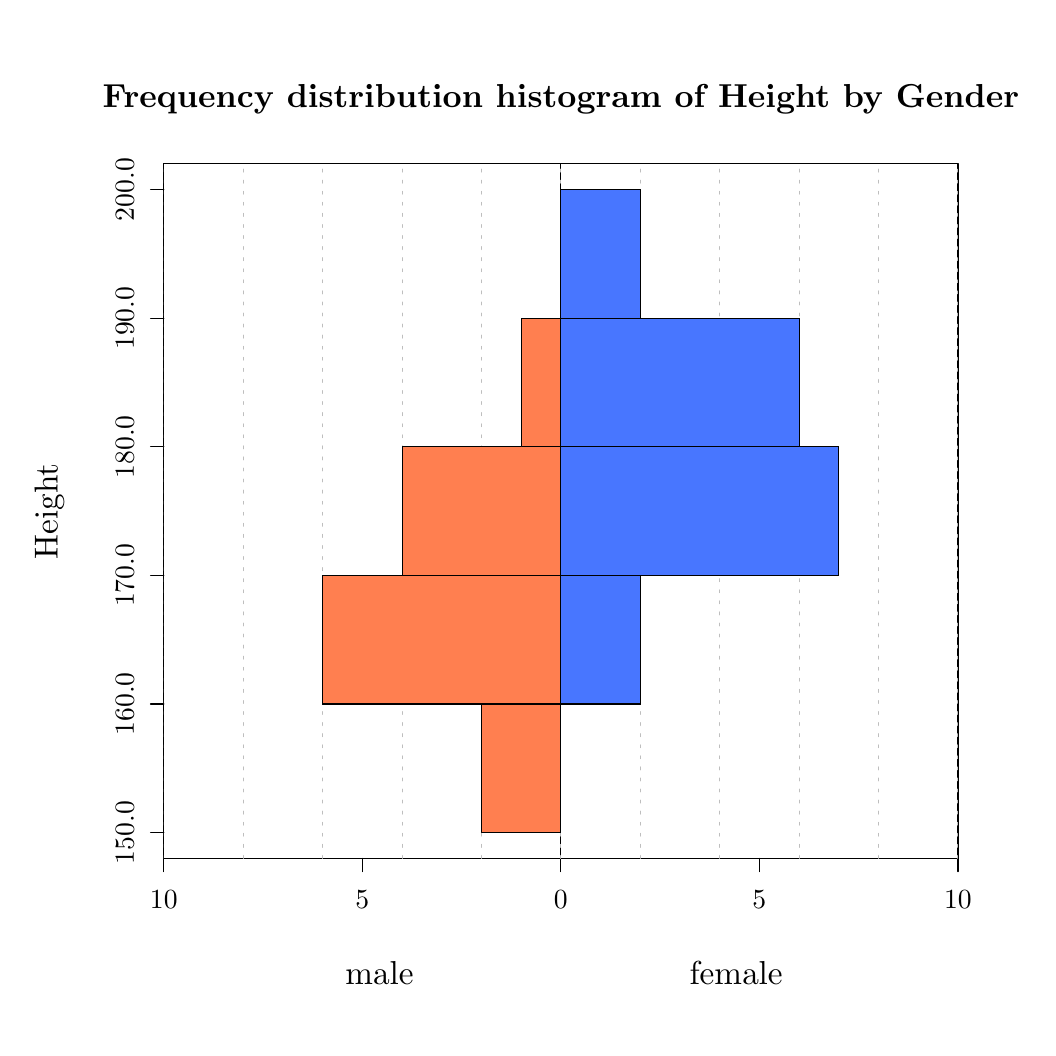
\begin{tikzpicture}[x=1pt,y=1pt]
\definecolor{fillColor}{RGB}{255,255,255}
\path[use as bounding box,fill=fillColor,fill opacity=0.00] (0,0) rectangle (361.35,361.35);
\begin{scope}
\path[clip] (  0.00,  0.00) rectangle (361.35,361.35);
\definecolor{drawColor}{RGB}{0,0,0}

\path[draw=drawColor,line width= 0.4pt,line join=round,line cap=round] (192.68, 70.49) rectangle (163.98,116.97);

\path[draw=drawColor,line width= 0.4pt,line join=round,line cap=round] (192.68,116.97) rectangle (106.59,163.44);

\path[draw=drawColor,line width= 0.4pt,line join=round,line cap=round] (192.68,163.44) rectangle (135.28,209.91);

\path[draw=drawColor,line width= 0.4pt,line join=round,line cap=round] (192.68,209.91) rectangle (178.33,256.38);

\path[draw=drawColor,line width= 0.4pt,line join=round,line cap=round] (192.68,256.38) rectangle (192.68,302.86);

\end{scope}
\begin{scope}
\path[clip] (  0.00,  0.00) rectangle (361.35,361.35);
\definecolor{drawColor}{RGB}{0,0,0}

\path[draw=drawColor,line width= 0.4pt,line join=round,line cap=round] (192.68, 70.49) rectangle (192.68,116.97);

\path[draw=drawColor,line width= 0.4pt,line join=round,line cap=round] (192.68,116.97) rectangle (221.37,163.44);

\path[draw=drawColor,line width= 0.4pt,line join=round,line cap=round] (192.68,163.44) rectangle (293.11,209.91);

\path[draw=drawColor,line width= 0.4pt,line join=round,line cap=round] (192.68,209.91) rectangle (278.76,256.38);

\path[draw=drawColor,line width= 0.4pt,line join=round,line cap=round] (192.68,256.38) rectangle (221.37,302.86);

\node[text=drawColor,anchor=base,inner sep=0pt, outer sep=0pt, scale=  1.20] at (192.68,332.61) {\bfseries Frequency distribution histogram of Height by Gender};
\end{scope}
\begin{scope}
\path[clip] (  0.00,  0.00) rectangle (361.35,361.35);
\definecolor{drawColor}{RGB}{0,0,0}

\path[draw=drawColor,line width= 0.4pt,line join=round,line cap=round] ( 49.20, 61.20) -- (336.15, 61.20);

\path[draw=drawColor,line width= 0.4pt,line join=round,line cap=round] ( 49.20, 61.20) -- ( 49.20, 56.40);

\path[draw=drawColor,line width= 0.4pt,line join=round,line cap=round] (120.94, 61.20) -- (120.94, 56.40);

\path[draw=drawColor,line width= 0.4pt,line join=round,line cap=round] (192.68, 61.20) -- (192.68, 56.40);

\path[draw=drawColor,line width= 0.4pt,line join=round,line cap=round] (264.41, 61.20) -- (264.41, 56.40);

\path[draw=drawColor,line width= 0.4pt,line join=round,line cap=round] (336.15, 61.20) -- (336.15, 56.40);

\node[text=drawColor,anchor=base,inner sep=0pt, outer sep=0pt, scale=  1.00] at ( 49.20, 43.20) {10};

\node[text=drawColor,anchor=base,inner sep=0pt, outer sep=0pt, scale=  1.00] at (120.94, 43.20) { 5};

\node[text=drawColor,anchor=base,inner sep=0pt, outer sep=0pt, scale=  1.00] at (192.68, 43.20) { 0};

\node[text=drawColor,anchor=base,inner sep=0pt, outer sep=0pt, scale=  1.00] at (264.41, 43.20) { 5};

\node[text=drawColor,anchor=base,inner sep=0pt, outer sep=0pt, scale=  1.00] at (336.15, 43.20) {10};

\path[draw=drawColor,line width= 0.4pt,line join=round,line cap=round] ( 49.20, 70.49) -- ( 49.20,302.86);

\path[draw=drawColor,line width= 0.4pt,line join=round,line cap=round] ( 49.20, 70.49) -- ( 44.40, 70.49);

\path[draw=drawColor,line width= 0.4pt,line join=round,line cap=round] ( 49.20,116.97) -- ( 44.40,116.97);

\path[draw=drawColor,line width= 0.4pt,line join=round,line cap=round] ( 49.20,163.44) -- ( 44.40,163.44);

\path[draw=drawColor,line width= 0.4pt,line join=round,line cap=round] ( 49.20,209.91) -- ( 44.40,209.91);

\path[draw=drawColor,line width= 0.4pt,line join=round,line cap=round] ( 49.20,256.38) -- ( 44.40,256.38);

\path[draw=drawColor,line width= 0.4pt,line join=round,line cap=round] ( 49.20,302.86) -- ( 44.40,302.86);

\node[text=drawColor,rotate= 90.00,anchor=base,inner sep=0pt, outer sep=0pt, scale=  1.00] at ( 38.40, 70.49) {150.0};

\node[text=drawColor,rotate= 90.00,anchor=base,inner sep=0pt, outer sep=0pt, scale=  1.00] at ( 38.40,116.97) {160.0};

\node[text=drawColor,rotate= 90.00,anchor=base,inner sep=0pt, outer sep=0pt, scale=  1.00] at ( 38.40,163.44) {170.0};

\node[text=drawColor,rotate= 90.00,anchor=base,inner sep=0pt, outer sep=0pt, scale=  1.00] at ( 38.40,209.91) {180.0};

\node[text=drawColor,rotate= 90.00,anchor=base,inner sep=0pt, outer sep=0pt, scale=  1.00] at ( 38.40,256.38) {190.0};

\node[text=drawColor,rotate= 90.00,anchor=base,inner sep=0pt, outer sep=0pt, scale=  1.00] at ( 38.40,302.86) {200.0};
\end{scope}
\begin{scope}
\path[clip] (  0.00,  0.00) rectangle (361.35,361.35);
\definecolor{drawColor}{RGB}{0,0,0}

\node[text=drawColor,anchor=base,inner sep=0pt, outer sep=0pt, scale=  1.20] at (127.10, 15.60) {male};

\node[text=drawColor,anchor=base east,inner sep=0pt, outer sep=0pt, scale=  1.20] at (272.83, 15.60) {female};

\node[text=drawColor,rotate= 90.00,anchor=base,inner sep=0pt, outer sep=0pt, scale=  1.20] at ( 10.80,186.67) {Height};
\end{scope}
\begin{scope}
\path[clip] ( 49.20, 61.20) rectangle (336.15,312.15);
\definecolor{drawColor}{RGB}{0,0,0}

\path[draw=drawColor,line width= 0.4pt,line join=round,line cap=round] (192.68, 61.20) -- (192.68,312.15);
\end{scope}
\begin{scope}
\path[clip] (  0.00,  0.00) rectangle (361.35,361.35);
\definecolor{drawColor}{RGB}{0,0,0}

\path[draw=drawColor,line width= 0.4pt,line join=round,line cap=round] ( 49.20, 61.20) --
	(336.15, 61.20) --
	(336.15,312.15) --
	( 49.20,312.15) --
	( 49.20, 61.20);
\end{scope}
\begin{scope}
\path[clip] ( 49.20, 61.20) rectangle (336.15,312.15);
\definecolor{drawColor}{RGB}{190,190,190}

\path[draw=drawColor,line width= 0.4pt,dash pattern=on 1pt off 3pt ,line join=round,line cap=round] ( 20.51, 61.20) -- ( 20.51,312.15);

\path[draw=drawColor,line width= 0.4pt,dash pattern=on 1pt off 3pt ,line join=round,line cap=round] ( 49.20, 61.20) -- ( 49.20,312.15);

\path[draw=drawColor,line width= 0.4pt,dash pattern=on 1pt off 3pt ,line join=round,line cap=round] ( 77.90, 61.20) -- ( 77.90,312.15);

\path[draw=drawColor,line width= 0.4pt,dash pattern=on 1pt off 3pt ,line join=round,line cap=round] (106.59, 61.20) -- (106.59,312.15);

\path[draw=drawColor,line width= 0.4pt,dash pattern=on 1pt off 3pt ,line join=round,line cap=round] (135.28, 61.20) -- (135.28,312.15);

\path[draw=drawColor,line width= 0.4pt,dash pattern=on 1pt off 3pt ,line join=round,line cap=round] (163.98, 61.20) -- (163.98,312.15);

\path[draw=drawColor,line width= 0.4pt,dash pattern=on 1pt off 3pt ,line join=round,line cap=round] (192.68, 61.20) -- (192.68,312.15);

\path[draw=drawColor,line width= 0.4pt,dash pattern=on 1pt off 3pt ,line join=round,line cap=round] (221.37, 61.20) -- (221.37,312.15);

\path[draw=drawColor,line width= 0.4pt,dash pattern=on 1pt off 3pt ,line join=round,line cap=round] (250.06, 61.20) -- (250.06,312.15);

\path[draw=drawColor,line width= 0.4pt,dash pattern=on 1pt off 3pt ,line join=round,line cap=round] (278.76, 61.20) -- (278.76,312.15);

\path[draw=drawColor,line width= 0.4pt,dash pattern=on 1pt off 3pt ,line join=round,line cap=round] (307.45, 61.20) -- (307.45,312.15);

\path[draw=drawColor,line width= 0.4pt,dash pattern=on 1pt off 3pt ,line join=round,line cap=round] (336.15, 61.20) -- (336.15,312.15);
\end{scope}
\begin{scope}
\path[clip] (  0.00,  0.00) rectangle (361.35,361.35);
\definecolor{drawColor}{RGB}{0,0,0}
\definecolor{fillColor}{RGB}{255,127,80}

\path[draw=drawColor,line width= 0.4pt,line join=round,line cap=round,fill=fillColor] (192.68, 70.49) rectangle (163.98,116.97);

\path[draw=drawColor,line width= 0.4pt,line join=round,line cap=round,fill=fillColor] (192.68,116.97) rectangle (106.59,163.44);

\path[draw=drawColor,line width= 0.4pt,line join=round,line cap=round,fill=fillColor] (192.68,163.44) rectangle (135.28,209.91);

\path[draw=drawColor,line width= 0.4pt,line join=round,line cap=round,fill=fillColor] (192.68,209.91) rectangle (178.33,256.38);

\path[draw=drawColor,line width= 0.4pt,line join=round,line cap=round,fill=fillColor] (192.68,256.38) rectangle (192.68,302.86);
\definecolor{fillColor}{RGB}{72,118,255}

\path[draw=drawColor,line width= 0.4pt,line join=round,line cap=round,fill=fillColor] (192.68, 70.49) rectangle (192.68,116.97);

\path[draw=drawColor,line width= 0.4pt,line join=round,line cap=round,fill=fillColor] (192.68,116.97) rectangle (221.37,163.44);

\path[draw=drawColor,line width= 0.4pt,line join=round,line cap=round,fill=fillColor] (192.68,163.44) rectangle (293.11,209.91);

\path[draw=drawColor,line width= 0.4pt,line join=round,line cap=round,fill=fillColor] (192.68,209.91) rectangle (278.76,256.38);

\path[draw=drawColor,line width= 0.4pt,line join=round,line cap=round,fill=fillColor] (192.68,256.38) rectangle (221.37,302.86);
\end{scope}
\end{tikzpicture}
}
\tikzsetnextfilename{descriptive/factor_box_plot}
\scalebox{0.45}{% Created by tikzDevice version 0.8.1 on 2016-01-28 18:51:29
% !TEX encoding = UTF-8 Unicode
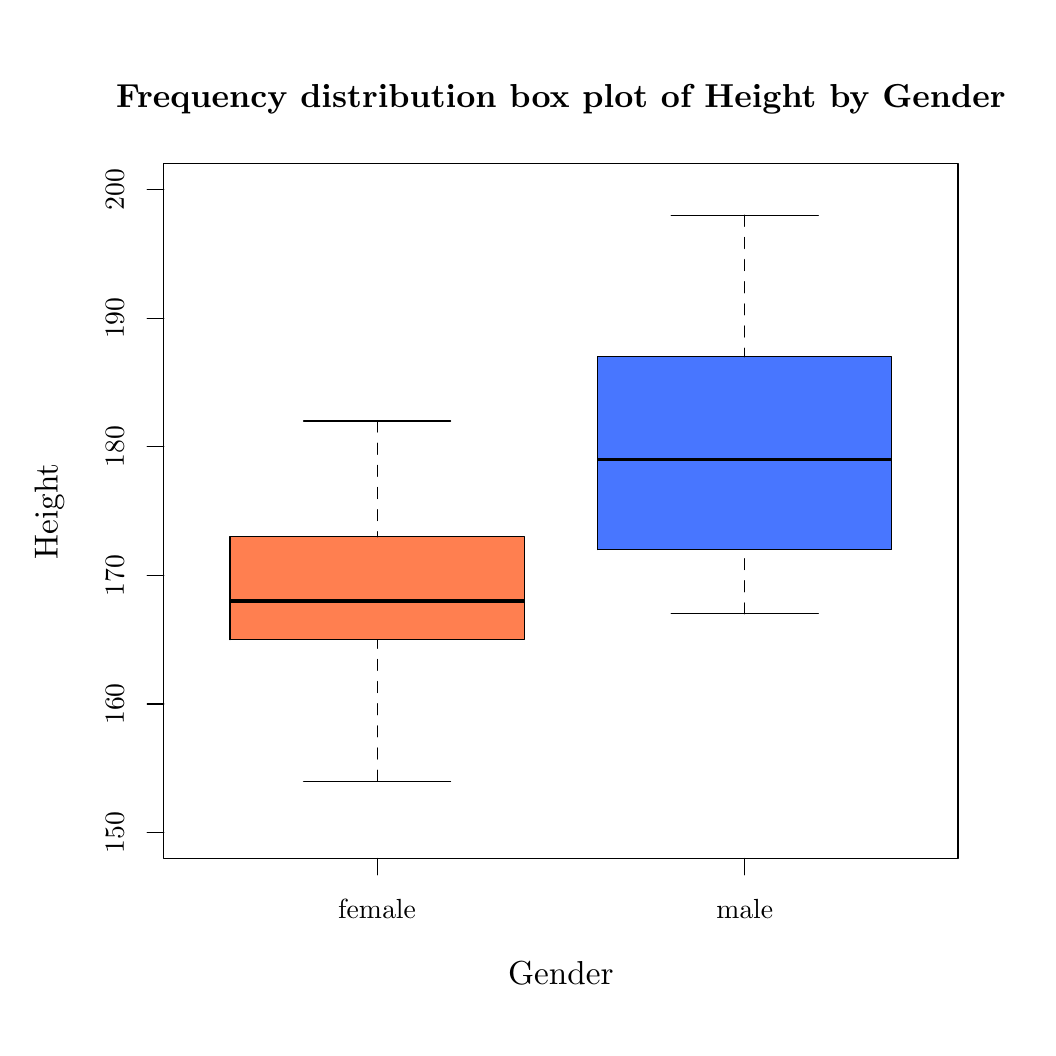
\begin{tikzpicture}[x=1pt,y=1pt]
\definecolor{fillColor}{RGB}{255,255,255}
\path[use as bounding box,fill=fillColor,fill opacity=0.00] (0,0) rectangle (361.35,361.35);
\begin{scope}
\path[clip] ( 49.20, 61.20) rectangle (336.15,312.15);
\definecolor{fillColor}{RGB}{255,127,80}

\path[fill=fillColor] ( 73.11,140.20) --
	(179.39,140.20) --
	(179.39,177.38) --
	( 73.11,177.38) --
	cycle;
\definecolor{drawColor}{RGB}{0,0,0}

\path[draw=drawColor,line width= 1.2pt,line join=round] ( 73.11,154.14) -- (179.39,154.14);

\path[draw=drawColor,line width= 0.4pt,dash pattern=on 4pt off 4pt ,line join=round,line cap=round] (126.25, 89.08) -- (126.25,140.20);

\path[draw=drawColor,line width= 0.4pt,dash pattern=on 4pt off 4pt ,line join=round,line cap=round] (126.25,219.21) -- (126.25,177.38);

\path[draw=drawColor,line width= 0.4pt,line join=round,line cap=round] ( 99.68, 89.08) -- (152.82, 89.08);

\path[draw=drawColor,line width= 0.4pt,line join=round,line cap=round] ( 99.68,219.21) -- (152.82,219.21);

\path[draw=drawColor,line width= 0.4pt,line join=round,line cap=round] ( 73.11,140.20) --
	(179.39,140.20) --
	(179.39,177.38) --
	( 73.11,177.38) --
	( 73.11,140.20);
\definecolor{fillColor}{RGB}{72,118,255}

\path[fill=fillColor] (205.96,172.73) --
	(312.24,172.73) --
	(312.24,242.44) --
	(205.96,242.44) --
	cycle;

\path[draw=drawColor,line width= 1.2pt,line join=round] (205.96,205.26) -- (312.24,205.26);

\path[draw=drawColor,line width= 0.4pt,dash pattern=on 4pt off 4pt ,line join=round,line cap=round] (259.10,149.50) -- (259.10,172.73);

\path[draw=drawColor,line width= 0.4pt,dash pattern=on 4pt off 4pt ,line join=round,line cap=round] (259.10,293.56) -- (259.10,242.44);

\path[draw=drawColor,line width= 0.4pt,line join=round,line cap=round] (232.53,149.50) -- (285.67,149.50);

\path[draw=drawColor,line width= 0.4pt,line join=round,line cap=round] (232.53,293.56) -- (285.67,293.56);

\path[draw=drawColor,line width= 0.4pt,line join=round,line cap=round] (205.96,172.73) --
	(312.24,172.73) --
	(312.24,242.44) --
	(205.96,242.44) --
	(205.96,172.73);
\end{scope}
\begin{scope}
\path[clip] (  0.00,  0.00) rectangle (361.35,361.35);
\definecolor{drawColor}{RGB}{0,0,0}

\path[draw=drawColor,line width= 0.4pt,line join=round,line cap=round] (126.25, 61.20) -- (259.10, 61.20);

\path[draw=drawColor,line width= 0.4pt,line join=round,line cap=round] (126.25, 61.20) -- (126.25, 55.20);

\path[draw=drawColor,line width= 0.4pt,line join=round,line cap=round] (259.10, 61.20) -- (259.10, 55.20);

\node[text=drawColor,anchor=base,inner sep=0pt, outer sep=0pt, scale=  1.00] at (126.25, 39.60) {female};

\node[text=drawColor,anchor=base,inner sep=0pt, outer sep=0pt, scale=  1.00] at (259.10, 39.60) {male};

\path[draw=drawColor,line width= 0.4pt,line join=round,line cap=round] ( 49.20, 70.49) -- ( 49.20,302.86);

\path[draw=drawColor,line width= 0.4pt,line join=round,line cap=round] ( 49.20, 70.49) -- ( 43.20, 70.49);

\path[draw=drawColor,line width= 0.4pt,line join=round,line cap=round] ( 49.20,116.97) -- ( 43.20,116.97);

\path[draw=drawColor,line width= 0.4pt,line join=round,line cap=round] ( 49.20,163.44) -- ( 43.20,163.44);

\path[draw=drawColor,line width= 0.4pt,line join=round,line cap=round] ( 49.20,209.91) -- ( 43.20,209.91);

\path[draw=drawColor,line width= 0.4pt,line join=round,line cap=round] ( 49.20,256.38) -- ( 43.20,256.38);

\path[draw=drawColor,line width= 0.4pt,line join=round,line cap=round] ( 49.20,302.86) -- ( 43.20,302.86);

\node[text=drawColor,rotate= 90.00,anchor=base,inner sep=0pt, outer sep=0pt, scale=  1.00] at ( 34.80, 70.49) {150};

\node[text=drawColor,rotate= 90.00,anchor=base,inner sep=0pt, outer sep=0pt, scale=  1.00] at ( 34.80,116.97) {160};

\node[text=drawColor,rotate= 90.00,anchor=base,inner sep=0pt, outer sep=0pt, scale=  1.00] at ( 34.80,163.44) {170};

\node[text=drawColor,rotate= 90.00,anchor=base,inner sep=0pt, outer sep=0pt, scale=  1.00] at ( 34.80,209.91) {180};

\node[text=drawColor,rotate= 90.00,anchor=base,inner sep=0pt, outer sep=0pt, scale=  1.00] at ( 34.80,256.38) {190};

\node[text=drawColor,rotate= 90.00,anchor=base,inner sep=0pt, outer sep=0pt, scale=  1.00] at ( 34.80,302.86) {200};
\end{scope}
\begin{scope}
\path[clip] (  0.00,  0.00) rectangle (361.35,361.35);
\definecolor{drawColor}{RGB}{0,0,0}

\node[text=drawColor,anchor=base,inner sep=0pt, outer sep=0pt, scale=  1.20] at (192.68,332.61) {\bfseries Frequency distribution box plot of Height by Gender};

\node[text=drawColor,anchor=base,inner sep=0pt, outer sep=0pt, scale=  1.20] at (192.68, 15.60) {Gender};

\node[text=drawColor,rotate= 90.00,anchor=base,inner sep=0pt, outer sep=0pt, scale=  1.20] at ( 10.80,186.68) {Height};
\end{scope}
\begin{scope}
\path[clip] (  0.00,  0.00) rectangle (361.35,361.35);
\definecolor{drawColor}{RGB}{0,0,0}

\path[draw=drawColor,line width= 0.4pt,line join=round,line cap=round] ( 49.20, 61.20) --
	(336.15, 61.20) --
	(336.15,312.15) --
	( 49.20,312.15) --
	( 49.20, 61.20);
\end{scope}
\end{tikzpicture}
}
\end{center}
\end{frame}
